\documentclass{MSthesis} 
% subclass of the document class report.
\pgfplotsset{compat=1.16}

\begin{document}

% Formatting titles and spaces 

% Originally its
% Chapter 1:
% Name of chapter one
\titleformat{\chapter}[hang] 
{\normalfont\huge\bfseries}{\thechapter}{1em}{}  

% left margin, vertical space,  space to section, 
\titlespacing*{\chapter}{0cm}{0cm}{0cm}
\titlespacing*{\section}{0cm}{0cm}{0cm}
\titlespacing*{\subsection}{0cm}{0cm}{0cm}
\titlespacing*{\subsubsection}{0cm}{0cm}{0cm}
%%%%%%%%%%%%%%%%%%%%%%%%%%%%%%%%%%%%%%%%%%%%%%%%

% USING THE TWOSIDED OPTION left = inner , and right = outer
\myfrontpage
\mycopyright

%\newpage\null\thispagestyle{empty}\newpage

% Abstract should have first page nr,
\pagenumbering{roman}
\chapter*{Abstract}
\addcontentsline{toc}{chapter}{Abstract}


%\begin{itemize}
%    \item Introduce topic and why its important
%    \item Introduce a challenge or unresolved issue that you will try and solve
%    \item What have you done to try and solving this
%    \item Main result - Include the numerical result of your best model
%    \item The implications in the context of 1+2
%\end{itemize}

Increased anthropogenic emissions of nitrogen oxides, carbon monoxide, volatile organic compounds and methane causes production of ozone in the troposphere, particularly in the northern hemisphere. This causes warming of the northern hemisphere troposphere as tropospheric ozone acts as a greenhouse gas. Ozone depletion events (ODEs) caused by reactive halogens in the Arctic are a well known and thoroughly studied phenomena, which may modulate the warming effect of tropospheric ozone in the Arctic. The purpose of this thesis is to develop a reliable halogen-chemistry scheme in the Oslo CTM3 and estimate performance of the new scheme by comparing with observations and the original CTM3. The ozone-induced radiative forcing (RF) due to the implemented halogen chemistry can then be estimated. The new scheme was run for 2001 and 2013, but only the 2001 run was compared with observations. The new scheme shows no significant correlation with ground-based measurements of ozone. In the new scheme, \chem{HBr} appears to be the dominant halogen species during and after ODEs. Compared to the Original CTM3, the new scheme produces about 20-30 ppb less $\chem{O_3}$. Diverging results in the 2001 and 2013 run, makes i specific dependence with altitude regarding tropospheric ozone-induced RF. The temporally (February to June) and globally averaged RF due to tropospheric ozone yielded by the BE-branch demonstrates large deviations between the 2001-run, RF $=-0.11\pm0.11$ Wm$^{-2}$, and the 2013-run, RF $= 0.39\pm0.31$ Wm$^{-2}$. Due to the inconsistency in RF and the fact that the present-day and pre-industrial setup of the BE-branch, these estimates are not correct. The new scheme does not sufficiently reproduce the observed ODEs in the Arctic, and the RF-estimates are variable and inconsistent. 
\cleardoublepage



\chapter*{Acknowledgement}
\addcontentsline{toc}{chapter}{Acknowledgement}
I would first and foremost like to thank my main supervisor Terje, for always having a couple of minutes when all seems desperate. Your theoretical support and discussions has been extremely appreciated. A big thanks to Stefanie as well for answering patiently to big and small questions and bringing order to overwhelming chaos. Also, my supervisor at Cicero, Marianne, has provided me with invaluable help.  

\medskip

Mamma, pappa and Elisabeth deserves a gold medal for always providing a safe space. Your moral support has been invaluable throughout these years, and I love you all very much!

\medskip

Lastly, but no less, I would like to thank Ingvild, Johanne, Hanne, Hanna, Hanna for being the best friends anyone could ask for. You are there when I need to sing and dance, run, drink wine or laugh, and have made my life a great deal easier. A special thanks to my dear friend Inger Johanne who never misses a single detail, and is ever-intrigued. %Without you there's no me.

\cleardoublepage

\tableofcontents

% Clear double page --> New chapters or listings begin on odd numbered pages.
\cleardoublepage

\listoffigures
\addcontentsline{toc}{chapter}{\listfigurename}
\cleardoublepage

% List of tables 
\listoftables
\addcontentsline{toc}{chapter}{\listtablename} % add list of tables to contents line
\cleardoublepage

% List of acronyms
\printglossary[type=\acronymtype]
\addcontentsline{toc}{chapter}{Acronyms}

% Example acronyms list.
% Adding seasons to the acronyms list.
\newacronym{mam}{MAM}{March April May}
\newacronym{djf}{DJF}{December January February}
\newacronym{jja}{JJA}{June July August}
\newacronym{son}{SON}{September October November}
\newacronym{eu}{EUR}{Europa}

% Radiation 
\newacronym{nir}{NIR}{Near-Infrared}
\newacronym{swir}{SWIR}{Short-Wavelength infrared}
\newacronym{mw}{MW}{Mid-Wavelength infrared}
\newacronym{lwir}{LWIR}{Long-Wavelength infrared}
\newacronym{rf}{RF}{radiative forcing}
\newacronym{ir}{IR}{infrared radiation}
\newacronym{olr}{OLR}{outgoing longwave radiation}
\newacronym{uv}{UV}{ultraviolet}
\newacronym{vcd}{VCD}{Vertical column density}
\newacronym{du}{DU}{Dobson Unit}

%%%%%%%%%%%%%%%%%%%%%%%%%%%%%%%% MET 

\newacronym{ghg}{GHG}{green house gases}
\newacronym{ipcc}{IPCC}{intergovernmental panel of climate change}
\newacronym{toa}{TOA}{top of the atmosphere}
\newacronym{ppm}{ppm}{parts per million}
\newacronym{ppb}{ppb}{parts per billion}
\newacronym{ppt}{ppt}{parts per trillion}
\newacronym{netcdf}{NetCDF}{network Common Data Form}
\newacronym{bl}{BL}{boundary layer}

%%%%%%%%%%%%%%%%%%% ML 
\newacronym{qssa}{QSSA}{Quasi-Steady State Approximation}
\newacronym{ipcc}{IPCC}{Intergovernmental Panel on Climate Change}
\newacronym{nh}{NH}{northern hemisphere}
\newacronym{sh}{SH}{southern hemisphere}
\newacronym{voc}{VOC}{volatile organic compounds}
\newacronym{ode}{ODEs}{ozone depletion events}
\newacronym{be}{BE}{bromine explotion}
\newacronym{ctm}{CTM}{chemical transport model}
\newacronym{accmip}{ACCMIP}{Atmospheric Chemistry and Climate Model Intercomparison Project}
\newacronym{tes}{TES}{tropospheric Emission Spectrometer}
\newacronym{bc}{BC}{black carbon}
\newacronym{ccm}{CCM}{chemistry-climate model}
\newacronym{pi}{PI}{pre-industrial}
\newacronym{ssa}{SSA}{sea salt aerosols}
\newacronym{myi}{MYI}{multi-year ice}
\newacronym{fyi}{FYI}{first year ice}
\newacronym{ecmwf}{ECMWF}{European Centre for Medium Range Weather Forecasts}
\newacronym{openifs}{openIFS}{open Integrated Forecast System}
\newacronym{cpu}{CPU}{central processing unit}
\newacronym{maxdoas}{MAX-DOAS}{multiple-axis differential optical absorption spectroscopy}
\newacronym{ceds}{CEDS}{Community Emissions Data System}
\newacronym{megan}{MEGAN}{Model of Emissions of Gases and Aerosols from Nature}
\newacronym{cdo}{CDO}{Climate Data Operator}

%%%%%%%%%%%%%%%%%%%%% Stations

\newacronym{brw}{BRW}{Barrow}
\newacronym{alt}{ALT}{Alert}
\newacronym{zep}{ZEP}{Zeppelin}
\newacronym{sum}{SUM}{Summit}
\newacronym{euk}{EUK}{Eureka}
\newacronym{tik}{TIK}{Tiksi}
\newacronym{vil}{VIL}{Villum/Station Nord}

%%%%%%%%%%%%%%% Databases

\newacronym{noaa}{NOAA}{National Oceanic and Atmospheric Administration}
\newacronym{nilu}{NILU}{Norwegian Institute for Air Research}
\newacronym{cicero}{CICERO}{Center for International Climate Research}
\cleardoublepage

\pagenumbering{arabic} % page numbering to arabic
\chapter{Introduction} \label{ch:introduction}
Anthropogenic emissions of nitrogen oxides ($\chem{NO_x}$), carbon monoxide (\chem{CO}), \acrfull{voc} and methane ($\chem{CH_4}$) cause production of ozone in the troposphere (e.g. \cite{SeinfeldSpyros}). Several studies indicate a significant increase in tropospheric ozone concentrations since pre-industrial times, especially in the \acrfull{nh} and the Arctic (eg. \cite{WangJacob1998}, \cite{Shindell2007}, \cite{Parrish2014}, \cite{AMAP2015}). A study performed by \cite{ZIEMKE2019} performed by combining satellite measurements and model results to find ozone trends between 1979-2016 finds large positive trends in tropospheric column ozone in the \acrshort{nh} particularly extending from the India to South East Asia and further eastward over the Pacific ocean. Analysis of \chem{NO} emissions in the simulated period indicated that the increase in in pollution in the region is consistent with the measured trends in tropospheric ozone.  

\medskip

Ozone is a powerful greenhouse gas in terms of \acrfull{rf}, both in the stratosphere and troposphere. In 2013, The \acrfull{ipcc} estimated the \acrshort{rf} due to tropospheric ozone to be 0.40$\pm$0.20Wm$^{-2}$ (\cite{IPCCchapter8}). Ozone is, however, distinguished from other greenhouse gases due to it's short lifetime and highly heterogeneous distribution. The short lifetime of ozone classifies it as a 'near-term climate forcer', i.e. a species whos impact on climate occurs within the first decade after it's emission (\cite{IPCCchapter8}). In the free troposphere, ozone may have a lifetime of weeks to months. Consequently, ozone and its precursors may be transported from polluted mid-latitude areas to the Arctic directly (\cite{AMAP2015}). In order to better understand the ozone-induced \acrshort{rf} in the Earth-atmosphere system, better modelling of the tropospheric ozone content and processes is needed (e.g. \cite{Bowman2013}, \cite{Parella}). 

\medskip

In the Arctic, the \acrfull{bl} is generally shallow, and frequent inversions causes small temperature differences between the surface and the tropopause. In addition, there are often cloud-covered skies. The greenhouse effect is stronger in regions with.. \cite{Shindell2009} estimated that the contribution of ozone to Arctic warming since 1890 is $\sim$0.2-0.4 $^o$C. Arctic amplification  

\medskip

Ozone has a key role in the oxidation capacity of the troposphere. Both as a powerful oxidant in itself, but also as a precursor for the hydroxyl radical, \chem{OH} (\cite{WangJacob1998}). The hydroxyl radical controls the lifetime of many greenhouse gases in the atmosphere, including methane, and there is thus a link between ozone concentrations and the warming potential of methane (\cite{Levy1971}). 

\medskip

Tropospheric ozone is mainly destroyed by photochemical reactions and dry depostition. Loss by photochemistry involves either ozone photolysis in the presence of water vapour or direct reactions with odd hydrogen radicals ($\chem{HO_2}$ or \chem{OH}). The dry deposition rate of ozone is affected by the surface, and is more efficient over vegetated terrestrial surfaces than over ocean and sea ice. The combination of lower water vapour content and surpressed dry deposition causes a longer lifetime of tropospheric ozone in Arctic regions (\cite{AMAP2015}). However, in Arctic regions, the abundance of reactive halogens are causing springtime depletion of ozone during so called \acrfull{ode}  which are major removal pathways of tropospheric ozone in this area (e.g. \cite{Simpson2015}, \cite{AMAP2015}).

\medskip

Tropospheric ODEs in the high Arctic were discovered but unexplained during the 1980's (\cite{Oltmans1981}, \cite{oltmans1986surface}, \cite{bottenheim1986measurements}). When measuring ozone concentrations at several clean-air locations in 1973-78, Oltmans (\cite{Oltmans1981}) found drastically reduced ozone concentrations at Barrow during springtime, after Arctic sunrise. Bottenheim and Gallant also found sudden disappearances of tropospheric ozone in their field study at Alert in 1986 (\cite{bottenheim1986measurements}). Barrie and co-workers investigated this further and found, in 1986-1987, a strong anti-correlation in ozone content and reactive bromine (\chem{Br}) content during spring, both from surface measurements and also aircraft observations over the ice-covered sea at Alert(\cite{barrie}). This led to the theory of halogen induced ODEs. 

\medskip

In particular, bromine and chlorine interplay in so called halogen explosions that catalytically deplete ozone (e.g. \cite{CAO}, \cite{Simpson2015}). The destruction process is similar to the ozone destruction occurring in the stratosphere where bromine radicals ($\chem{BrO_x} \equiv \chem{BrO} + \chem{Br}$) are well known to deplete ozone (\cite{Parella}).   

\medskip

The motivation of this thesis is to assess what impact the depletion of ozone in a shallow \acrshort{bl} at high latitudes has on the radiative balance in the Arctic. Changes in local troposhperic ozone affects local radiation fluxes in the Arctic, while changes in both local and distant ozone pollution may modulate the transport of heat to polar regions (\cite{Shindell2007}). Comparably, \acrfull{bc} residing in the shallow Arctic \acrshort{bl} causes strong surface warming due to enhancement of the absorption of radiation (\cite{Flanner2013}). The hypothesis is that there are similarities between this effect and the photolysis and destruction of ozone near the surface. The radiative effect of BC is highly dependent on altitude, and BE situated at the lowermost part of the Arctic \acrshort{bl}, has a warming effect, which may accelerate snow/ice melting (\cite{Flanner2013}, \cite{AMAP2015}). 

\medskip

Through the course of this thesis, I will attempt to implement the halogen chemistry required to obtain \acrshort{ode} in the Oslo Chemical Transport Model 3 (\acrshort{ctm}3). CTMs and chemistry-climate models (\acrshort{ccm}s) are models that attempt to synthesize and explain the atmospheric chemistry system as a whole. Considering the complexity of the system, there is a question of whether the results can be fully trusted or not. In the case of modelled tropospheric ozone in the Northern- and Southern hemisphere (\acrshort{nh} and \acrshort{sh}) of the chemistry-climate models participating tin the \acrfull{accmip} (\cite{Bowman2013}), the ensemble mean produces a modestly low bias for the SH and a modestly high bias in the NH compared to \acrfull{tes} measurements. These ozone biases have considerable impact on the \acrfull{olr} (\cite{Bowman2013}). Another aspect of this overestimation in the NH is that there might have been an ongoing modelling overestimation of the pre-industrial ozone concentrations, as observations from that time period are virtually non-existent (\cite{shindell2003}, \cite{Parrish2014}). As ozone is a short lived secondary gas, we do not know exactly the pre-industrial atmospheric concentration. Correctly implemented chemistry is therefore of utmost importance. By obtaining an implementation of \acrshort{ode} in the Oslo CTM3, and investigate the \acrshort{rf} imposed by a changed concentration of ozone in the Arctic \acrshort{bl}, we can get an idea of how similar the BC and ozone effects are. 


\medskip

Several studies have shown that CTMs in general overestimates surface ozone concentrations, suggesting that CTM-based estimates of the anthropogenic \acrshort{rf} due to tropospheric ozone may be too low (\cite{WangJacob1998}, \cite{shindell2003}). \cite{Parella} showed that inclusion of bromine chemistry might help to correct this model deficiency. \cite{AMAP2015} also found that several models produce too much transport of $\chem{O_3}$ from the stratosphere into the Arctic troposphere, particularly in summer. This may affect the modelled concentration of $\chem{HO_x}$ radicals which in turn could produce $\chem{O_3}$ destruction rather than production from anthropogenic precursors. This will in turn affect the modelled response in the radiative balance (\cite{AMAP2015}). The ability of a model to simulate the ozone content in the free troposphere is also of great importance considering long range transport and the effect on \acrshort{rf} (\cite{Young2018}).

\medskip

Another aspect that causes biases in the modelling of the ozone content in the troposphere is that the representation of the chemistry is limited in many models. Tropospheric halogens that is known to alter the ozone content is an example of compounds that are routinely omitted from model chemistry schemes (\cite{Young2018}, \cite{Sherwen2017}). 

\section{Previous Work}

The basis of this thesis is the work started by Susanne Foldvik (\cite{Susanne}) in her master thesis in 2017. Her code was passed on to me, and I have continued developing the method. The basis of her work was the theory presented by Cao et. al. (\cite{CAO}), which simulates the halogen induced ODEs in a box model.  


\section{Description of the Thesis}

\subsection{Outline of the Thesis}

The background theory of this thesis is divided into three parts. First, the general theory considering the chemistry of ozone and reactive halogens, the sources and implications, are presented in Chapter \ref{ch:theoretical_back}. The theory behind the specific processes implemented in the Oslo CTM3 is described in Chapter \ref{Chap:CTM3theory_ocean_hetReact}. Lastly, the relevant parts of the Oslo CTM3 itself is explained in Chapter \ref{chapt:OsloCTM3}. 

\medskip

The methods used to implement the halogen chemistry is outlined in Chapter \ref{chap:CTM3_Setup}. The results are presented in Chapter \ref{chap:results} with the subsequent discussion in Chapter \ref{chap:discussion}. Finally, the conclusion can be found in Chapter \ref{Chap:conclusion}. 


\subsection{Objective of the Thesis}

The objective of this thesis is to investigate the impact tropospheric ozone and it's destruction induced by reactive halogen agents have on the radiative balance at high latitudes. The goal is to implement the ODE's by reactive halogen agents into the Oslo CTM3, validate the implementation by comparing with observations of ODE's, and perform several experiments to assess the  impact this implementation might have on the radiative balance, primarily in the Arctic. The experiments may include: 

\begin{itemize}
    \item Develop a reliable halogen-chemistry scheme in the Oslo CTM3 and estimate performance of the new scheme by comparing with observations and the original CTM3
    \item Comparing the runs with pre-industrial conditions, as tropospheric ozone mainly occurs due to anthropogenic emissions of $\chem{NO_x}$, \chem{VOC}s, \chem{CO} and $\chem{CH_4}$.
    \item Multiply the calculated ozone concentrations with a normalized RF field to find out whether the ODE implementation causes changes in the ozone induced RF
    \item Compare pre-industrial (pre-industrial is here defined as pre-1850) and present day ozone induced RF with the original and modified CTM3
\end{itemize}

\subsection{Measured Ozone Data}

The stations providing long-term ozone datasets are listed in Table \ref{tab:stns} and their locations are shown in Figure \ref{fig:stns}. They provide widespread benchmark ozone concentrations in terms of ocean proximity, altitude and location in the Arctic. The data is taken from the EBAS database (\cite{EBAS}, operated by \acrfull{nilu}) and the \acrfull{noaa} database for surface ozone measurements (\cite{NOAA}, \cite{McClure_Begley_NOAA}).

\begin{figure}[ht]
    \centering
    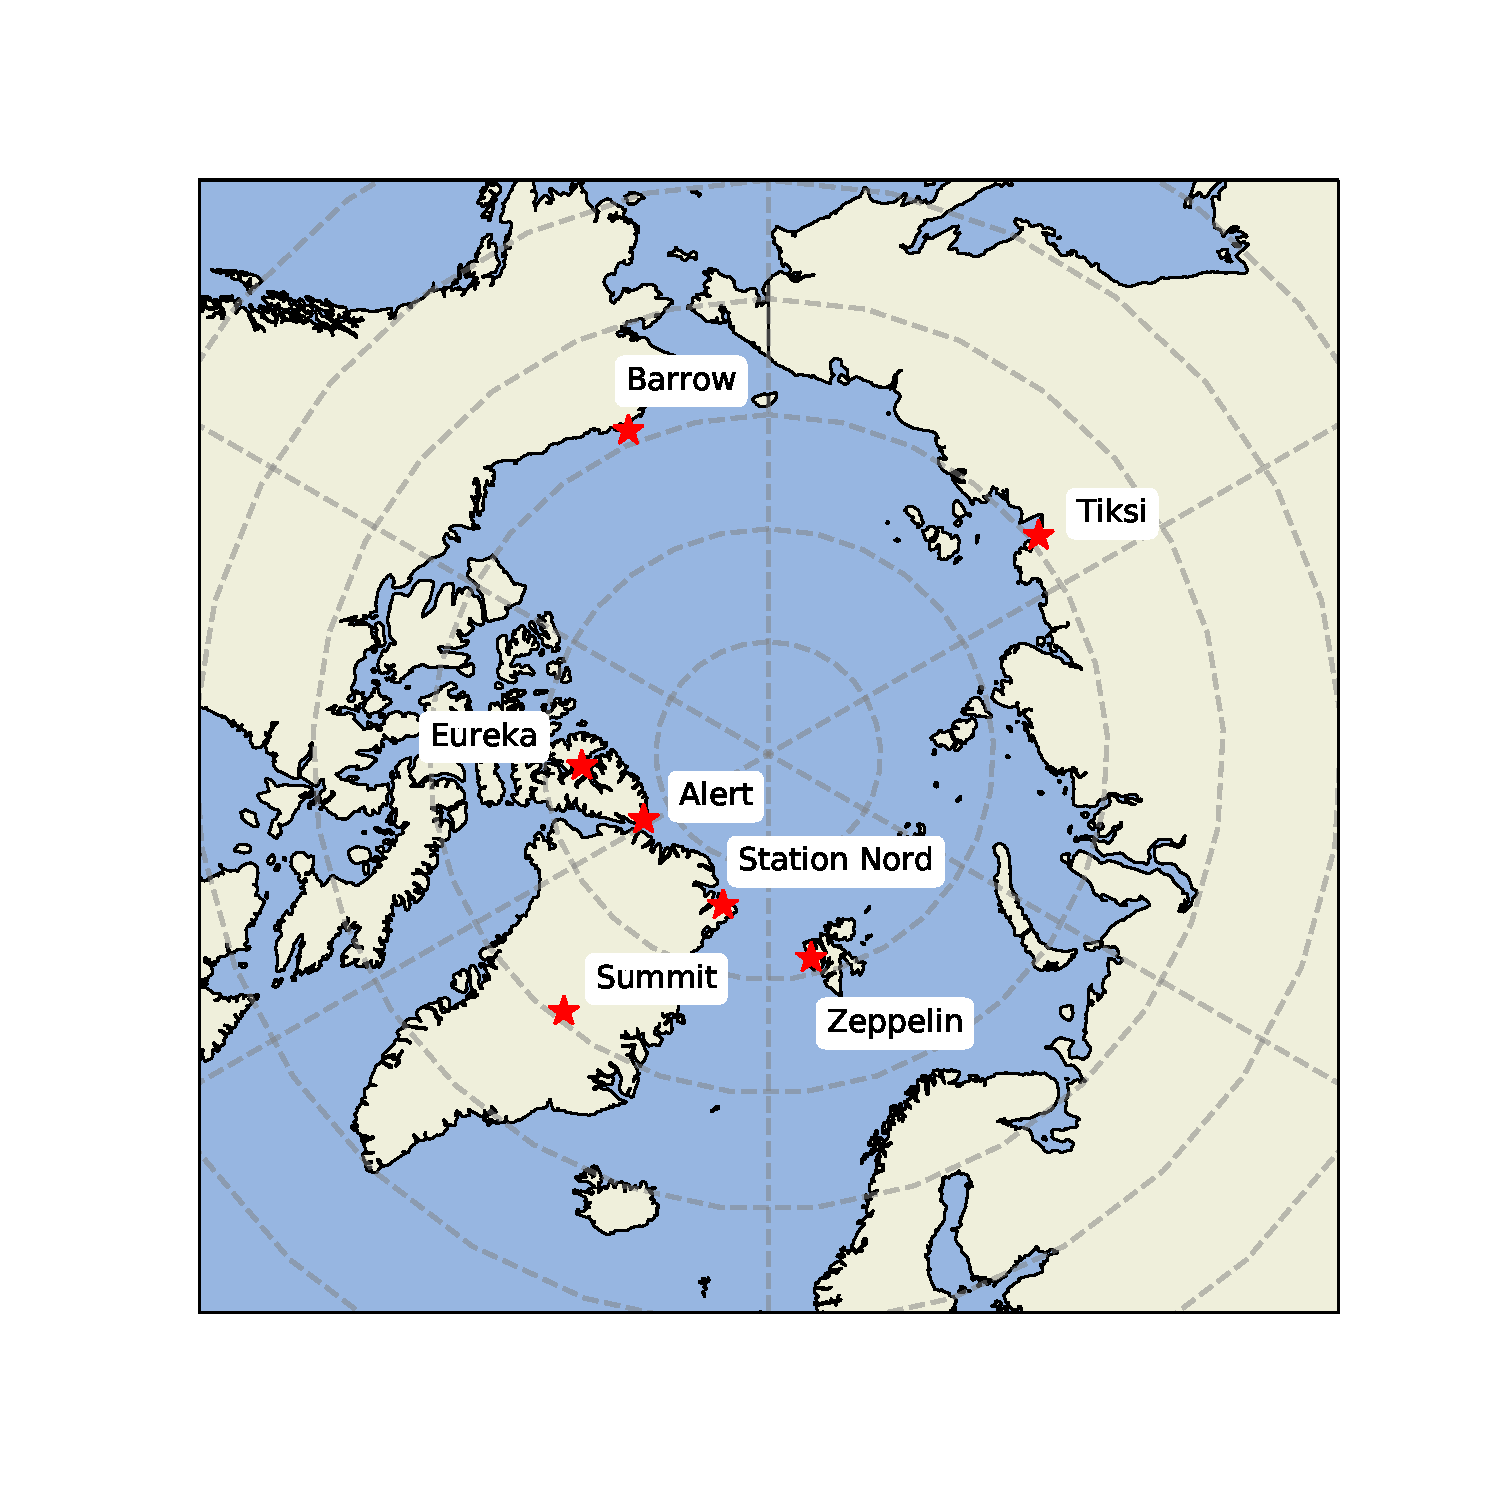
\includegraphics[width = .8\linewidth]{Chapter1_Intro/images/StationMap.pdf}
    \caption{Map of the stations used in comparison. Coordinates are listed in Table \ref{tab:stns}}
    \label{fig:stns}
\end{figure}
\begin{table}[h]
\centering
\resizebox{\columnwidth}{!}{%
\begin{tabular}{|llll|}
\hline
\textbf{Station}                 & \textbf{Location}       & \textbf{Altitude} & \textbf{Reference}     \\ \hline
Alert, Canada                    & 82$^o$50'N, 62$^o$34'W  & 210.0 m           & \cite{EBAS}, \cite{ESRL} \\
Barrow, Alaska, U.S.             & 71$^o$19'N, 156$^o$37'W & 11.0              & \cite{ESRL}            \\
Eureka, Canada                   & 80$^o$03'N, 86$^o$24'W  & 610.0 m           & \cite{EBAS}            \\
Station Nord, Greenland, Denmark & 81$^o$36'N, 16$^o$40'W  & 20.0 m            & \cite{EBAS}            \\
Summit, Greenland, Denmark       & 72$^o$34'N, 38$^o$28'W  & 3238.0 m          & \cite{EBAS}, \cite{ESRL} \\
Tiksi, Siberia, Russia           & 71$^o$58'N, 128$^o$92'E & 8.0 m             & \cite{EBAS}, \cite{ESRL} \\
Zeppelin, Svalbard, Norway       & 78$^o$54'N, 11$^o$53'E  & 474.0 m           & \cite{EBAS}            \\ \hline
\end{tabular}
}
\caption{Information about stations used in the comparison of model results and measured ozone}
\label{tab:stns}
\end{table}

\subsection{Code Availability}\label{sec:code_availability}

The Oslo CTM3 v1.1 is available on GitHub at \url{https://github.com/NordicESMhub/OsloCTM3}. The developing branches I have used are called:

%\begin{itemize}
%    \item \texttt{marikoll\_originalCTM3\_NoStrat}: present day, original CTM3, no stratosphere 
%    \item \texttt{marikoll\_originalCTM3\_noStrat\_pi}: pre-industrial, original CTM3, no stratosphere
%    \item \texttt{marikoll\_bromine\_explosion\_susanne}: present day, halogen chemistry, no stratosphere
%    \item \texttt{marikoll\_bromine\_explosion\_PI}: pre-industrial, halogen chemistry, no stratosphere
%\end{itemize}

\begin{mydef}\label{def:origCTM3_PD}
    \texttt{marikoll\_originalCTM3\_NoStrat}: present day, original CTM3, no stratosphere
\end{mydef}

\begin{mydef}\label{def:origCTM3_PI} 
    \texttt{marikoll\_originalCTM3\_noStrat\_pi}: pre-industrial, original CTM3, no stratosphere
\end{mydef}
    
\begin{mydef}\label{def:BE_PD}
    \texttt{marikoll\_bromine\_explosion\_susanne}: present day, halogen chemistry, no stratosphere (called susanne as the code was adapted from \cite{Susanne})
\end{mydef}
    
\begin{mydef}\label{def:BE_PI}
    \texttt{marikoll\_bromine\_explosion\_PI}: pre-industrial, halogen chemistry, no stratosphere
\end{mydef}
%\cleardoublepage

\setcounter{chapter}{1} 
\chapter{Theoretical Background: the Chemistry of the Arctic Troposphere} \label{ch:theoretical_back}

This chapter provides the background theory for the thesis. It concerns the chemistry of ozone, the impact on the radiative balance, and the heterogeneous reactions causing the depletion of ozone in the troposphere. Further, some of the sources of halogens as well as the mechanisms behind the halogen explosions are investigated. 

\begin{figure}
    \centering
    \includegraphics[width = 0.6\linewidth]{Chapter2_Theory/images/sea_ice.JPG}
    \caption{Sea ice in St. Jonsfjorden, Svalbard on 22 April at 23:00 UTC, 2018 (photograph: Private)}
    \label{fig:sea_ice}
\end{figure}


\section{Atmospheric radiation}\label{sec:atm_rad}

The Earth's energy balance is the balance between the incoming shortwave radiation from the Sun and the \acrfull{olr} that the Earth emits to space. The average temperature on Earth is fairly constant. Thus, radiant energy from the sun that is absorbed by the earth-atmosphere system must be re-emitted in order for the equilibrium energy state to be maintained. The emitted energy from the Earth is referred to as thermal \acrfull{ir} (\cite{Liou_AtmRad}, \cite{SeinfeldSpyros}). 

\medskip

Any imbalance occurring in the the Earth-atmosphere system due to external agents is quantified as the \acrfull{rf} (\cite{IPCCchapter8}, \cite{Bowman2013}). RF is usually expressed in watts per square meter over a particular period of time, such as pre-industrial to present day (\cite{IPCCchapter8}). The estimated RF change due to tropospheric $\chem{O_3}$ since pre-industrial times is estimated to be 0.40 (0.20 to 0.60) Wm$^{-2}$ (\cite{IPCCchapter8}). 


\medskip

Photodissociation of a molecule can occur when the energy of the photon exceeds the binding energy between the molecule's components (\cite{SeinfeldSpyros}). The photodissociation of ozone: $\chem{O_3} + hv \rightarrow \chem{O_2} + \chem{O}$, can yield various electronic states of the products \chem{O} and $\chem{O_2}$ depending on the wavelength of the incident radiation, with the singlet-D oxygen atom, $\chem{O}(^1\chem{D})$ being the most important electronically excited species of the atmosphere as it's reaction with water vapor is a source of \chem{OH} radicals, enhancing the oxidation capacity of the atmosphere (\cite{SeinfeldSpyros}).


\medskip

The absorption spectra of ozone is varying according to the strength of the chemical bands in the molecule. The strongest band (Hartley band - $\chem{O(^3P)}$ formation) absorbs highly energetic \acrfull{uv} radiation from the sun in the upper stratosphere and mesosphere in the wavelength range 242-310 nm. The UV Absorption spectrum of $\chem{O_2}$ is strongly connected to the formation of ozone, and absorbs in the range of 100-242 nm in the thermosphere, mesosphere and stratosphere. At about 50 km altitude, the maximum ozone absorption occurs in the Hartley band. In the lower stratosphere and troposphere, ozone absorbs solar flux in the range 310-400 nm (Huggins bands - $\chem{O(^3P)}$ formation). The weakest band (Chappuis bands) absorbs in the visible- and near IR region in the troposphere. The absorption range is 400-850 nm (\cite{Liou_AtmRad}). 



\medskip 

In the thermal infrared, ozone absorbs in two main bands, which are in the 9.6 and 14.27 $\mu$m regions. The latter band is overlapped by the $\chem{CO_2}$ 15 $\mu$m band. The atmospheric window is the wavelength range in which the atmosphere is relatively transparent. Thus, most IR absorption occurs outside the wavelength region 8-12 $\mu$m (\cite{AtmModFund}), which makes the 9.6 band the most important absorption band for ozone (\cite{Liou_AtmRad}, \cite{Myhre1997}). Due to it's absorption in the IR region, ozone is a gas that contributes to the greenhouse effect, i.e. it contributes to the trapping of thermal IR, and thus heating of the atmosphere (\cite{Liou_AtmRad}).



\section{Ozone and its precursors}

Ozone is a colorless gas that impacts the life on our planet in different ways, depending on the location of it's occurrence. If situated in the stratosphere (the ozone layer) it absorbs harmful UV radiation from the Sun in the range of 100-315 nm, and is thus essentially functioning as a shield for the planet (\cite{SeinfeldSpyros}). However, if located in the lower troposphere, ozone affects human health and vegetation. Concentrations above 0.1 \acrfull{ppm} interferes with the growth of plants, and has unhealthy impacts on humans (\cite{AtmModFund}). Typical concentrations in the free troposphere range from 20 to 40 \acrfull{ppb} near sea level and from 30 to 70 ppb at higher altitudes. In moderately to severely polluted urban areas, concentrations may range from 0.01 ppm to 0.35 ppm (\cite{AtmModFund}).  

\medskip

Stratospheric ozone has a natural origin, resulting from the photolytical decomposition of $\chem{O_2}$ followed by the oxygen atom reacting with another $\chem{O_2}$ molecule, thus producing two $\chem{O_3}$ molecules. The ozone molecules themselves may continue to react with other anthropogenic and/or naturally occurring stratospheric molecules. Generally, the concentration of $\chem{O_3}$ in the stratosphere is in steady-state due to the balance of it's production and destruction, and at the peak of the ozone layer, the $\chem{O_3}$ mixing ratio is about 12 ppm (\cite{SeinfeldSpyros}).  

\medskip

In the troposphere, ozone is a secondary pollutant resulting from two major classes of precursors; volatile organic compounds (VOCs) and oxides of nitrogen ($\chem{NO_x} = \chem{NO} + \chem{NO_2}$). In urban areas, $\chem{NO_x}$ mixing ratios range from 5 to 20 ppb. In rural areas, concentrations are about 1 ppb, and in remote areas, concentrations range from 10 to 100 ppt. In remote areas, ozone formation is sustained by $\chem{CH_4}$ and \chem{CO} through reactions with \chem{OH} (\cite{Cadle1970}, \cite{Levy1971}, \cite{SeinfeldSpyros}). The production of ozone is thus usually limited by the access of $\chem{NO_x}$ and $\chem{HO_x} (\chem{HO} + \chem{HO_2})$ (\cite{Levy1971}). The main removal pathways in the troposphere are through photolysis and through reaction with $\chem{HO_2}$ (\cite{SeinfeldSpyros}).

\medskip

One of the features of the stable Arctic boundary layer is the Arctic front. The front acts as a transport barrier that isolates the Arctic lower troposphere towards lower latitudes (\cite{BARRIE1986643}). In order to transport polluted air to the Arctic lower troposphere on a timescale of a few weeks, the source region of the pollution must be cold enough as well as located north of the Arctic front, which may extend down to about 40 $^o$N in January (\cite{BARRIE1986643}, \cite{AMAP2015}). 


\medskip

Both in the troposphere and the stratosphere, the $\chem{O_3}$ photolysis occurs, which produces both ground-state \chem{O} and excited singlet $\chem{O(^1D)}$ oxygen atoms (\cite{SeinfeldSpyros}): 

\begin{reaction}
    \chem{O_3} + hv \rightarrow \chem{O_2} + \chem{O}
    \label{rqn:groundstate_O2}
\end{reaction}

\begin{reaction}
    \chem{O_3} + hv \rightarrow \chem{O_2} + \chem{O(^1D)}
    \label{rqn:excited_O2}
\end{reaction}

The ground-state oxygen atom rapidly reacts with an oxygen molecule to re-form ozone, thus forming a null-cycle:

\begin{reaction}
    \chem{O} + \chem{O_2} + \chem{M} \rightarrow \chem{O_3} + \chem{M}
    \label{rqn:ozone}
\end{reaction}

Reaction \ref{rqn:ozone} is the most significant source of ozone in the atmosphere (\cite{SeinfeldSpyros}). The excited oxygen atom, however must react with another atmospheric species to rid itself from excess energy. Most often, it collides with $\chem{N_2}$ or $\chem{O_2}$, which removes the excess energy, quenching it back to it's ground state (\cite{Levy1971}). Every now and then, however, the excited oxygen atom may react with $\chem{H_2O}$ to form \chem{OH} radicals (\cite{SeinfeldSpyros}): 

\begin{reaction}
    \chem{O(^1D)} + \chem{H_2O} \rightarrow 2\chem{OH}
    \label{rqn:OH}
\end{reaction}

This is the only gas-phase reaction in the troposphere that is able to break the \chem{H-O} bond in $\chem{H_2O}$ (\cite{SeinfeldSpyros}). Tropospheric ozone is thus increasing the oxidizing capacity of the troposphere as it is acting as a precursor for \chem{OH}. The hydroxyl radicals interplay in a chain of reaction that results in the removal of atmospheric \chem{CO} and $\chem{CH_4}$ (\cite{Levy1971}). 

\medskip

When \chem{NO} and $\chem{NO_2}$ is present in sunlight, ozone may be produced photochemically (i.e. the initiating step is the absorption of a photon (\cite{Cadle1970})) in by the photolysis of $\chem{NO_2}$ (Reaction \ref{rqn:no2hv} below) followed by Reaction \ref{rqn:ozone} (\cite{Hesstvedt1978}): 


\begin{reaction}
    \chem{NO_2} + hv \rightarrow \chem{O} + \chem{NO}
    \label{rqn:no2hv}
\end{reaction}

The \chem{NO}-molecule quickly reacts with ozone to regenerate $\chem{NO_2}$:


\begin{reaction}
    \chem{O_3} + \chem{NO} \rightarrow \chem{O_2} + \chem{NO_2}
    \label{rqn:o3no}
\end{reaction}




\section{Halogen chemistry}


The halogens are a group in the periodic table consisting of fluorine, chlorine, bromine and iodine, as well as astatine, which is incredibly rare and therefore not considered to be of importance in the case of ozone depletion caused by reactive halogens. Natural occurrence of halogens and halogen-containing compounds can be found in sea water (as well as other sources, which will not be considered here). The halogens that pay partake in ozone depletion occur in the following abundance (more abundant to less abundant); chloride, bromide and iodide (\cite{Simpson2015}). 

\medskip

Even though bromide is less abundant than chloride, it is most prone to participate in the depletion of ozone. The reason for this is that chlorine has a similar bond strength with hydrogen as it has with hydrocarbons (such as methane), and is therefore prone to react with hydrocarbons rather than act to deplete ozone: 

\begin{reaction}
    \chem{Cl} + \chem{CH_4} \rightarrow \chem{HCl} + \chem{CH_3}
    \label{R:cl_ch4}
\end{reaction}

In a field study at Alert conducted by \cite{Foster2001}, they found $\chem{Br_2}$ and \chem{BrCl} molecules in relation with \acrshort{ode}. $\chem{Cl_2}$ on the other hand, was below the detection limit throughout the measuring period, indicating that the chlorine compound that is active in the ODEs is \chem{BrCl}- 

\medskip

Bromine, on the other hand, is less reactive towards hydrocarbons and readily depletes ozone in a catalytic manner.  Fluorine creates strong bonds with hydrogen, and is thus not reactive towards ozone. Aqueous iodine is less abundant than bromine and chlorine in the ocean due to it's role as a nutrient for biological systems (\cite{FinlaysonPitts2010}, \cite{Simpson2015}). 

\medskip

Thus, the focus in this thesis will be bromide, and to some extent chlorine reactive species. The reactive halogens have short lifetimes on the order of seconds to minutes and are typically only present during the day as they are activated by photolysis:



\begin{reaction}
    \chem{BrCl} + hv \rightarrow \chem{Br} + \chem{Cl}
    \label{R:19}
\end{reaction}

\begin{reaction}
    \chem{Br_2} + hv \rightarrow 2\chem{Br}
\end{reaction}

Throughout this and the following section, halogen species which partake in ozone depletion will be denoted as "\chem{X}". Reactive halogens denotes radical species such as atomic halogen species, \chem{X}, and their higher oxides, \chem{XO}. 

\begin{reaction}
    \chem{X_2} + hv \rightarrow 2\chem{X} \label{R:1}
\end{reaction}

The absorption spectra of dihalogens lies in the actinic (visible to near-UV) part of the spectra. Thus, photolysis may occur at longer wavelengths than that of ozone photochemistry, which requires UV photons near 300 nm (Photolysis of ozone is highly dependent on ozone column at higher altitudes, see Section \ref{sec:atm_rad}) (\cite{Simpson2015}).

\medskip

Halogen reservoir species are nonradicals that sequester reactive halogens. These include species such as $\chem{X_2}$, $\chem{HOX}$, $\chem{XONO_2}$ and $\chem{HX}$. The halogen reservoir species are less reactive, and hence the lifetime of theirs are longer than the reactive species (\cite{Simpson2015}). Moreover, \cite{Foster2001} found that $\chem{Br_2}$ and \chem{BrCl} were produced in high amounts at the time when polar sunrise occurred. This may point to a build-up of photolabile halogen species during the polar night. A similar theory was suggested by Simpson et.al. (\cite{Simpson2018}) who found that peak \chem{BrO} concentrations were found in airmasses that had been exposed to minimal photolysis of $\chem{Br_2}$ (Utquiavik (Barrow), Alaska). More information about halogen sources can be found in Section \ref{sec:halogen_sources}. 



\subsection{Bromine explosion}\label{sec:BE}

The discovery of ODEs in the troposphere due to anomalously high concentrations of reactive halogen species, bromine in particular, was made by Barrie and coworkers at Alert in Canada in 186-1987 (\cite{BARRIE1986643}). Ozone depletion was a well known phenomena at this point, but was unexplained until then (e.g. \cite{Oltmans1981}). 

\medskip

During polar spring, the amount of ozone in the polar boundary layer may decrease from tens of ppb to less than 1 ppb due to catalytic destruction by reactive halogen species (\cite{CAO}). the reaction scheme assuming bromine is the depleting agent is to a large extent summarized in Figure \ref{fig:het_react}. 

\medskip

\begin{figure}
    \centering
    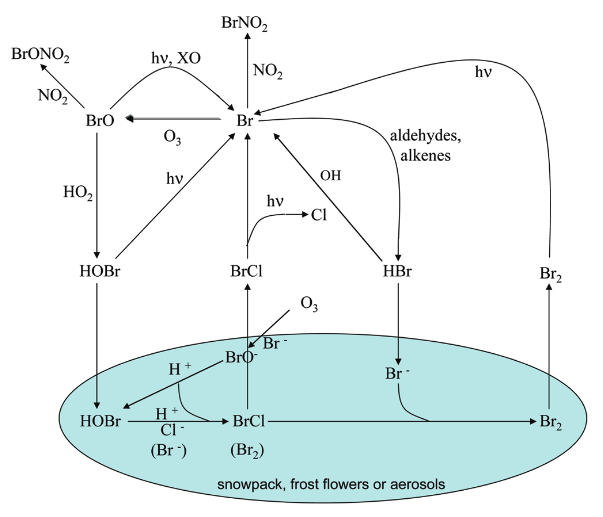
\includegraphics[width=0.7\linewidth]{Chapter2_Theory/images/ODE_Finlayson-Pitts.png}
    \caption{Typical heterogeneous reaction model. The blue shaded area illustrates the condensed phase. Image taken from \cite{FinlaysonPitts2010}}
    \label{fig:het_react}
\end{figure}


The production of halogen radicals and subsequent ozone depletion may proceed as follows (The set of reactions is taken from \cite{CAO} and \cite{Simpson2015}): 

\medskip

Reaction \ref{R:1} produces two halogen radicals, which are highly reactive. Ozone is then destroyed by: 

\begin{reaction}
    \chem{X} + \chem{O_3} \rightarrow \chem{XO} + \chem{O_2}
    \label{R:2}
\end{reaction}

The halogen oxides may proceed to deplete ozone. They partition quickly between the the following reactions and either reactivate by Reaction \ref{R:1}, or becoming radical directly:


\begin{reaction}
    \chem{XO} + \chem{XO} \rightarrow \chem{X_2} + \chem{O_2} \label{R:3} 
\end{reaction}


\begin{reaction}
    \chem{XO} + \chem{XO} \rightarrow \chem{X} + \chem{X} + \chem{O_2} \label{R:4} 
\end{reaction}


\begin{reaction}
    \chem{XO} + \chem{XO} \rightarrow \chem{OXO} + \chem{X} \label{R:5} 
\end{reaction}

The \chem{XO}-self reaction in Reactions \ref{R:3} to \ref{R:5} are often considered the rate limiting step for $\chem{O_3}$ destruction (\cite{JPL}). The partitioning between \chem{XO} and \chem{X} is rapid (\cite{Schmidt} reported a $[\chem{XO}]/[\chem{X}]$ ratio globally close to 1). In addition to the partitioning in Reactions \ref{R:3} to \ref{R:5}, \chem{XO} may be oxidized or photolysed:  

\begin{reaction}
    \chem{OH} + \chem{XO} \rightarrow \chem{X} + \chem{HO_2}
    \label{R:15}
\end{reaction}

\begin{reaction}
    \chem{XO} + hv \rightarrow \chem{X} + \chem{O}
    \label{R:20}
\end{reaction}

The halogen oxides quickly photodissociate (on the order of seconds and minutes time scale) and Reactions \ref{R:2} and \ref{R:20} creates a null cycle that does not destroy or produce ozone. This has an effect on the partitioning of \chem{X} and \chem{XO} species. The oxides dominate the radical form, which extends the lifetime of the $\chem{XO_x} = \chem{X} + \chem{XO}$-family as the oxides are generally less reactive than the atomic form (\cite{Simpson2015}). 

\medskip

Termination reactions that renders the \chem{XO}-radical into the reservoir species \chem{HBr}, \chem{HOBr} and $\chem{BrONO_2}$ may proceed as follows: 

\begin{reaction}
    \chem{XO} + \chem{HO_2} \rightarrow \chem{HOX} + \chem{O_2}
    \label{R:6} 
\end{reaction}

\begin{reaction}
    \chem{X} + \chem{HO_2} \rightarrow \chem{HX} + \chem{O_2}
    \label{R:17}
\end{reaction}


\begin{reaction}
    \chem{OH} + \chem{XO} \rightarrow \chem{HX} + \chem{O_2}
    \label{R:16}
\end{reaction}

\begin{reaction}
    \chem{BrO} + \chem{NO_2} + M \rightarrow \chem{BrONO_2} + M
    \label{R:9}
\end{reaction}

Depending on their relative bond strength, the reservoir species may be reactivated by: 


\begin{reaction}
    \chem{BrO} + \chem{NO} \rightarrow \chem{NO_2} + \chem{Br}
    \label{R:14}
\end{reaction}



\begin{reaction}
    \chem{BrONO_2} + \chem{H_2O} \xrightarrow{aerosol} \chem{HOBr} + \chem{HNO_3}
    \label{R:13}
\end{reaction}

\begin{reaction}
    \chem{HOBr} + hv \rightarrow \chem{Br} + \chem{OH}
    \label{R:18}
\end{reaction}


The bromine explosion events involves reaction \ref{R:1}, \ref{R:2} and \ref{R:6}, with $\chem{X} = \chem{Br}$, in an autocatalytic manner by the means of heterogeneous reactions: 

\begin{reaction}
    \chem{HOBr} + \chem{X^-_{aq}} + \chem{H^+_{aq}} \xrightarrow{snow/ice} \chem{BrX} + \chem{H_2O} \label{R:7} 
\end{reaction}
\begin{reaction}
    \chem{HOBr} + \chem{HX_{aq}} \xrightarrow{aerosol} \chem{BrX} + \chem{H_2O} \label{R:8}
\end{reaction}



In which the multiphase Reactions \ref{R:7} and \ref{R:8} outlines the release of bromine radicals from the condensed phase on snow/ice surfaces or aerosol surfaces, respectively. In this case, \chem{X} may denote \chem{Br} or \chem{Cl}, normally. The full multiphase reaction is dependent on temperature, sunlight and an acidic reaction surface (\cite{Toyota}). The bromine explosion can be summed up as follows: 

\begin{align*}
    \chem{HOBr} + \chem{X^-_{aq}} + \chem{H^+_{aq}} &\xrightarrow{snow/ice} \chem{BrX} + \chem{H_2O} \\
    \chem{Br_2} + hv &\rightarrow 2\chem{Br} \\
    \chem{Br} + \chem{O_3} &\rightarrow \chem{BrO} + \chem{O_2} \\
    \chem{BrO} + \chem{HO_2} &\rightarrow \chem{HOBr} + \chem{O_2} \\
    \text{NET:} \quad \chem{X^-_{aq}} + \chem{H^+_{aq}} + \chem{HO_2} + \chem{O_3}  &\rightarrow \chem{Br} + \chem{H_2O} + 2\chem{O_2} 
\end{align*}

\medskip

The reactive surface maybe supplied by different media, and this is an object of many research articles (e.g.  \cite{Simpson2018}, \cite{Rankin}). Whichever is more significant, there is most likely a cooperation of the reactive surfaces that accelerates the bromine explosion events. The reactive surfaces are (generally): 

\begin{itemize}
    \item Newly formed sea ice: Has a higher salinity and a higher bromine content than old sea ice and sea water \cite{Rankin}
    \item Snow surfaces, with low pH
    \item Aerosol surfaces, with low pH
\end{itemize}

\subsubsection{Chlorine reservoir species}

In the stratosphere, $\chem{NO_2}$ and $\chem{CH_4}$ are responsible for shifting reactive chlorine species into reservoir species (\cite{SeinfeldSpyros}). Methane acts via Reaction \ref{R:cl_ch4} to form $\chem{CH_3}$. Reservoir compounds may form by the reaction of \chem{XO} and $\chem{NO_2}$: 

\begin{reaction}
    \chem{ClO} + \chem{NO_2} + M \rightarrow \chem{ClONO_2} + M
    \label{R:clono2}
\end{reaction}

\subsection{Halogen sources}\label{sec:halogen_sources}

Sources of reactive halogens in the troposphere include photochemical degradation of organobromines ($\chem{CHBr_3}$, $\chem{CH_2Br_2}$, $\chem{CH_3Br}$), release of bromine from \acrfull{ssa} and transport from the stratosphere (\cite{Schmidt}). 

\medskip

Model studies has shown that the release of reactive halogen species from SSA is particularly relevant in polar regions (\cite{Schmidt}). While SSA is a known and certain source of reactive bromine species in the Arctic, the surface on which sea salt is transformed into gas-phase reactive halogens is somewhat unclear (\cite{Simpson2005}). SSA is formed though the breaking of waves at the ocean surface (\cite{Simpson2015}). 

\medskip

Formation of reactive halogen species though frost flowers has been suggested as a potential source. Frost flowers are ice crystals that forms on new sea ice when air that is supersaturated with water vapor condenses at the surface of the ice (\cite{GRANFORS2013124}, \cite{Kaleschke}). However, the sporadic nature and short lifetime of frost flowers points to other sources that may be more prominent as ODEs occur frequently during the polar spring. Snowpack measurements over coastal- and central Arctic \acrfull{fyi} and remote \acrfull{myi} performed by \cite{Peterson2019} revealed mostly snowpacks enriched in bromide species as a potential source of reactive bromine. This suggests that both MYI and FYI plays a role in the activation of halogens that subsequently may deplete ozone. The halides are incorporated in the snowpack by transported snow containing SSA (\cite{Toyota}, \cite{Peterson2019}). Trace bromine gases, such as \chem{HBr}, \chem{HOBr} and $\chem{BrONO_2}$, may be produced in the snowpack or deposited through mulitphase-reactions (\cite{Simpson2005}). 


\medskip


In the marine boundary layer, chlorine is the most abundant halide and is released from SSA by as $\chem{HCL}$ by acid displacement and photochemically as reactive halogens or their precursors. There is a difference between the marine boundary layer in polar regions and outside polar regions with respect to observed contents of $\chem{BrO}$ and $\chem{BrCl}$. Observations of these species rarely exceed detection limits and in the case of $\chem{BrCl}$, it is hardly observed at all (\cite{Simpson2015}). 

\medskip

The ocean also provides a large source of bromine- and iodide containing halocarbons that, when emitted into the troposphere, comprise very short-lived species (VSLS) that influence ozone destruction both in the troposphere and stratosphere (\cite{ziska}, \cite{Simpson2015}). The most abundant short-lived halocarbon (containing bromine) in the atmosphere and ocean are bromoform ($\chem{CHBr_3}$) and dibromomethane ($\chem{CH_2Br_2}$). Bromoform and dibromomethane is produced by marine organisms such as macroalgae and phytoplankton (\cite{Quack2003}).


\medskip

The oxidation of $\chem{CHBr_3}$ and $\chem{CH_2Br_2}$ as well as the photolysis of $\chem{CHBr_3}$ is applied as a source for tropospheric $\chem{Br_y}$ in this set-up following \cite{Parella}:


\begin{reaction}
    \chem{CHBr_3} + \chem{OH} \rightarrow 3\chem{Br} + \chem{Products}
    \label{R:10}
\end{reaction} 
\begin{reaction}
    \chem{CH_2Br_2} + \chem{OH} \rightarrow 2\chem{Br} + \chem{Products}
    \label{R:11}
\end{reaction}
\begin{reaction}
    \chem{CHBr_3} + hv \rightarrow 3\chem{Br} + \chem{Products}
    \label{R:12}
\end{reaction}

\medskip

Reactive bromine species and their precursors may also be transported, either within the Arctic boundary layer (\cite{Luo2018}, \cite{Schmidt}), or from the stratosphere. 


\subsection{Influence of nitrogen}


Generally, tropospheric ozone is a result of two main precursors, $\chem{NO_x} = \chem{NO} + \chem{NO_2}$

In polluted regions, there is an important balance between regions with too much $\chem{NO_x}$, which generally acts as a precursor of ozone, and areas where the $\chem{NO_x}$ concentration is low enough to sustain the production of ozone depleting reactive halogens. The high concentrations of $\chem{HNO_3}$ and $\chem{H_2SO_4}$ can in theory provide the reactive surfaces for acidity dependent autocatalytic release of reactive halogens, but the efficiency of this mechanism is degraded in the case of $\chem{NO_x}$ and hydrocarbon concentrations (\cite{Simpson2015}). High concentrations of $\chem{NO_x}$ suppresses the formation of $\chem{HO_x}$, which is in turn a key component of the halogen explosion sequence. Hydrocarbons serve as sinks for reactive halogens due to their willingness to react with these rather than with ozone, and thus terminates the halogen explosion sequence (\cite{Simpson2015}). Incidents in which halogens do get activated in polluted regions, production of nitryl halides, $\chem{XNO_2}$, is considered to be a major activation process. Observations have shown that this is mostly relevant for chlorine as the reactivity and/or solubility of $\chem{BrNO_2}$ and $\chem{INO_2}$ are likely much greater than for $\chem{ClNO_2}$ \cite{Simpson2015}. 

\medskip





\cite{SeinfeldSpyros} SKRIV OM HIGH NOX/LOW NOX ENVIRONMENTS

In the troposphere, ozone is a secondary pollutant produced in areas with high anthropogenic emissions of $\chem{NO_x}$. 
\cleardoublepage

\setcounter{chapter}{2} 
\chapter{Theoretical Background: Processes Implemented in the CTM3}\label{Chap:CTM3theory_ocean_hetReact}

Some of the processes that are implemented in the Oslo CTM3 requires some further explanation. Here, I will cover the theory behind the implementation of emissions of organic halogen species and the heterogeneous reaction surfaces.

\section{Oceanic Emissions of Halocarbons}\label{sec:oceanic_emissions}


The ocean is a natural source of gaseous halocarbons, and is therefore used here as a source needed for the bromine explosion to occur. Methyl halides ($\chem{CH_3X}$) and polyhagenated species ($\chem{CHBr_3}$, $\chem{CH_2Br_2}$) are released from the ocean, but methyl halides (particularly $\chem{CH_3Br}$) may also be emitted by biomass burning (\cite{SeinfeldSpyros}). 

\medskip

Bromoform ($\chem{CHBr_3}$) and dibromomethane ($\chem{CH_2Br_2}$) are used as the oceanic sources of bromine in this implementation. The anthropogenic signal of methyl halides are not taken into consideration in this thesis. Nor are the difference in lifetime ($\chem{CH_3Br} \sim$ 1 month, $\chem{CH_2Br_2} \sim$ 4 months) as well as seasonal variations. 


\medskip

Bromoform, $\chem{CH_3Br}$, is added as a source from the ocean based on the emission scenario suggested by \cite{Liang2010} (scenario A, Figure \ref{fig:Liang2010}). This scenario was chosen as it has latitudinal-dependent emission field covering the whole globe. The global emissions estimated by \cite{Liang2010}, scenario A, were 425 Ggyr$^{-1}$ of $\chem{CHBr_3}$ and 57 Ggyr$^{-1}$ of $\chem{CH_2Br_2}$, respectively.

\medskip

The thought behind the implementation (the variable \texttt{POLL\_CHBr3}) is that it contains the emissions from both $\chem{CHBr_3}$ and $\chem{CH_2Br_2}$. The reason for this is that there was already an organic halogen existing in the CTM3, methyl bromide ($\chem{CH_3Br}$), which would only be used by the model when the stratosphere was activated (which was not the case in my runs). Thus, this was used for the mapping of the concentration of $\chem{CHBr_3}$ and $\chem{CH_2Br_2}$ instead. To simplify this source further, $\chem{CH_2Br_2}$ was added to the emission scheme in Figure \ref{fig:Liang2010} by a scaling factor based on the global emissions. 

\medskip

The scaling factor was calculated by finding the yield of bromine from both $\chem{CHBr_3}$ and $\chem{CH_2Br_2}$ based on reactions \ref{R:10} and \ref{R:11}, and expressing this in terms of $\chem{CHBr_3}$. 

\begin{align*}
    \chem{X} & = 57 Gg \chem{CH_2Br_2}yr^{-1} \\
    \chem{Y} & = 425 Gg \chem{CHBr_3}yr^{-1} 
\end{align*}

The bromine yield, \chem{Z}, from Reactions \ref{R:10} and \ref{R:11} is then: 

\begin{align*}
    \chem{Z} & = \Big(3\cdot\Big(\frac{X}{M_{\chem{CH_2Br_2}}}\Big) + 2\cdot\Big(\frac{Y}{M_\chem{CHBr_3}}\Big)\Big)\cdot M_{\chem{Br}} \\
    & = \Big(3\cdot\Big(\frac{425 Gg \chem{CHBr_3}yr^{-1}}{252.73 g mol^{-1}}\Big) + 2\cdot\Big(\frac{57 Gg \chem{CH_2Br_2}yr^{-1}}{173.83 g mol^{-1}}\Big)\Big)\cdot79.90 g mol^{-1} \\
    & = 455 Gg\chem{Br}yr^{-1}
\end{align*}

The emission of $\chem{CHBr_3}$, had this been the only source of bromine, is expressed by $Y'$, which is: 

\begin{align*}
    \chem{Y'} & = \frac{1}{3}\cdot\frac{252.73 g mol^{-1}}{79.90 g mol^{-1}}\cdot455.49Gg\chem{Br}yr^{-1} \\
    & = 479.73 Gg \chem{CHBr_3}yr^{-1}
\end{align*}

This is used in the scaling factor, $f$:

\begin{equation*}
    f = \frac{\chem{Y'}}{Y} \approx 1.13
\end{equation*}


Emissions are then found according to their latitudinal band, and whether the grid box is located over ocean or the coast (for more information about the actual implementation, see Section \ref{sec:tropchem_oslo}). If the location is above 50 $^o$ North over ocean, for example, the emission is taken to be $0.05\times10^{-13}$ kgm$^{-2}$s$^{-1}\times k$. (The conversion to molecules cm$^{-3}$s$^{-1}$ can be seen in Section \ref{sec:tropchem_oslo}). 


\subsection{Emission inventory}

The emission inventory of $\chem{CHBr_3}$ and $\chem{CH_2Br_2}$ by \cite{Liang2010} was compared against observations and other emission inventories by \cite{Hossaini2013}. The results can be seen in Figures \ref{fig:Hosaini_fig5} and \ref{fig:Hosaini_fig6} in the Appendix. They show a reasonable agreement between the observations and mixing ratios suggested by \cite{Liang2010} for the stations \acrfull{alt}, \acrfull{brw} and Summit (SUM), which are of most relevance in this setting. The inventory, however is rather crude and simple as it does not take into account seasonality, extrapolar results of agreement with observations. 


\begin{figure}
    \centering
    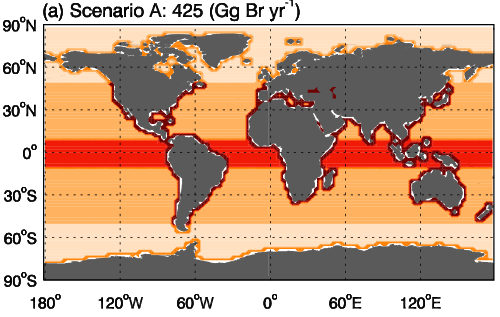
\includegraphics[width = 0.5\textwidth]{Chapter3_Theory_ocean_hetReact/images/liang_etal_2010.png}
    \caption{Global emission distribution of $\chem{CHBr_3}$. Scenario A is applied for the \chem{CHBr_3} with emissions taken as the half point of the colorbar. Image taken from \cite{Liang2010}}
    \label{fig:Liang2010}
\end{figure}


\section{Chemical Kinetics}\label{sec:chem_kinetics}

This section contains a description of the rate expressions for bimolecular and 3-body reactions. The reaction rate constants for the bimolecular, and 3-body reactions implemented in the troposphere can be seen in Table \ref{tab:2b_and_3b_reactions}

\begin{table}[ht]
\centering
\resizebox{14cm}{!}{%
\begin{tabular}{|c|ccc|c|c|c|l|}
\hline
\multicolumn{8}{|c|}{\textbf{Reactions dependent on temperature (Bimolecular reactions)}}                                                                                                                                                                                                                                                                                                         \\ \hline
\textbf{Reaction}                                                    & \multicolumn{1}{c|}{\textbf{A-factor}}    & \multicolumn{2}{c|}{\textbf{E/R}}                                            & \textbf{k (273.15 K) (*)}                          & \multicolumn{3}{l|}{\textbf{Reaction ref.}}                                                                            \\ \hline
$\chem{Cl} + \chem{CH_4} \rightarrow \chem{HCl} + \chem{CH_3} $      & \multicolumn{1}{c|}{$7.3\cdot10^{-12}$}   & \multicolumn{2}{c|}{$1280$}                                                  & $6.7\cdot10^{-14}$                             & \multicolumn{3}{c|}{\ref{R:cl_ch4}}                                                                                    \\
$\chem{O_3} + \chem{Br} \rightarrow \chem{BrO} + \chem{O_2}$         & \multicolumn{1}{c|}{$1.7\cdot10^{-11}$}   & \multicolumn{2}{c|}{$800$}                                                   & $9.1\cdot10^{-13}$                             & \multicolumn{3}{c|}{\ref{R:2}}                                                                                         \\
$\chem{O_3} + \chem{Cl} \rightarrow \chem{ClO} + \chem{O_2}$         & \multicolumn{1}{c|}{$2.3\cdot10^{-11}$}   & \multicolumn{2}{c|}{$200$}                                                   & $1.1\cdot10^{-11}$                             & \multicolumn{3}{c|}{\ref{R:2}}                                                                                         \\
$\chem{BrO} + \chem{BrO} \rightarrow 2\chem{Br} + \chem{O_2}$        & \multicolumn{1}{c|}{$2.4\cdot10^{-12}$}   & \multicolumn{2}{c|}{$-40$}                                                   & $2.8\cdot10^{-12}$                             & \multicolumn{3}{c|}{\ref{R:4}}                                                                                         \\
$\chem{OH} + \chem{ClO} \rightarrow \chem{Cl} + \chem{HO_2}$         & \multicolumn{1}{c|}{$7.4\cdot10^{-12}$}   & \multicolumn{2}{c|}{$-270$}                                                  & $2.0\cdot10^{-11}$                             & \multicolumn{3}{c|}{\ref{R:15}}                                                                                        \\
$\chem{BrO} + \chem{HO_2} \rightarrow \chem{HOBr} + \chem{O_2}$      & \multicolumn{1}{c|}{$4.5\cdot10^{-12}$}   & \multicolumn{2}{c|}{$-460$}                                                  & $2.4\cdot10^{-11}$                             & \multicolumn{3}{c|}{\ref{R:6}}                                                                                         \\
$\chem{Br} + \chem{HO_2} \rightarrow \chem{HBr} + \chem{O_2}$        & \multicolumn{1}{c|}{$4.8\cdot10^{-12}$}   & \multicolumn{2}{c|}{$310$}                                                   & $1.5\cdot10^{-12}$                             & \multicolumn{3}{c|}{\ref{R:17}}                                                                                        \\
$\chem{OH} + \chem{ClO} \rightarrow \chem{HCl} + \chem{O_2}$         & \multicolumn{1}{c|}{$6.0\cdot10^{-13}$}   & \multicolumn{2}{c|}{$-230$}                                                  & $1.4\cdot10^{-12}$                             & \multicolumn{3}{c|}{\ref{R:16}}                                                                                        \\
$\chem{BrO} + \chem{NO} \rightarrow \chem{NO_2} + \chem{Br}$         & \multicolumn{1}{c|}{$8.8\cdot10^{-12}$}   & \multicolumn{2}{c|}{$-260$}                                                  & $2.3\cdot10^{-11}$                             & \multicolumn{3}{c|}{\ref{R:14}}                                                                                        \\
$\chem{CHBr_3} + \chem{OH} \rightarrow 3\chem{Br} + \chem{Products}$ & \multicolumn{1}{c|}{$1.35\cdot10^{-12}$}  & \multicolumn{2}{c|}{$600$}                                                   & $1.5\cdot10^{-13}$                             & \multicolumn{3}{c|}{\ref{R:10}}                                                                                        \\ \hline
\multicolumn{8}{|c|}{\textbf{Reactions dependent on pressure and temperature (3-body reactions)}}                                                                                                                                                                                                                                                                         \\ \hline
\multirow{2}{*}{\textbf{Reaction}}                                   & \multicolumn{3}{c}{\textbf{Low-Pressure Limit}}                                                                          & \multicolumn{3}{c|}{\textbf{High-Pressure Limit}}                                                                             & \multirow{2}{*}{\textbf{Reaction ref.}} \\ \cline{2-7}
                                                                     & \multicolumn{1}{c|}{\textbf{k$_0^{300}$}} & \multicolumn{1}{l|}{\textbf{n}} & \multicolumn{1}{l|}{\textbf{k$_0^{300}$ (273.15 K) (**)}} & \multicolumn{1}{l|}{\textbf{k$_\infty^{300}$}} & \multicolumn{1}{l|}{\textbf{m}} & \multicolumn{1}{l|}{\textbf{k$_\infty^{300}$ (273.15 K) (***)}} &                                         \\ \hline
$\chem{BrO} + \chem{NO_2} + M \rightarrow \chem{BrONO_2} + M$        & \multicolumn{1}{c|}{$5.2\cdot10^{-31}$}   & \multicolumn{1}{c|}{$3.2$}      & $7.0\cdot10^{-31}$                         & $6.9\cdot10^{-12}$                             & $2.9$                           & $9.0\cdot10^{-12}$                         & \multicolumn{1}{c|}{\ref{R:9}}          \\
$\chem{NO_2} + \chem{ClO} + M \rightarrow \chem{ClONO_2} + M $       & \multicolumn{1}{c|}{$1.8\cdot10^{-31}$}   & \multicolumn{1}{c|}{$3.4$}      & $2.5\cdot10^{-31}$                         & $1.5\cdot10^{-11}$                             & $1.9$                           & $1.8\cdot10^{-11}$                         & \multicolumn{1}{c|}{\ref{R:clono2}}     \\ \hline
\end{tabular}
}
\caption{Rate coefficients for some of the bimolecular and 3-body reactions implemented in the troposphere. Values are taken from \cite{JPL}. Rate coefficients are calculated at 273.15 K by: 
\\ 
(*) k is calculated by Equation \ref{eq:2b_rate_coeff} 
\\ 
(**) k$_0^{300}$ is calculated by Equation \ref{eq:3b_low_pressure} 
\\ 
(***) k$_\infty^{300}$ is calculated by Equation \ref{eq:3b_high_pressure}} 
\label{tab:2b_and_3b_reactions}
\end{table}

\subsection{Bimolecular Reactions}\label{sec:bimolecular_reactions}

Bimolecular reactions are reactions in which two chemical species react and produce a different set of species (\cite{Jacob1999}). The reaction can be written as: 

\begin{equation*}
    A + B \rightarrow C + D
\end{equation*}

%A direct bimolecular reaction is a reaction in which \chem{A} and \chem{B} goes on to produce \chem{C} and \chem{D} without an intermediate formation of an \chem{AB}-bond, but rather has a transition state $(\chem{AB})^\neq$ that lies between the reactants and products (\cite{JPL}). 

%\medskip

%The correlation between the expected structure of $(\chem{AB})^\neq$ and the A-factor (Arrhenius factor) of the the reaction rate constant


The reaction rate, $k$, is the time rate of change of a concentration of the reactant in the reaction (\cite{AtmModFund}). It is given by: 

\begin{equation*}
    -\frac{d}{dt}[A] = -\frac{d}{dt}[B] = \frac{d}{dt}[C] = \frac{d}{dt}[D] = k[A][B]
\end{equation*}

in which the bracketed species $[]$ denotes the number densities (in this case the number of molecules per $cm^3$) and $k$ is the second-order rate coefficient for the reaction in $cm^3\text{molecule}^{-1}s^{-1}$. The product $[A][B]$ is proportional to the frequency of collisions. A bimolecular reaction could also be a self-reaction, in which $B = A$ and the reaction rate would be:

\begin{equation*}
    -\frac{d}{dt}[A] = -\frac{d}{dt}[A] = \frac{d}{dt}[C] = \frac{d}{dt}[D] = k[A]^2
\end{equation*}

The rate coefficients are given in Table \ref{tab:2b_and_3b_reactions} in Arrhenius form (for more information, see \cite{JPL}):

\begin{equation}
    k(T) = A\cdot\exp{\Big(-\frac{E/R}{T}\Big)}
    \label{eq:2b_rate_coeff}
\end{equation}

In which $A$ is the Arrhenius-factor, $E/R$ is the temperature dependence (activation temperature) and $T$ is the temperature. 

\subsection{3-Body Reactions}\label{sec:3body_reactions}

Three-body reactions are reactions in which two chemical species, \chem{A} and \chem{B}, react to produce one single product species, \chem{AB}, helped by a third body, $M$ (\cite{Jacob1999}). The reaction can be written as: 

\begin{equation*}
    \chem{A} + \chem{B} + M \rightarrow \chem{AB} + M
\end{equation*}


The third body, $M$, is an inert molecule (generally $\chem{N_2}$ or $\chem{O_2}$ in the atmosphere) that removes excess energy from the excited species $\chem{AB*}$ leaving the product species \chem{AB} in it's unexcited state (\cite{Jacob1999}).


\medskip

%The rate coefficient for a 3-body reaction is defined as the formation rate of AB by the reaction of $M$ with the excited complex $[\chem{AB}^*]$: 

%\begin{equation*}
%    \frac{d[\chem{AB}]}{dt} = k_3[\chem{AB}^*][M]
%\end{equation*}

%This rate is assumed to be in steady state at all times as $[\chem{AB}^*]$ is very short lived, which leads to the following expression: 

%\begin{equation*}
%    k_1[\chem{A}][\chem{B}] = k_2[\chem{AB}^*] + %k_3[\chem{AB}^*][M]
%\end{equation*}

The rate coefficients for 3-body reactions can be pressure dependent, and therefore have a low-pressure and high-pressure limit. The low pressure limiting rate constants are given in Table \ref{tab:2b_and_3b_reactions} on the form: 

\begin{equation}
    k_0(T) = k_0^{300}\Big(\frac{T}{300}\Big)^{-n}    
    \label{eq:3b_low_pressure}
\end{equation}

In which $k_0^{300}$ is an estimate of the low-pressure limiting rate constant at 300 K. $n$ is the estimated temperature dependence at the low-pressure limit (for more information, see \cite{JPL}). The low pressure rate constants is of third order and has units $cm^6\text{molecule}^{-1}s^{-1}$ (\cite{AtmModFund}).

\medskip

Similarly, there exists a high-pressure limit:

\begin{equation}
    k_\infty(T) = k_\infty^{300}\Big(\frac{T}{300}\Big)^{-m}
    \label{eq:3b_high_pressure}
\end{equation}

In which $k_\infty^{300}$ is an estimate of the high-pressure limiting rate constant at 300 K. $m$ is the estimated temperature dependence at the high-pressure limit (for more information, see \cite{JPL}). The high-pressure rate constant is of second order and has units $cm^3\text{molecule}^{-1}s^{-1}$ (\cite{AtmModFund}).


\section{Photochemical reactions}

For photochemical reactions, the rate expression is (\cite{AtmModFund}):

\begin{equation*}
    A + hv \rightarrow B + C
\end{equation*}

and the rate expression is: 

\begin{equation*}
    \frac{d[A]}{dt} = -J[A]
\end{equation*}

In which $J$ is a first-order photolysis rate coefficient of species $A$ (units: $s^-1$). 


Kan legge inn tabell med D-ratene her 

\section{Heterogeneous chemistry}\label{sec:het_chem}

Skriv kort om heterogene reaksjoner og legg inn hvilke som er lagt inn i CTM3 i tabell

\subsection{Heterogeneous Reactions on Aerosol Surfaces (Reactions \ref{R:8} and \ref{R:13})}\label{sec:aerosol_react}

The implementation of the heterogeneous aerosol Reactions \ref{R:13} and \ref{R:8} is based on the method described by \cite{CAO}. An overview of the constants used can be found in Table \ref{tab:constants}.

\medskip

The explanation for Reaction \ref{R:8} will be for $\chem{X} = \chem{Br}$, but the same applies to $\chem{X} = \chem{Cl}$. Reaction \ref{R:13} is differently treated ($\gamma$ is parameterized), and is explained further in Section \ref{sec:het_aerosol_react_CTM3}. The production rate of $\chem{Br_2}$ molecules for Reaction \ref{R:8} is (\cite{schwartz1986}): 

\begin{equation*}
    \frac{d}{dt}[\chem{Br_2}] = -\frac{d}{dt}[\chem{HOBr}] = k[\chem{HOBr}]
\end{equation*}

which has the first-order reaction-rate constant which is dependent on the concentration of \chem{HBr}: 

\begin{equation}
    k = \big(\frac{a}{D_g} + \frac{4}{v_{therm}\gamma}\big)^{-1}\alpha_{eff}
    \label{eq:reaction_rate_const}
\end{equation}

$a$ is a typical aerosol radius (taken as $a = 0.45 \mu m$), $D_g$ is the molecular diffusivity in the gas-phase (taken as $D_g = 0.2  cm^2s^{-1}$), and the ratio $a/D_g$ represents the molecular diffusion limit (\cite{CAO}). 

\medskip

$v_{therm}$ in Equation \ref{eq:reaction_rate_const} is the mean molecular speed of \chem{HOBr} as the impinging gas on the aerosol surface. This is given as:

\begin{equation*}
    v_{them} = \sqrt{\frac{8RT}{\pi \chem{M_{HOBr}}}}
\end{equation*}

in which $R$ is the universal gas constant (in $Latm/Kmol$), $T$ is the absolute temperature in Kelvin,  and $\chem{M_{HOBr}}$ is the molas mass of \chem{HOBr}. $v_{therm}$ has units $cm/s$. 

\medskip

Finally, the two remaining parameters of Equation \ref{eq:reaction_rate_const} are $\gamma$ and $\alpha_{eff}$. $\gamma$ is the uptake coefficient or reaction efficiency of \chem{HOBr} on sea salt aerosols, i.e. the probability that the reaction will occur (\cite{SeinfeldSpyros}). $\alpha_{eff}$ is the surface-volume coefficient, i.e. the ratio of the total aerosol surface area, $A_{\text{aerosol}}$, and the total volume, $V$ and has the units $[cm^2cm^{-3}]$.
 
\medskip

The production rate of $\chem{Br_2}$ in Reaction \ref{R:8} is limited by the absorption of \chem{HOBr} and \chem{HBr} in the suspended aerosol particles (\cite{CAO}). The probability of the reaction, i.e. the uptake coefficient for \chem{HOBr}, $\gamma$,  can be expressed as (\cite{Hanson1994}) (Values are listed in Table \ref{tab:constants}): 

\begin{equation}
    \frac{1}{\gamma} = \frac{1}{\alpha}+ \frac{v_{therm}}{4H^*RT\sqrt{k_{liq}^ID_{liq}}f(q)}
    \label{eq:upt_coeff}
\end{equation}

in which $\alpha$ is the mass accommodation coefficient. This quantity describes the probability that a gas or vapour particle will stick upon collision with the surface of a particle, where $0\leq\alpha\leq1$ (\cite{SeinfeldSpyros}). Following \cite{CAO}, this will be taken as unity. As before, $R$ is the universal gas constant and $T$ is the temperature. $D_{liq}$ is the liquid phase diffusion coefficient which is a proportionality factor implying that a mass of the substance diffuses through a unit surface in a unit time at a concentration gradient of unity. $H^*$ is the effective Henry's law constant for \chem{HBr}. The Henry's law coefficient, $H$, is a proportionality factor between the amount of dissolved gas and it's partial pressure in the gas phase (\cite{Sander2015}, see also Section \ref{sec:wet_dep_henrys_law}). $k_{liq}^I$ is the first-order liquid reaction rate constant for \chem{HBr}, calculated by: 

\begin{equation}
    k_{liq}^I = k_{liq}^{II}[\chem{HBr}]_{liq}= k_{liq}^{II}H^*_\chem{HBr}P_\chem{HBr}
\end{equation}

In which $H^*_\chem{HBr}$ is the effective Henry's law constant for the species. $P_\chem{HBr}$ is it's partial pressure given by:

\begin{equation*}
    P_\chem{HBr} = \frac{\chem{M_{HBr}}RT}{Av}
\end{equation*}

which is where the dependence of the concentration of \chem{HBr} (in molecules$cm^{-3}$) appears, by $\chem{M_{HBr}}$. $R$ is the universal gas constant (converted from $LatmK^{-1}mol^{-1}$ to $10^3cm^3K^{-1}mol^{-1}$). $T$ is the temperature in Kelvin, and $Av$ is Avogadros number. 

\medskip

Lastly, $f(q)$ in Equation \ref{eq:upt_coeff} is determined by: 

\begin{equation}
    f(q) = \coth{q} -\frac{1}{q} = \frac{1}{\tanh{q}} -\frac{1}{q}
\end{equation}

where $q = a\sqrt{\frac{k_{liq}^I}{D_{liq}}}$, is a dimensionless quantity called the diffuso-reactive parameter. This is used to calculate the uptake rates (\cite{Hanson1994}). 


\subsection{Heterogeneous Reactions Over Snow and Ice Surfaces (Reactions \ref{R:7})}\label{sec:snow_ice_react}


The implementation of the heterogeneous reactions over snow/ice surfaces also follows the method by \cite{CAO}. 

\medskip

The rate of change in concentration for Reactions \ref{R:7} can be given as: 

\begin{equation*}
    -\frac{d}{dt}[\chem{HOBr}] = k[\chem{HOBr}]
\end{equation*}

in which the deposition-rate constant, $k$, is: 

\begin{equation*}
    k = \frac{v_d}{L_{mix}}\beta
\end{equation*}

Thus, the deposition-rate constant depends on the deposition velocity, $v_d$, at the snow/ice surface, the height of the boundary layer, $L_{mix}$ and the reactive surface ratio coefficient, $\beta$. 

\medskip

The deposition velocity, $v_d = (r_a + r_b + r_c)^{-1}$, is dependent on three resistances which are: 

\begin{itemize}
    \item The aerodynamic resistance, $r_a$. This is the resistance of the turbulent transport to bring the gas from the atmosphere to the surface, approximated as: $1/(u\kappa^2)(\ln(z/z_0))^2$, where $u = 8 ms^{-1}$ is the wind speed, $\kappa = 0.4$ is the Von Karman constant, $z$ is the surface layer height, approximated as the lower $10\%$ of the boundary layer, i.e. $z = 0.1L_{mix}$, and $z_0$ is the surface roughness length which is approximated as $10^{-5} m$ for ice surfaces. $r_a$ is therefor dependent on local properties. 
    \item The quasi-laminar layer resistance, $r_b$, is the ability of molecular diffusion to transfer gas across a liquid-laminar layer above the surface. It is thus given as $r_b = z_0/D_g$
    \item The resistance due to the reaction loss, $r_c$ is given as $r_c = 4/v_{therm}\gamma$. The uptake coefficient is taken as $\gamma = 0.06$ including the assumption that the source of $\chem{H^+}$ and halogen ions are limitless at the snow/ice surface. 
\end{itemize}

$L_{mix}$ denotes the typical stable boundary layer height which may, in Polar regions, range from near-zero up to approximately 1000 m depending on. Consequently, the deposition velocities vary.

\medskip

$\beta$ is the ratio of the total reactive surface (induced by the structure of snow/ice surfaces) to a flat area. Thus, for a completely flat surface, $\beta$ equals 1. 

\begin{table}[ht]
\centering
\resizebox{\columnwidth}{!}{%
\begin{tabular}{|llll|}
\hline
\textbf{Variable} & \textbf{Quantity}    & \textbf{Unit}       & \textbf{Description}                                       \\ \hline
\multicolumn{4}{|c|}{\textbf{\chem{HOBr}}}                                                                 \\ \hline
$\alpha$          & $1.0$                & Dimensionless       & Mass accommodation coefficient                             \\
$\alpha_{eff}$    & $1.0 \times 10^{-6}$ & $cm^{-1}$           & Surface-volume coefficient                                 \\
$a$               & $0.45$               & $\mu m$             & Typical aerosol radius                                     \\
$\beta$           &                      & Dimensionless       & Ratio of the total reactive surface area to a flat surface \\
$D_{liq}$         & $5.0\times10^{-6}$   & $cm^2s^{-1}$        & Liquid phase diffusion coefficient                         \\
$D_g$             & $0.2$                & $cm^2s^{-1}$        & Molecular diffusivity                                      \\
$H^*$             & $1.7 \times10^4$     & $molL^{-1}atm^{-1}$ & Effective Henry's law constant                             \\
$M_{\chem{HOBr}}$ & $96.91\times10^{-3}$ & $kg mol^{-1}$       & Molar mass of \chem{HOBr}                 \\ \hline
\multicolumn{4}{|c|}{\textbf{\chem{HBr}}}                                                                  \\ \hline
$H^*$             & $3.0\times10^{8}$    & $molL^{-1}atm^{-1}$ & Effective Henry's law constant                             \\
$k_{liq}^{II}$    & $5.0\times10^{4}$    & $L mol^{-1}s^{-1}$  & Second order liquid rate reaction constant                 \\ \hline
\multicolumn{4}{|c|}{\textbf{\chem{HCl}}}                                                                  \\ \hline
$H^*$             & $3.0\times10^{6}$    & $molL^{-1}atm^{-1}$ & Effective Henry's law constant                             \\
$k_{liq}^{II}$    & $1.0\times10^{5}$    & $L mol^{-1}s^{-1}$  & Second order liquid rate reaction constant                 \\ \hline
\multicolumn{4}{|c|}{\textbf{$\chem{BrONO_2}$}}                                                                             \\ \hline
$\gamma$          & $0.06$               & Dimensionless       & Effective uptake coefficient                               \\ \hline
\end{tabular}
}
\caption{Overview of constants taken from \cite{CAO}}
\label{tab:constants}
\end{table}



\section{Wet deposition and Henry's law}\label{sec:wet_dep_henrys_law}

Henry's law expresses the proportional relationship between the amount of gaseous and dissolved gas (\chem{A}) in equilibrium (\cite{SeinfeldSpyros}): 

\begin{equation*}
    \chem{A(g)} \rightleftharpoons \chem{A(aq)}
\end{equation*}

The proportionality factor is dependent on the partial pressure of \chem{A} in the gas phase and the dissolved \chem{A} such that: 

\begin{equation}
    [\chem{A(aq)}] = H_Ap_A
    \label{eq:Henryslaw}
\end{equation}

In which $H_A$ is the Henry's law coefficient and $p_A$ is the partial pressure of \chem{A(g)}. 

\medskip

In this context, and widely used by atmospheric chemists, the Henry solubility, $H^{cp}$ is applied (\cite{Sander2015}). Rearranging Equation \ref{eq:Henryslaw} gives: 

\begin{equation}
    H^{cp} \equiv \frac{C_A}{p_A}
    \label{eq:HenrySol}
\end{equation}

The temperature dependence of the Henry's law coefficient, which is an equilibrium constant, can be described by the van't Hoff equation (\cite{Sander2015} and references therein): 

\begin{equation*}
    \frac{d\ln(H)}{d(1/T)} = \frac{-\Delta_{sol}H}{R}
    \label{eq:vantHoff}
\end{equation*}

In which $\Delta_{sol}H$ is the change in enthalpy of dissolution ($H$ in this case does not refer to the Henry's law constant). $R$ is the universal gas constant. 


At equilibrium, the number of moles per liter of a gas that is dissolved in a droplet is given by Henry's law


The Henry's law constants can be seen in Section \ref{sec:scav_wet} in Table \ref{tab:Henrys_law}. 


\cleardoublepage

\setcounter{chapter}{3}
\chapter{Theoretical Background: Oslo CTM3}\label{chapt:OsloCTM3}

This chapter covers some of the functionality of the Oslo CTM3 that is of importance in the implementation of the halogen chemistry (Theory outlined in Chapter \ref{Chap:CTM3theory_ocean_hetReact} and the implementation process outlined in Chapter \ref{chap:CTM3_Setup}).

\section{The Oslo CTM3}

The Oslo CTM3 is a three-dimensional global chemical transport model. The model was developed at the Department of Geosciences at the University of Oslo and later at \acrfull{cicero} (\cite{SovdeManual}). It operates offline, driven by historical weather data from the \acrfull{ecmwf} \acrfull{openifs} model. The meteorological data is updated (offline) and stored every 3rd hour. The model spin-up time is 12h starting from an analysis at noon the day before (\cite{Sovde2012}). 

\medskip

The tropospheric chemistry in the CTM3 is a stand-alone module, while the stratosphere module requires the troposphere. Thus, there is a possibility of turning off the stratosphere to better isolate chemical processes occurring in the troposphere. In that case, the tropospheric species that are advected throughout the stratosphere are allowed to do so. The species are, however, not affected by any real chemistry but rather parameterized at the top of the troposphere based on their climatology. The species that are photolyzed in the stratosphere are instead set to decay at fixed rates, and species that have stratospheric origin (such as ozone and $\chem{NO_x}$) are set to model climatological values (climatological values produced by the CTM3 with stratosphere) (\cite{Sovde2012}).

\section{Transport of Species}\label{sec:CTM3_transport}

The transport time step in the Oslo CTM3 is usually 15 minutes for boundary layer mixing. For species with a much shorter lifetime than this, the concentration may change during the time step. The transport scheme in the CTM3 is therefore divided into transported- and non-transported species (\cite{SovdeManual}).

\medskip

The advection scheme in Oslo CTM3 is the UCI CTM transport core documented by \cite{Prather2008}. This is a 3D isotropic (same second order moment in all directions) advection scheme, where the zonal (U) and meridional (V) metereological fields are used to calculate the vertical field (W). An important feature of the advection scheme is the handling of the transport at the poles. Each polar-"pie" box is combined with its adjacent lower-latitude box (which conserves all moments) before [U] and [V] transport and restored to individual boxes afterwards, assuming unchanged polar pie air mass (\cite{Sovde2012}). 


\section{Photochemistry}\label{sec:CTM3_photochemistry}

The photodissocation rates (J-values) in $[s^{-1}]$ are calculated online using the fast-JX method, version 6.7c (\cite{FastJX}, \cite{SovdeManual}). The method calculates the photolysis rates (\texttt{J}-values) in the troposphere and the stratosphere from the surface up to 60 km altitude (\cite{Sovde2012}). 

\medskip

When only treating the troposphere, 20 photodissociation rates are calculated, whereas if the stratosphere is included, 51 rates are calculated. This is set automatically in \texttt{cmn\_size.F90} by the variable \texttt{JPPJ}. The reactions with photodissiciation rates associated to them are listed in \texttt{ratj\_oc.d}. 

\section{Solutions to Chemical Ordinary Differential Equations}

Modelling of the chemical processes in the atmosphere includes solving chemical ordinary differential equations. The method must have the ability to solve a system of equations with large variations in time constants, i.e. the lifetimes of species. A system such as this is known as a stiff system, and the difference in time constants leads to time-step limitations (\cite{AtmModFund}). In the Oslo CTM3, two approaches has been combined to solve these problems, which are the \acrfull{qssa} and the Family solution, which are in the following subsections. 

\subsection{QSSA-Integrator}\label{sec:QSSA}

The \acrshort{qssa} is a method that has the ability to solve a stiff system. It is mathematically quite simple, but has error bounds that are hard to estimate. However, in a global model like the CTM3, the use of a simple approach is necessary as it is computationally cheap and efficient (\cite{Hesstvedt1978}). 

\medskip

The QSSA method is described by \cite{Hesstvedt1978} as follows: 

\medskip

The time development of the concentration is given by the continuity equation:

\begin{equation}
    \frac{dC}{dt} = P - LC
    \label{eq:conteqn}
\end{equation}

In which $P$ and $LC$ are the photochemical production and loss terms, respectively. Assuming that $P$ and $L$ are constants over a time interval $\Delta t$, which is taken to be the step length in the numerical integration. Then, Equation \ref{eq:conteqn} has the analytical solution: 

\begin{equation}
    C_{t + \Delta t} = C_{E} + (C_{t} - C_{e})e^{-L\Delta t}
    \label{eq:analyt_soltn}
\end{equation}

In which $C_{e} = P/L$ is the photochemical equilibrium concentration. The characteristic time of variation (or photochemical lifetime) is defined as $\tau = 1/L$. According to $\tau$, the components in the system may be defined in the following three categories: 

\begin{enumerate}[label=(\roman*)]
    \item If $\tau < \Delta t/10$, the species' lifetime is considered short, and its concentration is calculated with the steady-state equation (assuming instant equilibrium with any other species):
    \begin{equation}
        C_{t + \Delta t} = \frac{P_{t + \Delta t}}{L_{t + \Delta t}}
        \label{eq:a}
    \end{equation}
    \item If $\Delta t \leq \tau \leq 100\Delta t$, the species' lifetime is considered moderate, and its concentration is calculated according to Equation \ref{eq:analyt_soltn}
    \item If $\tau \gg \Delta t$, the species' lifetime is considered long, and its concentration is calculated according to the simple Euler formula: 
    \begin{equation}
        C_{t + \Delta t} = C_t + (P_t - L_tC_t)\Delta t
        \label{eq:b}
    \end{equation}
\end{enumerate}

To obtain satisfactory accuracy with the QSSA method, it is important to use the correct category. Photochemical equilibrium can only be assumed when the lifetime of a given compound is much shorter than the time step (category (i)). If this is not the case, an exponential expression must be applied (category (ii)) (\cite{Hesstvedt1978}). The QSSA scheme is useful and accurate enough for applications in which calculations has to be repeated many times, but can only  be considered mass-conserving for long-lived species (\cite{AtmModFund}). 

\subsection{Family Solution to Ordinary Differential Equations}\label{sec:families}

Some groups of gases (families) has atoms transferring quickly among them, but are only slowly lost from the actual family. To obtain a numerically stable solution, it is more beneficial to integrate a family of components, as the family is more stable than the members of it. An example of a family is the odd oxygen family which includes: 

\begin{equation*}
    [\chem{O_T}] = [\chem{O}] + [\chem{O(^1D})] + [\chem{O_3}] + [\chem{NO_2}]
\end{equation*}

Oxygen atoms in the odd-oxygen family are cycled rapidly between the species atomic oxygen, excited atomic oxygen and ozone, but oxygen atoms are only slowly lost out of the family (\cite{AtmModFund}). The individual rates of production- and loss terms for the members in the family are calculated and summed up across the family. Then, the family concentration is integrated using the QSSA method. Finally, the individual members are scaled with the ratio of the individually integrated family and the sum of the individually integrated members of the family (\cite{SovdeManual}).

\medskip

The Oslo CTM3 uses the following family in the troposphere (\cite{SovdeManual}): 

\begin{equation*}
    \chem{NO_x} = \chem{NO} + \chem{NO_2} + \chem{NO_3} + 2\chem{N_2O_5} \chem{HO_2NO_2} + \chem{PAN}    
\end{equation*}

And the following families (among others) in the stratosphere:

\begin{align*}
    \chem{O_x} & = \chem{SO} = \chem{O_3} + \chem{O(^1D)} + \chem{O(^3P)} - \chem{NO} - \chem{CL} - \chem{Br} \\
    \chem{Br_y} & = \chem{Br} + \chem{BrO} + \chem{BrONO_2} + \chem{HOBr} + \chem{HBr} + 2\chem{Br_2} + \chem{BrCl} \\
    \chem{Cl_x} & = \chem{Cl} + \chem{ClO} + \chem{OHCl} + \chem{ClONO_2} + 2\chem{Cl_2} + \chem{OClO} + \chem{BrCl} + \chem{ClOO} + 2\chem{Cl_2O_2} \\
    \chem{Cl_y} & = \chem{Cl_x} + \chem{HCl}
\end{align*}

The advantages of using families are that is a fast method, and reasonably accurate for moderate- to low stiffness systems. However, the families needs to be carefully designed and validated, and the accuracy of the method decreases with increased stiffness (\cite{AtmModFund}).


\subsection{O3-NO Variable}\label{sec:O3-NO}

The strong coupling between the Reactions \ref{rqn:ozone}, \ref{rqn:no2hv} and Reaction \ref{rqn:o3no} cause numerical instability problems when choosing time steps that are too long (\cite{Hesstvedt1978}).

\begin{reaction}
    \chem{O_3} + \chem{NO} \rightarrow \chem{NO_2} + \chem{O_2}
    \label{rqn:o3no}
\end{reaction}

To avoid these instabilities, a new variable is defined: 

\begin{equation}
    x = [\chem{O_3}] - [\chem{NO}]
\end{equation}

The Euler expansion formula is then applied to calculate $x$. Next, the concentration of $\chem{O_3}$ or \chem{NO} may be calculated, depending on which is smaller, according to \textbf{i)}, \textbf{ii)} or \textbf{iii)} (\cite{Hesstvedt1978}). 

\setcounter{chapter}{4}
\chapter{Alteration made in the Oslo CTM3}\label{chap:CTM3_Setup}

This chapter describes the setup and altered modules of the Oslo CTM3. 

\section{Setup of The Model}

A degraded resolution was used for the runs in the CTM3. In the \texttt{Makefile} it is possible to degrade the horizontal resolution by combining several boxes into one. The setting used for running the model was \texttt{HWINDOW=HFOUR}, i.e. a combination of four native boxes and thus a $4.5^o \times 4.5^o$ resolution (Illustrated in Figure \ref{fig:res_map}). In the vertical, 60 layers were used. The setup of the \texttt{Makefile} is explained more in Appendix \ref{subsubsec:makefile}. 

\medskip

The stratosphere was turned off in all the branches in order to save CPU time and to avoid conflict with the organic bromide sources (see Section \ref{sec:oceanic_emissions}). How this was performed is explained in Appendix \ref{app:turning_off_the_stratosphere}. 

\begin{figure}[ht]
    \centering
    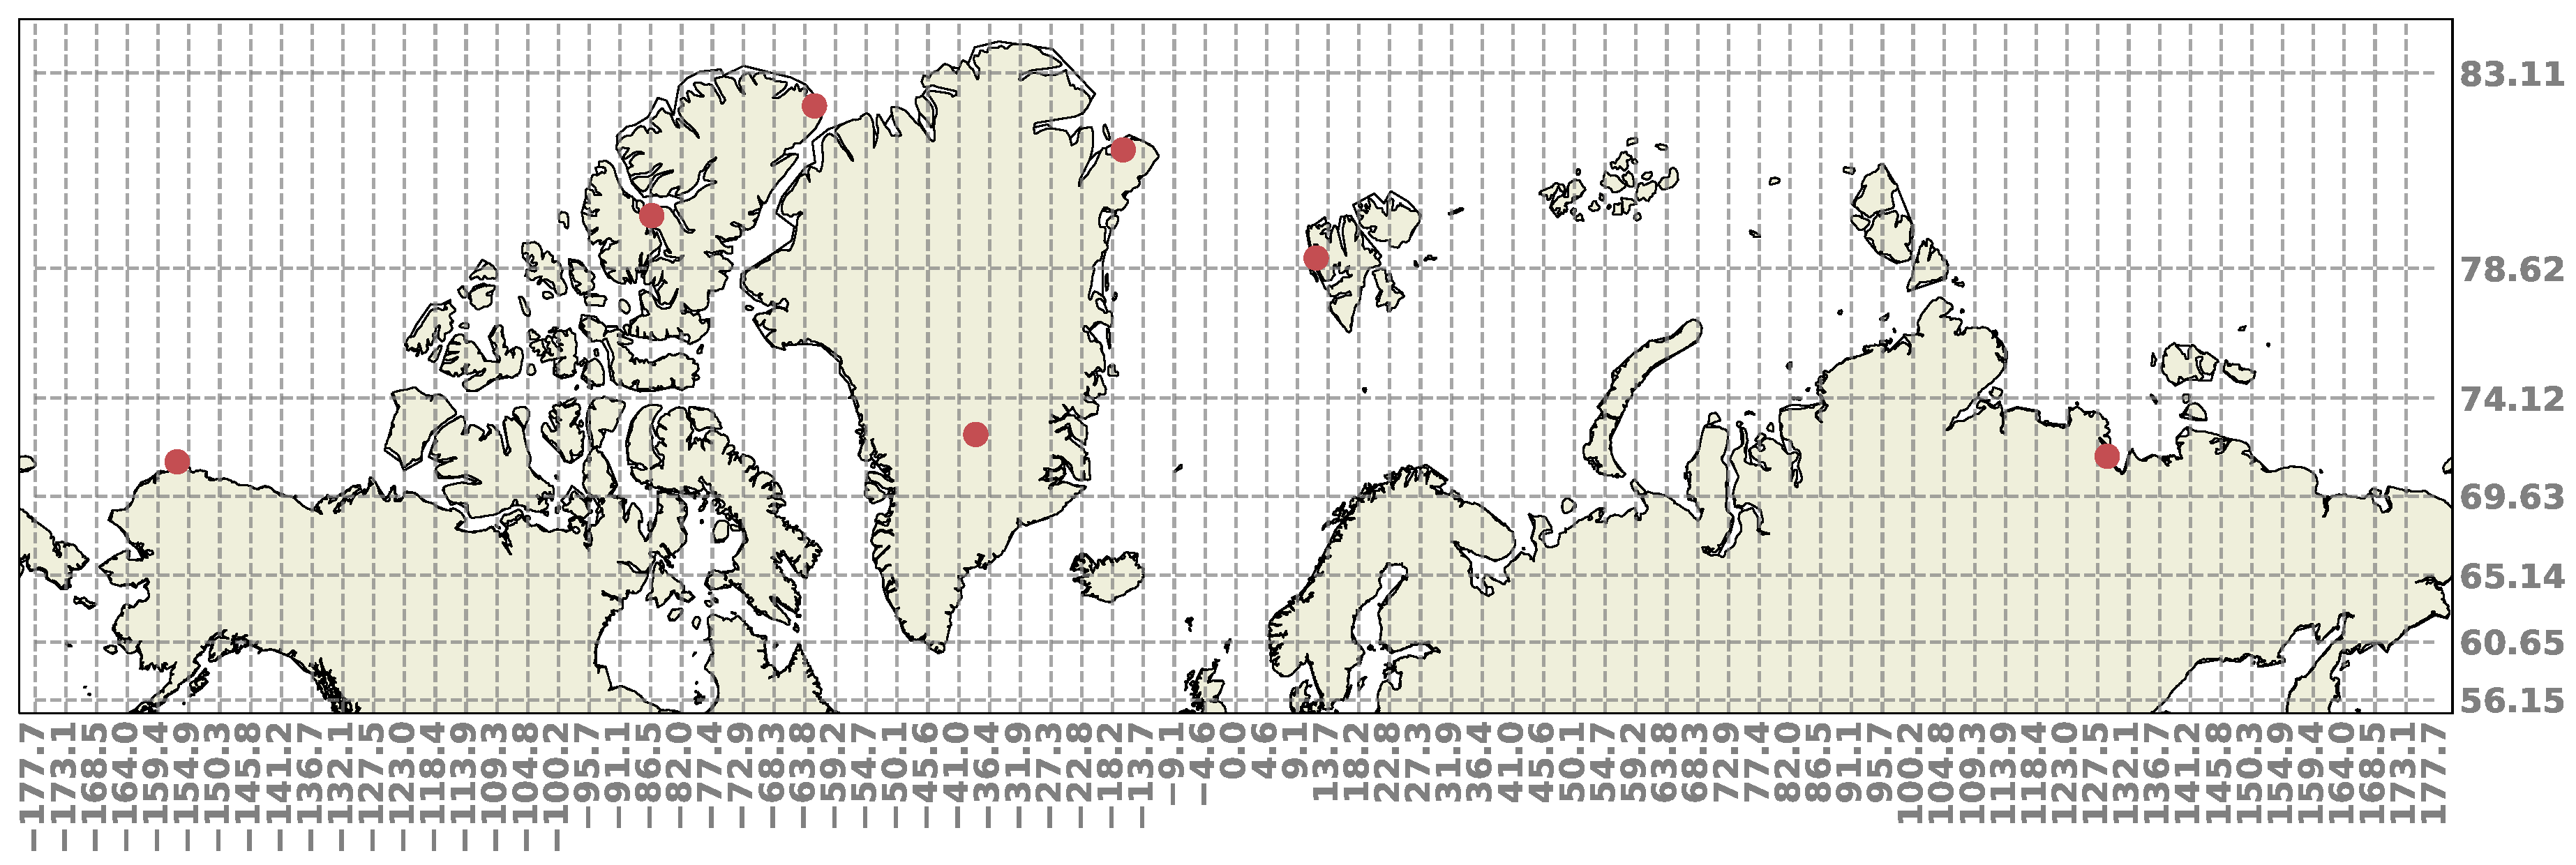
\includegraphics[width = \linewidth]{Chapter5_CTM3setup/images/resolution_map_Arctic.pdf}
    \caption{Illustration of the grid coverage in the Arctic at \texttt{HFOUR} $=$ 4.5$^o$x4.5$^o$ resolution. The red dots are the stations that were used for observational data}
    \label{fig:res_map}
\end{figure}


\medskip

To run the CTM3, a supercomputer is required. At the beginning of my master thesis the supercomputer Abel (\cite{abel}) was used. In January 2020, Abel was shut down and the Oslo CTM3 migrated to Saga (\cite{saga}). There are some differences between the two  and these differences as well as the setup of the model runs are explained in Appendix \ref{app:supercomputer}. 


\section{Wet deposition - \texttt{scavenging\_wet.inp}}\label{sec:scav_wet}

Wet scavenging rates for \chem{HCl}, \chem{HBr} and $\chem{ClONO_2}$ were added to the wet deposition input table \texttt{scavenging\_wet.inp}. The Henry's law constants are listed in Table \ref{tab:Henrys_law} and the wet deposition and Henry's law is explained in Section \ref{sec:wet_dep_henrys_law}. 

\begin{table}[ht]
\begin{tabular}{|lllll|}
\hline
\textbf{Component}          & \textbf{H$^{cp}$ [mol m$^{-3}$Pa]} & \textbf{$\frac{d \ln H^{cp}}{d(1/T)}$ [K]} & \textbf{Note} & \textbf{Reference}                \\ \hline
\chem{HCl} & $1.1\times10^{-2}$                     & $2300$                                         & (*)          & \cite{MARSH1985} \\
\chem{HBr} & $2.4\times10^{-1}$                     & $370$                                          & (**)         & \cite{dean1999}  \\
$\chem{ClONO_2}$            &  $2.1\times10^{5}$.   & $8700$                              & (***)       & \cite{Lelieveld1991TheRO}      \\ \hline
\end{tabular}
\caption{The Henry's law constants are taken from \cite{Sander2015} and references therein. 
\\
(*) Thermodynamical calculation  
\\ 
(**) Only the tabulated data between T = 273 K and T = 303 K from Dean (1992) were used to derive H and its temperature dependence. Above T = 303 K, the tabulated data could not be parameterized very well. The partial pressure of water vapor (needed to convert some Henry's law constants) was calculated using the formula given by Sander et al. (1995). The quantities A and $\alpha$ from Dean (1992) were assumed to be identical. 
\\ 
(***) Assumed to have the same Henry's law as $\chem{HNO_3}$ \cite{TerjePersonal}
\\
\textbf{Note: the units of the Henry's law constants were changed after this implementation (see the Results Section \ref{sec:res_step3}. It was changed to atm M$^{-1}$}}
\label{tab:Henrys_law}
\end{table}

 


\section{Implementation of halogen chemistry}

In essence, three modules were changed to implement the halogen chemistry. They were \texttt{pchemc\_ij.f90}, \texttt{tropchem\_oslo.f90} and \texttt{chem\_oslo\_rates.f90}. The base for the scripting is the work performed by \cite{Susanne}, which I have continued to alter.  The reactions that were implemented in the various modules can be seen in Table \ref{tab:3}.


%Some of the problems that occurred during this process, how these were tested and attemptedly solved, can be seen in Section \ref{chap:problem_solving}.
\begin{table}[ht]
\centering
\resizebox{12cm}{!}{%
\begin{tabular}{|l|l|l|}
\hline
\multicolumn{1}{|l|}{\textbf{Variable name CTM3}} & \multicolumn{1}{l|}{\textbf{Reaction}}                                                    & \textbf{Reaction no.}      \\ \hline
%\texttt{hobr\_dep}               & $\chem{HOBr} + \chem{HBr} \xrightarrow{aerosol} \chem{Br_2} + \chem{H_2O}$                & \ref{R:8} \\
\texttt{hobr\_dep}               & $\chem{HOBr} + \chem{H^+} + \chem{Br^-} \xrightarrow{snow/ice} \chem{Br_2} +\chem{H_2O} $ & \ref{R:7} \\
%\texttt{hobr\_dep}               & $\chem{HOBr} + \chem{HCl} \xrightarrow{aerosol} \chem{BrCl} + \chem{H_2O} $               & \ref{R:8} \\
\texttt{hobr\_dep}               & $\chem{HOBr} + \chem{H^+} + \chem{Cl^-} \xrightarrow{snow/ice} \chem{BrCl} +\chem{H_2O} $ & \ref{R:7} \\
\texttt{no2\_bro}                & $\chem{BrO} + \chem{NO_2} + M \rightarrow \chem{BrONO_2} + M$                             & \ref{R:9} \\
\texttt{oh\_chbr3}               & $\chem{CHBr_3} + \chem{OH} \rightarrow 3\chem{Br} + \chem{Products}$                      & \ref{R:10} \\
\texttt{oh\_chbr3}               & $\chem{CH_2Br_2} + \chem{OH} \rightarrow 2\chem{Br} + \chem{Products}$                    & \ref{R:11} \\
%\texttt{DCH\_3Br}                & $\chem{CHBr_3} + hv \rightarrow 3\chem{Br} + \chem{Products}$                             & \ref{R:12} \\ 
\texttt{brono2\_h2o}             & $\chem{BrONO_2} + \chem{H_2O} \xrightarrow{aerosol} \chem{HOBr} + \chem{HNO_3}$           & \ref{R:13}\\
\texttt{hobr\_hcl}               & $\chem{HOBr} + \chem{HCl} \xrightarrow{aerosol} \chem{BrCl} + \chem{H_2O}$                & \ref{R:8} \\
\texttt{hobr\_hbr}               & $\chem{HOBr} + \chem{HBr} \xrightarrow{aerosol} \chem{Br_2} + \chem{H_2O}$                & \ref{R:8} \\
\texttt{o3\_cl}                  & $\chem{O_3} + \chem{Cl} \rightarrow \chem{ClO} + \chem{O_2}$                              & \ref{R:2} \\
\texttt{no\_bro}                 & $\chem{BrO} + \chem{NO} \rightarrow \chem{NO_2} + \chem{Br}$                              & \ref{R:14} \\
\texttt{oh\_clo\_a}              & $\chem{OH} + \chem{ClO} \rightarrow \chem{Cl} + \chem{HO_2}$                              & \ref{R:15} \\
\texttt{oh\_clo\_b}              & $\chem{OH} + \chem{ClO} \rightarrow \chem{HCl} + \chem{O_2}$                              & \ref{R:16} \\
\texttt{br\_o3}                  & $\chem{O_3} + \chem{Br} \rightarrow \chem{BrO} + \chem{O_2}$                              & \ref{R:2} \\
\texttt{br\_ho2}                 & $\chem{Br} + \chem{HO_2} \rightarrow \chem{HBr} + \chem{O_2}$                             & \ref{R:17} \\
\texttt{bro\_ho2}                & $\chem{BrO} + \chem{HO_2} \rightarrow \chem{HOBr} + \chem{O_2}$                                    & \ref{R:6} \\
\texttt{bro\_bro}                & $\chem{BrO} + \chem{BrO} \rightarrow 2\chem{Br} + \chem{O_2}$                             & \ref{R:4} \\
\texttt{DHOBr}                   & $\chem{HOBr} + hv \rightarrow \chem{Br} + \chem{OH}$                                      & \ref{R:18} \\
\texttt{DCH3Br}                  & $\chem{CHBr_3} + hv \rightarrow 3\chem{Br} + \chem{Products}$                             & \ref{R:12} \\
\texttt{DBrCl}                   & $\chem{BrCl} + hv \rightarrow \chem{Br} + \chem{Cl}$                                      & \ref{R:19} \\
\texttt{DBrO}                    & $\chem{BrO} + hv \rightarrow \chem{Br} + \chem{O}$                                        & \ref{R:20} \\
\texttt{DBr2}                    & $\chem{Br_2} + hv \rightarrow 2\chem{Br} $                                                & \ref{R:1} \\
\texttt{cl\_ch4}                    & $\chem{Cl} + \chem{CH_4} \rightarrow \chem{HCl} + \chem{CH_3} $                                                & \ref{R:cl_ch4} \\
texttt{no2\_clo}                    & $\chem{NO_2} + \chem{ClO} + M \rightarrow \chem{ClONO_2} + M $                                                & \ref{R:clono2} \\
\hline
\end{tabular}
}
\caption{Reactions implemented in the troposphere}
\label{tab:3}
\end{table}


\subsection{Changes in \texttt{pchemc\_ij.f90}:}

\texttt{pchem\_ij} is a module that works as a column driver for the Oslo tropospheric chemistry. It has one subroutine, \texttt{OSLO\_CHEM}, which integrates the Oslo Chemistry in the troposphere using the QSSA method (see Section \ref{sec:QSSA}). The model loops from the bottom layer to the top layer of the troposphere (\texttt{LMTROP}, \texttt{LM} = total number of layers, \texttt{TROP} = troposphere). 

\subsubsection{Photolysis- and Chemical Reaction Rates}

The phytolysis- and chemical reaction rates were set at the very beginning of the loop of the tropospheric column. As the oceanic source of $\chem{CHBr_3}$ and $\chem{CH_2Br_2}$ (see Section \ref{sec:impl_ocean_source}) and multiphase reactions (see Section \ref{sec:impl_multiphase_react}) only apply at the surface, this was declared at the beginning:

\begin{lstlisting}
!// Adding a bromine (CHBr3 and CH2Br2) source 
!// and heterogeneous reaction rate 
!// to the first level of the atmosphere
sea_multi = 1._r8

if (L .eq. 1) then
 k_hobr_dep = r_hobr_dep
 POLL_CHBr3_L1 = POLL_CHBr3 * sea_multi
else
 k_hobr_dep = 0._r8
 POLL_CHBr3_L1 = 0._r8
end if
\end{lstlisting}


The photolysis rates of $\chem{HOBr}$, $\chem{BrO}$ and $\chem{CH_3Br}$ were already included in \texttt{ratj\_oc.d} and could be declared directly. The photolysis rates of \chem{BrCl} and $\chem{Br_2}$ were set constant as 0.1 $s^{-1}$ as long as the photolysis rate of ozone was higher than 0 (i.e. daylight present)


\subsection{Halogen families}\label{sec:halogen_families_BryClxCly}

The halogen chemistry were implemented using the method of families described in Section \ref{sec:families}. The $\chem{Br_y}$-family is the same as the that already was implemented in the CTM3 for the stratosphere, but the $\chem{Cl_x}$- and $\chem{Cl_y}$-families differ. The families were adapted from the family-solutions in the stratosphere (\texttt{pchemc\_str\_ij\_.f90}. 
 
\begin{align*}
    \chem{Br_y} &= \chem{Br} + \chem{BrO} + \chem{BrONO_2} + \chem{HOBr} + \chem{HBr} + 2\chem{Br_2} + \chem{BrCl} \\
    \chem{Br_z} & = \chem{Br} + \chem{BrO} \\
    \chem{Cl_x} &= \chem{Cl} + \chem{ClO} \\
    \chem{Cl_y} &= \chem{Cl_x} + \chem{HCl}
\end{align*}

An iterative scaling is applied before and after the QSSA-calculation



\subsection{Ozone loss}


The loss in $\chem{O_3}$ was added assuming a low-$\chem{NO_x}$ regime explained in Section \ref{sec:O3-NO}.

\subsection{Changes in \texttt{tropchem\_oslo.f90}:}\label{sec:tropchem_oslo}

\texttt{tropchem\_oslo} is a module that drives the Oslo tropospheric chemistry. It contains only one subroutine, \texttt{oslochem\_trop}, which prepares and calls the integration routine for each column, i.e. from the bottom of the column up to \texttt{LMTROP(I,J)} (top of troposphere) for each \texttt{I,J} (or \texttt{II,JJ} (OpenMP block - I-MPBLKIB +1)). 

\medskip

In the \texttt{I}-direction, \texttt{I} loops from \texttt{MPBLKIB} to \texttt{MPBLKIE}, where \texttt{MPBLKIB} is the beginning of the longitude index in the main domain and \texttt{MPBLKIE} is the end of the longitude index in the main domain. \texttt{II} is: 

\begin{equation*}
    \text{II} = \text{I} - \text{MPBLKB} + 1
\end{equation*}

\medskip

The modification to the subroutine has led to the following: 


\subsubsection{Oceanic emissions of $\chem{CH_2Br_2}$ and $\chem{CHBr_3}$}\label{sec:impl_ocean_source}

The addition of an organic bromine ($\chem{CH_2Br_2}$ and $\chem{CHBr_3}$) source from the ocean and coastlines based on the findings of \cite{Liang2010} (see Figure \ref{fig:Liang2010}). For more information concerning the organic halogens and the use of Liangs emission inventory, see Section \ref{sec:oceanic_emissions}.

\medskip

The ocean or coast is determined by an if-test that finds the latitude (\texttt{YDGRD(J)}) according to the land types specified in Appendix \ref{app:CTM3} in Table \ref{tab:PLAND}. The symmetrical if-test covers the latitudinal bands 90$^o$S - 50$^o$S/90$^o$N - 50$^o$N, 50$^o$S - 10$^o$S/50$^o$N - 10$^o$N and 10$^o$S - 10$^o$N. 

\medskip

\texttt{POLL\_CHBr3} is the concentration of $\chem{CH_2Br_2}$ and $\chem{CHBr_3}$ in one location (grid box). The calculation is based on an emission inventory  (units: kgm$^{-2}$s$^{-1}$)and later converted to concentrations (in molecules cm$^-{3}$s$^{-1}$). \texttt{tropchem\_oslo} calls \texttt{OSLO\_CHEM} (explained in the section above), where \texttt{POLL\_CHBr3} is added to the first layer of the tropopause. The syntax can be seen below:


\begin{lstlisting}
 POLL_CHBr3 = 0._r8

 
 if (abs(YDGRD(J)) .gt. 50._r8) then
 !// Latitude bands 90S-50S/50N-90N
    if (PLAND(I,J) .eq. 0._r8) then   
    !//Open ocean (PLAND=0)
       POLL_CHBr3 = 0.05e-13_r8 * 1.13_r8
    elseif (PLAND(I,J) .gt. 0._r8 &
        .and. PLAND(I,J) .lt. 0.5_r8) then
        !//coast/islands
        POLL_CHBr3 = 0.3e-13_r8 * 1.13_r8
    end if

 elseif (abs(YDGRD(J)) .gt. 10._r8 .and. &
    abs(YDGRD(J)) .le. 50._r8) then 
!// Latitude bands 50S-10S/50N-10N
    if (PLAND(I,J) .eq. 0._r8) then   
    !//Open ocean (PLAND=0)
       POLL_CHBr3 = 0.15e-13_r8 * 1.13_r8
    elseif (PLAND(I,J) .gt. 0._r8 &
       .and. PLAND(I,J) .lt. 0.5_r8) then
    !//coast/islands
       POLL_CHBr3 = 0.9e-13_r8 * 1.13_r8
    end if

 elseif (abs(YDGRD(J)) .le. 10._r8) then
 !// Latitude bands 10S-10N
    if (PLAND(I,J) .eq. 0._r8) then   
    !//Open ocean (PLAND=0)
       POLL_CHBr3 = 0.7e-13_r8 * 1.13_r8
    elseif (PLAND(I,J) .gt. 0._r8  & 
        .and. PLAND(I,J) .lt. 0.5_r8) then
    !//coast/islands
       POLL_CHBr3 = 0.9e-13_r8 * 1.13_r8
    end if

end if !//(abs(YDGRD(J)) .gt. 50._r8) then 



  !//Converting from [kg/(m2*s)] to [molecules/(cm3*s)]

  Mol_CHBr3 = 252.73   !Molar mass of CHBr3, [g/mol]

  POLL_CHBr3 = (POLL_CHBr3 * 1e-3_r8 * AVOGNR) &
         / ( Mol_CHBr3  &
         * ( DV(1) / AREAXY(I,J) ) )

\end{lstlisting}

\subsubsection{Heterogeneous Reaction over Ice Surfaces}\label{sec:impl_multiphase_react}

Parameterization of \chem{HOBr}-deposition on sea ice (Reactions \ref{R:7} and \ref{R:8}). According to \cite{CAO}, the change in concentration of \chem{HOBr} depends on the deposition velocity, $v_d$, the boundary layer height, $L_{mix}$ and the total reactive surface area offered by the snow/ice surface, $\beta$ (described further in Section \ref{sec:het_chem}). Following \cite{CAO}, the boundary layer height $L_{mix} = 200 m$ was chosen, with  the deposition velocity $v_d = 0.0065 m/s$ set accordingly. $\beta = 1.4$ was chosen to ensure a big enough reactive surface area. 

\medskip 

In order to ensure that there is a sea ice surface that the heterogeneous reaction may occur upon, the meteorological variable \texttt{CI}(sea-ice cover) from \texttt{cmn\_met.f90} is applied. The \texttt{CI}-field takes on a value between 0 $\rightarrow$ no ice or 1 $\rightarrow$ full ice cover (\cite{SovdeManual}). Thus, the \chem{HOBr}-depostition is determined as follows: 

\begin{lstlisting}
r_hobr_dep = 0._r8

beta = 1.4      !Ratio (surface offered/flat area)
                !(1 or bigger)
Lmix = 200      !Height of stable BL, standard is 200 [m]
vd = 0.00605    !Deposition velocity for 
                !Lmix=200->vd = 0.00605 [m/s]

if (CI(I,J) .lt. 0.7_r8) then
 r_hobr_dep = 0._r8
elseif (CI(I,J) .gt. 0.7_r8) then
 r_hobr_dep = ( vd / Lmix ) * beta
end if
\end{lstlisting}

This is a simplification of the black carbon on sea ice-parameterization of Amund Søvde (module: \texttt{bcoc\_oslo.f90}, subroutine: \texttt{bcsnow\_seaice\_ij}). 

\medskip 

 
The pressure- and temperature dependent multiphase reactions occurring on aerosol surfaces, Reactions \ref{R:8} and \ref{R:13} are declared in this module, and the rate constants are calculated in the subroutine \texttt{TCRATE\_TP\_IJ\_TRP} (see Section \ref{sec:chem_oslo_rates}). 



\subsection{Changes in \texttt{chem\_oslo\_rates.f90}:}\label{sec:chem_oslo_rates}



\texttt{chem\_oslo\_rates} is a module that contains the chemical reaction rates for both the troposphere and the stratosphere. It contains several subroutines, and the modified ones are: 


\subsubsection{Temperature Dependent Reaction Rates}\label{sec:temp_depend_react_rates}

The constant- and the temperature dependent reaction rates for the troposphere and the stratosphere are found in the subroutine \texttt{TCRATE\_CONS2}. Some reactions were already declared in the stratosphere (by Amund Søvde, \cite{SovdeManual}), and therefore included in the troposphere. This applied to the bimolecular Reactions \ref{R:2} (for both chlorine and bromine),  \ref{R:4}, \ref{R:6}, \ref{R:17}, \ref{R:15}, \ref{R:16} and \ref{R:14}. Reaction \ref{R:10} was also added. The Arrhenius factor for these reactions were taken from \cite{JPL}. 

\medskip

An overview of the reactions and their reaction rates can be found in Table \ref{tab:2b_and_3b_reactions}. A description of bimolecular reaction chemistry can be read in Section \ref{sec:bimolecular_reactions}. 

\subsubsection{Temperature- and Pressure Dependent Reaction Rates}\label{sec:temp_press_dependent_react_rates}

The temperature- and pressure dependent reaction rates for the troposphere are calculated in the subroutine \texttt{TCRATE\_TP\_IJ\_TRP}. The Reactions \ref{R:9} and \ref{R:cl_ch4} were moved to this subroutine, from the stratosphere. Their reaction rates are calculated using the function \texttt{RATE3B} (see \cite{SovdeManual}) with values from \cite{JPL}. A description of 3-body reaction chemistry can be read in Section \ref{sec:3body_reactions}. An overview of the reactions and their reaction rates can be found in Table \ref{tab:2b_and_3b_reactions}. 

\medskip

The temperature- and pressure dependent heterogeneous reaction rates (Reactions \ref{R:8} and \ref{R:13}) were also calculated in this subroutine, using the method by \cite{CAO} (See Section \ref{sec:aerosol_react})

\subsubsection{Heterogeneous aerosol reactions}\label{sec:het_aerosol_react_CTM3}

The heterogeneous reaction set for Reactions \ref{R:13} and \ref{R:8} (process described in Section \ref{sec:aerosol_react}) were implemented in the subroutine \texttt{TCRATE\_TP\_IJ\_TRP}. The implementation of Reaction \ref{R:8} was treated differently from Reaction \ref{R:13} as the uptake coefficient for the hydrolysis of $\chem{BrONO_2}$ was parameterized as $\gamma = 0.06$ as can be seen from the code below. 


\begin{lstlisting}
!//All constants taken from Cao et al., 2014, 
!//Numerical analysis of the chemical
!//kinetic mechanisms of ozone depletion and halogen 
!//release in the polar troposphere.
!// DOI: 10.5194/acp-14-3771-2014

          !//General constants
          alpha = 1.0            !Accommodation coeff., 
                                 !dimensionless
          H_star = 1.7e4_r8      !Effective Henry const. 
                                 !HOBr, [mol/L*atm]
          R = R_ATM * 1000       !Universal gas constant, 
                                 ![L*atm/K*mol] 
          Dliq = 5.0e-6_r8       !Liq. HOBr diffusion 
                                 !coef., [cm2/s]
          a = 0.45e-4_r8         !Typical aerosol radius, 
                                 ![cm]
          Mol_HOBr = 96.91e-3_r8 !Molar mass of HOBr, 
                                 ![kg/mol]
          Dg = 0.2               !Molecular diffusivity, 
                                 ![cm2/s]
          alpha_eff = 1.0e-6_r8  !Surface to volume coeff., 
                                 ![1/cm]
          !//For HBr calculations
          H_star_HBr = 3.0e8_r8 !Effective Henry const.  
                                !HBr, [mol/L*atm]
          k2_HBr = 5.0e4_r8     !2nd order reaction rate 
                                !const. HBr, [L/mol*s]
          !//For HCl calculations
          H_star_HCl = 3.0e6_r8 !Effective Henry const. 
                                !HCl, [mol/L*atm]
          k2_HCl = 1.0e5_r8     !2nd order reaction rate 
                                !const.(rrc) HCl, [L/mol*s]
          !//For BrONO2 calculations
          gamma_BrONO2 = 0.06   !HOBr uptake coeff. 
                                !dimensionless
          !// neglectible: 0.0001 
          !// dominant: 0.06
          !// critical: 0.0004
          
    do L = 1, LMTROP
       !// from ground to top of trop.
          M_HCl = ZC_LOCAL(111,L) ! HCl [molec/cm3]
          M_HBr = ZC_LOCAL(140,L) ! HBr [molec/cm3]
          !//Temperature
          THE = TEMP(L)
          !Mean molecular speed of HOBr, [cm/s]
          v_HOBr = 1000 * sqrt((8 * R * THE) / &
                    (CPI * Mol_HOBr))
          !//HBr calculations
          P_HBr = (M_HBr * 1.0e3_r8 * R * THE) / &
                    AVOGNR  !Partial p., HBr(g),[atm}
          k1_HBr = k2_HBr * H_star_HBr * P_HBr 
                !1st order liq. rrc, [1/s]
          q_HBr = a * sqrt(k1_HBr /Dliq)       
                !Function for HBr, dimensionless
          !// No uptake if no HBr is present
          if (q_HBr .lt. 1.e-20_r8) then
             f_q_HBr = 0._r8
             HBr_del = 0._r8
          else
             f_q_HBr = (1./tanh(q_HBr)) - &
                (1.0/q_HBr) !f(q) for HBr, dimensionless
             HBr_del = (v_HOBr / &
                (4 * H_star * R * THE * f_q_HBr &
                * sqrt(k1_HBr * Dliq))) !Dimensionless
          endif
          gamma_HBr = 1.0 / ((1 / alpha) + HBr_del)
          !HOBr uptake coef., diemensionless
          !//Reaction rate constant for 
          !//HOBr + HBr (aerosol)-> Br2 + H2O
          !// [1/s]
          r_hobr_hbr_a(L) = (1.0 / ((a / Dg) &
                     + (4.0 / (v_HOBr * gamma_HBr)))) &
                     * alpha_eff
          !//HCl calculations
          P_HCl = (M_HCl * 1.0e3_r8 * R * THE) / &
                AVOGNR  !Partial p., HCl(g),[atm}
          k1_HCl = k2_HCl * H_star_HCl &
                * P_HCl !1st order liq. rrc,[1/s]
          q_HCl = a * sqrt(k1_HCl / Dliq)!Function for HCl, 
                                         !dimensionless
          !//No uptake if no HCl present
          if (q_HCl .lt. 1.e-20_r8) then
             f_q_HCl = 0._r8
             HCl_del = 0._r8
          else
             f_q_HCl = (1./tanh(q_HCl)) - &
                    (1.0 / q_HCl)  !f(q) for HCl, 
                                   !dimensionless
             HCl_del = (v_HOBr / &
                  (4 * H_star * R * THE * f_q_HCl &
                  * sqrt(k1_HCl * Dliq))) !Dimensionless
          endif
          gamma_HCl = 1.0 / ((1 / alpha) + HCl_del)
          !HOBr uptake coef., diemensionless
          !//Reaction rate constant for: 
          !//HOBr + HCl (aerosol)-> BrCl + H2O
          !// [1/molecules * s]
          r_hobr_hcl_a(L) = ( 1.0 / ((a / Dg) &
                     + ( 4.0 / (v_HOBr * gamma_HCl)))) &
                     * alpha_eff
          !//BrONO2 calculations
          !//Reaction rate constant for: 
          !//BrONO2 + H2O (aerosol)-> HOBr + HNO3
          !// [1/s]
          r_brono2_h2o_a(L) = (1.0 / ((a / Dg) &
                + (4.0 / (100 * v_HOBr * gamma_BrONO2)))) &
                * alpha_eff
    end do !///L = 1, LMTROP

\end{lstlisting}


\subsection{Wet Deposition and Henry's law}\label{sec:henrys_law_ctm3}

The wet deposition parameters are listed in the table \texttt{savenging\_wet.dat} 

%\begin{table}[ht]
\centering
\begin{tabular}{|l|l|l|l|}
\hline
Reaction No.               & A, $[c^3molecules^{-1}s^{-1}]$ & $-E_a/R$ & Reference                     \\ \hline
\ref{R:10}  & $1.35\times10^{-12}$         & $-600$   & \cite{Sander} \\
\ref{R:11} & $2.00\times10^{-12}$         & $-840$   & \cite{Sander} \\ \hline
\end{tabular}
\caption{Rate constants, Arrhenius expression: $k = Aexp(-E_a/RT)$ \cite{Sander}}
\label{tab:rr_ocean_emis}
\end{table}

%\begin{table}[]
\centering
\resizebox{12cm}{!}{%
\begin{tabular}{|c|ccc|c|c|c|l|}
\hline
\multicolumn{8}{|c|}{\textbf{Reactions dependent on temperature}}                                                                                                                                                                                                                                                                                                         \\ \hline
\textbf{Reaction}                                                    & \multicolumn{1}{c|}{\textbf{A-factor}}    & \multicolumn{2}{c|}{\textbf{E/R}}                                            & \textbf{k (273.15 K)}                          & \multicolumn{3}{l|}{\textbf{Reaction ref.}}                                                                            \\ \hline
$\chem{Cl} + \chem{CH_4} \rightarrow \chem{HCl} + \chem{CH_3} $      & \multicolumn{1}{c|}{$7.3\cdot10^{-12}$}   & \multicolumn{2}{c|}{$1280$}                                                  & $6.7\cdot10^{-14}$                             & \multicolumn{3}{c|}{\ref{R:cl_ch4}}                                                                                    \\
$\chem{O_3} + \chem{Br} \rightarrow \chem{BrO} + \chem{O_2}$         & \multicolumn{1}{c|}{$1.7\cdot10^{-11}$}   & \multicolumn{2}{c|}{$800$}                                                   & $9.1\cdot10^{-13}$                             & \multicolumn{3}{c|}{\ref{R:2}}                                                                                         \\
$\chem{O_3} + \chem{Cl} \rightarrow \chem{ClO} + \chem{O_2}$         & \multicolumn{1}{c|}{$2.3\cdot10^{-11}$}   & \multicolumn{2}{c|}{$200$}                                                   & $1.1\cdot10^{-11}$                             & \multicolumn{3}{c|}{\ref{R:2}}                                                                                         \\
$\chem{BrO} + \chem{BrO} \rightarrow 2\chem{Br} + \chem{O_2}$        & \multicolumn{1}{c|}{$2.4\cdot10^{-12}$}   & \multicolumn{2}{c|}{$-40$}                                                   & $2.8\cdot10^{-12}$                             & \multicolumn{3}{c|}{\ref{R:4}}                                                                                         \\
$\chem{OH} + \chem{ClO} \rightarrow \chem{Cl} + \chem{HO_2}$         & \multicolumn{1}{c|}{$7.4\cdot10^{-12}$}   & \multicolumn{2}{c|}{$-270$}                                                  & $2.0\cdot10^{-11}$                             & \multicolumn{3}{c|}{\ref{R:15}}                                                                                        \\
$\chem{BrO} + \chem{HO_2} \rightarrow \chem{HOBr} + \chem{O_2}$      & \multicolumn{1}{c|}{$4.5\cdot10^{-12}$}   & \multicolumn{2}{c|}{$-460$}                                                  & $2.4\cdot10^{-11}$                             & \multicolumn{3}{c|}{\ref{R:6}}                                                                                         \\
$\chem{Br} + \chem{HO_2} \rightarrow \chem{HBr} + \chem{O_2}$        & \multicolumn{1}{c|}{$4.8\cdot10^{-12}$}   & \multicolumn{2}{c|}{$310$}                                                   & $1.5\cdot10^{-12}$                             & \multicolumn{3}{c|}{\ref{R:17}}                                                                                        \\
$\chem{OH} + \chem{ClO} \rightarrow \chem{HCl} + \chem{O_2}$         & \multicolumn{1}{c|}{$6.0\cdot10^{-13}$}   & \multicolumn{2}{c|}{$-230$}                                                  & $1.4\cdot10^{-12}$                             & \multicolumn{3}{c|}{\ref{R:16}}                                                                                        \\
$\chem{BrO} + \chem{NO} \rightarrow \chem{NO_2} + \chem{Br}$         & \multicolumn{1}{c|}{$8.8\cdot10^{-12}$}   & \multicolumn{2}{c|}{$-260$}                                                  & $2.3\cdot10^{-11}$                             & \multicolumn{3}{c|}{\ref{R:14}}                                                                                        \\
$\chem{CHBr_3} + \chem{OH} \rightarrow 3\chem{Br} + \chem{Products}$ & \multicolumn{1}{c|}{$1.35\cdot10^{-12}$}  & \multicolumn{2}{c|}{$600$}                                                   & $1.5\cdot10^{-13}$                             & \multicolumn{3}{c|}{\ref{R:10}}                                                                                        \\ \hline
\multicolumn{8}{|c|}{\textbf{Reactions dependent on pressure and temperature (3-body reactions)}}                                                                                                                                                                                                                                                                         \\ \hline
\multirow{2}{*}{\textbf{Reaction}}                                   & \multicolumn{3}{c}{\textbf{Low-Pressure Limit}}                                                                          & \multicolumn{3}{c|}{\textbf{High-Pressure Limit}}                                                                             & \multirow{2}{*}{\textbf{Reaction ref.}} \\ \cline{2-7}
                                                                     & \multicolumn{1}{c|}{\textbf{k$_o^{300}$}} & \multicolumn{1}{l|}{\textbf{n}} & \multicolumn{1}{l|}{\textbf{k (273.15 K)}} & \multicolumn{1}{l|}{\textbf{k$_\infty^{300}$}} & \multicolumn{1}{l|}{\textbf{m}} & \multicolumn{1}{l|}{\textbf{k (273.15 K)}} &                                         \\ \hline
$\chem{BrO} + \chem{NO_2} + M \rightarrow \chem{BrONO_2} + M$        & \multicolumn{1}{c|}{$5.2\cdot10^{-31}$}   & \multicolumn{1}{c|}{$3.2$}      & $7.0\cdot10^{-31}$                         & $6.9\cdot10^{-12}$                             & $2.9$                           & $9.0\cdot10^{-12}$                         & \multicolumn{1}{c|}{\ref{R:9}}          \\
$\chem{NO_2} + \chem{ClO} + M \rightarrow \chem{ClONO_2} + M $       & \multicolumn{1}{c|}{$1.8\cdot10^{-31}$}   & \multicolumn{1}{c|}{$3.4$}      & $2.5\cdot10^{-31}$                         & $1.5\cdot10^{-11}$                             & $1.9$                           & $1.8\cdot10^{-11}$                         & \multicolumn{1}{c|}{\ref{R:clono2}}     \\ \hline
\end{tabular}
}
\caption{Table}
\label{tab:2b_and_3b_reactions}
\end{table}
\cleardoublepage

\setcounter{chapter}{5}
\chapter{Results}

Tentative layout: 


\section{Comparison between the PD- and PI-branches}

\section{Comparison with station data}

\section{Comparison with literature}

Measurements of $\chem{Br_2}$, \chem{BrCl} and $\chem{O_3}$ were conducted by \cite{Foster2001} at Alert research station. They found $\chem{Br_2}$ mixing ratios up to $\sim$ 25 \acrshort{ppt} and \chem{BrCl} at mixing ratios up to 35 \acrshort{ppt} between day 40 and 75 in 2001. Ozone was depleted from background values of $\sim$ 30-40 \acrshort{ppb} to below 10 ppb. 

\medskip

\cite{Simpson2017} investigated the \chem{BrO} column using \acrlong{maxdoas} instrumentation near Barrow in 2012.

\medskip

\cite{Luo2018} also investigated the \chem{BrO} column using \acrshort{maxdoas} in Ny Ålesund in 2015. 

\medskip

\cite{Thomas2012} and \cite{Thomas2011} about the mechanism behind ODEs at Summit, Greenland. 

\section{Calculation of radiative forcing using PD- and PI model results}
\cleardoublepage


\setcounter{chapter}{6}
\chapter{Discussion}\label{chap:discussion}

This chapter discusses the results seen in Chapter \ref{chap:results}. The chapter starts with a section concerning the development of the implementation of the halogen chemistry responsible for the \acrlong{ode} seen in the Arctic (Section \ref{sec:discussion_code_development}). The resulting implementation is called the BE (bromine explosion) branch, and is compared with observations and the Original CTM3 in Section \ref{sec:disc_final_Version}. Lastly, the ozone induced tropospheric RF calculated by using the BE-branch and the Original CTM3 is analysed. 


\section{Code Development}\label{sec:discussion_code_development}

The Oslo CTM3 documentation consist of the CTM3 manual(\cite{SovdeManual}) and the inline code documentation. The branches developed in this thesis were based on the work done by \cite{Susanne} in her master thesis from 2016. Interpreting the new code was a challenge. The code was poorly documented, which caused the process to be slowed down with quite some time. Also, due to the change of super computers in January 2020, some problems arose concerning how to optimize the model runs in technical terms (see Section \ref{app:supercomputer}). This led to the decision to perform the model runs at \texttt{HFOUR}-resolution instead of \texttt{HTWO} and shorten the time of the spin-up and the model runs to three months (model time). 

\medskip

Throughout the development section, results will be compared against three proxy measurements, which are: 

\begin{itemize}
    \item Ozone measurements from EBAS for the stations with available data for 2001 (Alert, Barrow, Summit and Zeppelin) (see Figure \ref{tab:ebas_noaa_data_taken})
    \item Filterable \chem{Br} (\chem{f-Br}) measurements from Alert (see Figure \ref{fig:Barrie_1988} taken from \cite{barrie}). \chem{f-Br} is assumed to be approximately 50-93\% is gaseous \chem{HBr} (\cite{barrie})
    \item \chem{BrO}-\acrlong{vcd} measurements from Barrow (see Figure \ref{fig:Peterson_2015} taken from \cite{Peterson2015})
\end{itemize}

\subsection{A First Look}

In Figure \ref{fig:CompObsOrigBE}, Section \ref{sec:results_code_development}, the ozone observations at Alert, Barrow, Summit and Zeppelin were compared to the model results using the original CTM3 branch (Branch \ref{def:origCTM3_PD}) and the bromine explosion branch (Branch \ref{def:BE_PD}). The latter produced far too low $\chem{O_3}$-concentrations even though the bromine content was too low to justify the low ozone-concentration (not shown here). In order to examine the reason why, a test where the different types of heterogeneous reactions were removed was performed. This is explained in the next section. 

\subsection{Test: Removing Heterogeneous Reactions}

Branch \ref{def:BE_PD_noAerosol}-\ref{def:BE_PD_noBr} were created as an attempt to see which process may have caused the problems in the initial BE-branch (Branch \ref{def:BE_PD}). The resulting modelled ozone along with ozone measurements are shown in Figure \ref{fig:test_RemoveHetReacts}. When the heterogeneous reactions over ice surfaces were removed, the resulting modelled ozone content became similar to what was produced originally (by Branch \ref{def:BE_PD}), indicating that the problem had to be elsewhere. The other three branches produced ozone with comparable mixing ratios as what was observed. Branches \ref{def:BE_PD_noAerosol} and \ref{def:BE_PD_noBr} resembles each other concerning the ozone-concentration, whereas Branch \ref{def:BE_PD_noCl} deviates and shows more sign of having some ozone-depletion patterns (e.g. around the 9th of April at Zeppelin). 

\medskip

The branch without heterogeneous chlorine reactions (Branch \ref{def:BE_PD_noCl}) was chosen for further development as this was considered less invasive to the halogen-chemistry than to exclude the heterogeneous bromine chemistry or the heterogeneous aerosol chemistry. 

\medskip

Figures \ref{fig:vertHBr_noCl}-\ref{fig:polarHBr_noCl} shows the \acrlong{vmr} in with altitude and the concentration in the Arctic at the first model layer, respectively. Compared to the measurements of filterable bromine, \chem{f-Br}, performed by \cite{barrie}, the concentration shown in Figure \ref{fig:polarHBr_noCl} is too low (see Figure \ref{fig:Barrie_1988} in the Appendix). The same applies to the \chem{BrO} \acrshort{vcd} over the lowermost $\sim 250$ m shown in Figure \ref{fig:polarBrO_noCl}. Compared to the \acrshort{maxdoas}-measurements performed by \cite{Peterson2015} (see Figure \ref{fig:Peterson_2015} in Appendix) these are about a factor of $10^7$ too low. These low concentrations were focused upon in the further development of the branch. 
%This had to be seen in the context of the modelled bromine content as there generally was not enough bromine to create such low values of ozone. 



\subsection{Development of Branch \ref{def:BE_PD_noCl} Without Heterogeneous Chlorine Reactions}


\subsubsection{Initializing Branch \ref{def:BE_PD_noCl} With a Higher \chem{HBr} Concentration}\label{sec:disc_step2}

Figure \ref{fig:ozone_noCl_step2} contains the resulting ozone \acrshort{vmr} at the four different stations with ozone measurements from 2001 after performing the following tests on Branch \ref{def:BE_PD_noCl}: 

\begin{itemize}
    \item Hard-coding the \chem{HBr}-concentration to being constantly 30 ppt 
    \item Hard-coding the \chem{HBr}-concentration to being constantly 10 ppt
    \item Initializing the run with a restart file (spin-up) from the run above (\chem{HBr}-concentration hard-coded to 10 ppt)
\end{itemize}

The first two tests were performed for the purpose of investigating whether a forced high concentration of \chem{HBr} would have any effect on the content of reactive bromine species and therefore possibly the production of \acrshort{ode}. From Figure \ref{fig:ozone_noCl_step2} it is clear that the ozone \acrshort{vmr} is affected, with especially the forced 10 ppt-run obtaining observed $\chem{O_3}$ values to a larger extent than before. 

\medskip

The run initialized with a restart file from the 10 ppt-\chem{HBr} concentration run was performed to allow the system to run in a more physical sense (i.e. avoid hard-coding) although containing more bromine. This run generally produced ozone concentrations that were slightly higher than measured. The \chem{HBr}-\acrshort{vmr} and concentration seen in Figures \ref{fig:vertHBr_newRestart}-\ref{fig:polarHBr_newRestart}, respectively, show that the content is about an order of magnitude to high compared to what was seen in Figure \ref{fig:Barrie_1988}. Thus, the bromine content has been boosted by the new initialization, but without any clear effects on the ozone concentrations. 

\medskip

The \chem{HBr}- and \chem{HOBr}-concentrations are closely linked and anti-correlated, as can be seen from Figures \ref{fig:polarHBr_newRestart}-\ref{fig:polarHOBr_newRestart}. A hypothesis for this behaviour could be that the \chem{HOBr} was titrated from the system, leaving hot spots of \chem{HBr}. The subsequent testing thus included two more reactions (Reactions \ref{rqn:oh_br2} and \ref{rqn:oh_hbr}) in order to cycle these species more efficiently. 

\medskip

The \chem{BrO}-\acrshort{vcd} shown in Figure \ref{fig:polarBro_newRestart} is still about 6 orders of magnitude too low compared to what could be expected from Figure \ref{fig:Peterson_2015}. The areas of elevated \chem{BrO} are, however, related to areas of elevated \chem{HOBr} in Figure \ref{fig:polarHOBr_newRestart}, indicating that Reaction \ref{R:7} is indeed working. The low content could then be related to the inefficient cycling of \chem{HOBr}. 


\subsubsection{Hard-Coding Photodissociation and Adjusting the Henry'Law Coefficient}\label{sec:disc_step3}

Figure \ref{fig:ozone_2001_step3} contains the modelled results of four new tests, as well as the observational data, the original CTM3 and the last test from the previous section initialized with a \chem{HBr}-concentration of 10 ppt. The new tests included: 

\begin{itemize}
    \item Hard-coded photodissociation rates (Hard-coded P) as it turned out the photolysis of the following reactions were in fact not working prior to this\footnote{The rest of the tests contained these hard-coded rates. }
    \begin{itemize}
        \item $3\times10^{-4}$ s$^{-1}$ for Reaction \ref{R:18} (value from \cite{CAO})
        \item $0.014$ s$^{-1}$ for Reaction \ref{R:20}(value from \cite{CAO})
        \item $0.05\times10^{-8}$ s$^{-1}$ for Reaction \ref{R:12} (value from \cite{Papanastasiou2013}, Arctic spring dissociation rate, Figure 2, p. 3022)
    \end{itemize}
    
    \item A new Henry's law coefficient, as it turned out the previous coefficient had the wrong unit. The low Henry coefficient refers to:
    \begin{itemize}
        \item \chem{HBr}: $7.2\cdot 10^{-1} [M/amt]$, $6100 K$ (Taken from: \cite{Chameides1992})
    \end{itemize}   
    \item The high Henry's law coefficient refers to: 
    \begin{itemize}
        \item \chem{HBr}: $2.5 \cdot 10^{1} [M/amt]$, $370 K$ (Taken from: \cite{dean1999})
    \end{itemize}
    \item The higher Henry's law coefficient was finally kept in the final version of the CTM3, and was therefore used in the \texttt{HTWO}-test
\end{itemize}

The resulting modelled ozone \acrshort{vmr} (Figure \ref{fig:ozone_2001_step3}) from these runs is lower than the previous tests, although with variations (as opposed to the first run using Branch \ref{def:BE_PD} in Figure \ref{fig:CompObsOrigBE}). It could be expected that these tests produced lower ozone-concentrations, as especially the photodissociation rates are a key point in the ozone depletion at the point of Arctic spring, causing halogens to become reactive. The change in the Henry's law coefficient was essential as the previous implementation was wrong, but the high- and low coefficient produce quite similar $\chem{O_3}$-\acrshort{vmr}. 

\medskip

The \chem{HBr}-\acrshort{vmr} in the vertical and the Artcic concentration in Figure \ref{fig:vertHBr_HTWO_step3} and \ref{fig:polarHBr_HTWO_step3}, respectively shows that the \chem{HBr} concentration is still an order of magnitude too high compared to the findings by \cite{barrie} in Figure \ref{fig:Barrie_1988}. Furthermore, the anti-correlation between \chem{HBr} and \chem{HOBr} can still be seen in Figures \ref{fig:polarHBr_HTWO_step3} and \ref{fig:polarHOBr_HTWO_step3}. This suggests that \chem{HOBr} is still being titrated from the system. 

\medskip

Figure \ref{fig:polarBrO_HTWO_step3} shows that the \chem{BrO}-\acrshort{vcd} is still about five orders of magnitude lower than what was found by \cite{Peterson2015} (see Figure \ref{fig:Peterson_2015} in the Appendix). Thus, the \acrshort{vcd} has increased compared to the previous tests, but is still not quite the magnitude it should be, compared to litterature. 

\medskip

There are indications of a possible relation between the high \chem{HOBr}-concentrations at Alert and the low ozone \acrshort{vmr} seen at the same time period in Figure \ref{fig:ozone_2001_step3}. It can also be seen from \ref{fig:polarBrO_HTWO_step3} that there is an elevated \acrshort{vcd} of \chem{BrO} at Alert in the same  time-period

\subsection{Higher Henry's Law Coefficient and Higher Photodissociation of \chem{HOBr}}\label{sec:disc_step4}

Originally, the high Henry coefficient from the previous section was intended to be the one used in the final version (see Figure \ref{fig:ozone_2001_step3}). However, in order to perform the final runs in a way that would be reasonable to compare against the original version of the CTM3 as well as use in calculations of RF, the restart file provided from \cite{StefaniePersonal} (see Section \ref{subsec:restart_files}) was to be used for the 6 months runs at \texttt{HTWO} for all versions (Pre - industrial with original CTM3 version and \acrshort{be}-version, present - day with original CTM3 version and \acrshort{be}-version). The model crashed when running the final version of the \acrshort{be}-branch, obtaining negative values of \texttt{ISOR1} (a radical species) after 17 hours run time (i.e. not model time). After analyzing the results that the model was able to produce before crashing, I decided to attempt increasing the wet deposition of \chem{HBr} (increasing Henry's law coefficient) as well as increasing the photodissociation of \chem{HOBr}. The new Henry's law constant for the wet deposition of \chem{HBr} was taken from \cite{Sander99}: 

\begin{itemize}
    \item $1.3\times10^9/K_\text{A} [M/atm]$, $10 000 K$ (Taken from: \cite{Brimblecombe1988TheSA})
    \item The acid dissociation constant, $K_\text{A}$, was taken as $\ln{K_\text{A}} \approx 9.8$ (\cite{Levanov})
\end{itemize}

And the new photodissociation rate for \chem{HOBr} became:

\begin{itemize}
    \item $3\times10^{-3}$ s$^{-1}$ for Reaction \ref{R:18} (based on value from \cite{CAO}, but an order of 10 faster)
\end{itemize}

The pre-industrial \acrshort{be}-version had been able to run with the version from the section above, but experienced the same problem when running with the version in this section. Thus, the 6-month run from the previous section was kept. This does not serve as a good basis for calculating a trustworthy RF, but due to time limitations, this was what was used. 

\medskip

The original version of the CTM3 was able produce the model runs as planned, both for present-day- and pre-industrial runs. 

\subsubsection{Analysis of the Final Branch}\label{sec:disc_finalBRanch}


Figure \ref{fig:ozone_2001_step4} shows the resulting ozone mixing at the four different stations. The final version (green line) is the version that will be used for further analysis. The initial lower mixing ratios produced by the final version could be due to the need for spin up, as the restart file initializing the model contains a chemistry that differs from what I have implemented. Due to the need for spin-up, January has been left out of the following analysis, as it is assumed to be corrupted by different chemistry. The stabilization of the ozone \acrshort{vmr} around 10-20 ppb is a bit low at all stations. It is comparable to what was measured at Alert and Barrow, however with less oscillations. At Summit, the $\chem{O_3}$-\acrshort{vmr} is about 30 ppb too low throughout the time period.


\medskip

In Figure \ref{fig:polarHBr_step4}, the \chem{HBr}-concentration in the first model layer (in gm$^{-3}$) is comparable to what was found by \cite{barrie}. The \chem{BrO}-\acrshort{vcd} in Figure \ref{fig:polarBrO_step4}, however reveals that the \chem{BrO}-\acrshort{vcd} is about $10^5$molecules cm$^{-2}$ too low compared to what was found by \cite{Peterson2015}\footnote{\cite{Peterson2015} found \chem{BrO}-\acrshort{vcd} on the order of $10^13$molecules cm$^{-2}$ at Barrow in Marc/April 2012, see Figure \ref{fig:Peterson_2015}}. It seems, however, from Figure \ref{fig:polarHOBr_step4} that \chem{HOBr} is still being titrated from the system, with only patches of concentrations reaching $1.0\times10^{-7}$ gm$^{-3}$. The polar ozone concentration (in Figure \ref{fig:polarO3_step4}) does seem to correspond well with the \chem{HBr}-concentration with lower concentrations towards the Bering Strait on the 8th of May moving eastward, and higher concentrations East of Svalbard moving westward. This also corresponds to the higher \chem{BrO}-vcd seen on the 10th of May (Figure \ref{fig:polarBrO_step4}), which is situated more or less above the patch of low $\chem{O_3}$ concentrations seen towards Barrow and Siberia on the 10th of May.\footnote{Keep in mind that Figures \ref{fig:vertHBr_step4}-\ref{fig:polarBrO_step4} are only snapshots of the state of the atmosphere used to verify the halogen-implementation} 

\section{Analysis of the Final Version of the Halogen Branch}\label{sec:disc_final_Version}

Due to the noise appearing in the final version of the halogen chemistry implemented in the CTM3 (henceforth called the BE-branch) seen in the ozone results in Figure \ref{fig:polarO3_step4}\footnote{Ozone timeseries were also made for 2013 (Figure \ref{fig:ozone_2013}), but as I only had data for one day each seventh day, the figure is not used for analysis. It can be found in Appendix \ref{app:final_version}}, January was assumed to be too affected by the diverging chemistry in the restart-file used to be taken into consideration, and was therefore discarded. Ideally, I should have had a longer spin-up when using this restart-file, but unfortunately, I ran out of time. Thus, the resulting data was split up into two periods, Period 1 (February 1st-April 24th) and Period 2 (April 24th-June 30th) as shown in Figure \ref{fig:2p_step5}. This was done because Period 1 and 2 seems to be affected by different regimes with lower ozone \acrshort{vmr} in Period 1 and higher in Period 2.

\subsection{Analysis of the Two Periods February-April and April-June}\label{sec:disc_twoPeriods}

The temporal evolution of the ozone \acrshort{vmr} in Period 1 of 2001 produced by the BE-branch at the ground level \footnote{The model ground level Summit and Zeppelin are assumed to be at their approximate altitude in pressure} (Figure \ref{fig:2p_step5}) shows that the BE-branch produces far too low ozone \acrshort{vmr} in this period. The background $\chem{O_3}$-\acrshort{vmr} in the Arctic winter (before polar sunrise) are typically around 30-40 ppb (\cite{Foster2001}), which can be seen from the observations at each of the stations. The BE-branch produces on average 0-10 ppb $\chem{O_3}$ at the different stations until the end of April. Seen in relation with Figures \ref{fig:vert_ALT}-\ref{fig:vert_ZEP}, which contain the vertical profiles ozone- and halogen species mixing ratios, it seems to be higher reactive halogen-activity in Period 1 than in Period 2. This is consistent with the low ozone-\acrshort{vmr}, but seen as February is the first month of Period 1, it is not consistent with the fact that \acrshort{be}-induced \acrshort{ode} need sunshine to occur. 

\medskip

Indications of the heterogeneous reactions (Reactions \ref{R:7} and \ref{R:8})\footnote{The reactions providing the basis of the autocatalytical cycle causing the bromine explosion (\cite{Simpson2015})}\footnote{These reactions were only active for $\chem{X} = \chem{Br}$ in this branch} can be seen in Period 1 for all stations. As \chem{HOBr} and $\chem{Br_2}$, the product of Reactions \ref{R:7} and \ref{R:8}, is seen mostly aloft, and only to a small extent at the ground level, it seems that the heterogeneous aerosol reaction (Reaction \ref{R:8}) is the most active. An attempt was made earlier to increase the efficiency of \ref{R:7} by decreasing the mixing layer height, $L_{mix}$ to 100 m and thereby increasing the deposition rate constant for \chem{HOBr}. Unfortunately, this does not seem to have worked. 

\medskip

Higher \chem{HBr}-\acrshort{vmr} is seen from around mid-March at all stations, which is when the other halogen-species generally disappear (with a few exceptions, that I will come back to). According to the box model experiments performed by \cite{CAO}, \chem{HBr} will be the dominating species left after a BE. The increased \chem{HBr}-\acrshort{vmr} is thus reasonable, also in magnitude compared to the findings of \cite{barrie}\footnote{\cite{barrie} found \chem{HBr} (filterable-\chem{Br} concentrations on the order of 10-100ng m$^{-3} \approx$ 10$^{-12}$ mol mol$^{-1}$}. 

\medskip

In Period 2 of 2001, the ozone \acrshort{vmr} increases at the ground level of the stations (Figure \ref{fig:2p_step5}). At Alert, Barrow and, to a lesser extent, Zeppelin, the ozone \acrshort{vmr} is comparable to observations. At Summit, the observed ozone \acrshort{vmr} is about twice as much as produced by the BE-branch. Interestingly, \chem{BrCl} at Summit extends into Period 2, which is not seen at the other stations (in Figures \ref{fig:vert_ALT}-\ref{fig:vert_ZEP}). As the heterogeneous reactions with chlorine were disabled, this is not a product of Reaction \ref{R:8}. The \chem{BrCl} originates from aloft, and could therefore arise from the parameterized transport from the stratosphere.\footnote{The stratosphere was turned off for all the runs, but species originating from the stratosphere are set to climatological values a few kilometers above the tropopause (\cite{Sovde2012})} 

\medskip

During Period 2, the \chem{HBr}-\acrshort{vmr} remains at values of about 10-30 ppt at all stations before it seems to be transported from the column above the station (it could also have been oxidized by Reaction \ref{rqn:oh_hbr}, but as there is no sign of that in the \chem{Br} column, it seems unlikely). Following the decline in \chem{HBr}, there is an increase in $\chem{O_3}$ towards the end of June at all stations. 

\medskip

Ozonesonde measurements (in ppb) from Summit in 2013  were compared with the BE-branch and Original CTM3 model output run for the same year in Figure \ref{fig:ozonosonde2013}. The underestimation of $\chem{O_3}$\acrshort{vmr} demonstrated by the BE-branch in the runs for 2001 (Figure \ref{fig:2p_step5}) can also be seen in this figure. The large standard deviations seen in the lower layers indicate that the results across the Arctic are highly variable, as opposed to what's seen from the Original CTM3 results. The large variations could in theory be due to \acrshort{ode}s occuring at different locations in the Arctic as this is an average over the whole area, in which case it would not be shown in the Original CTM3 results as it does not contain the halogen chemistry. As I don't have the full time-series for the BE-branch in 2013, this is very uncertain. However, even the errorbars do not reach the observed $\chem{O_3}$ mixing ratios whatsoever, which suggests that the BE-branch is depleting too much ozone either way.


\subsection{Analysis of the Difference Between the Final BE-Branch and the Original CTM3}\label{sec:disc_origBE}

The correlations between the model results (BE-branch and the original CTM3) for the Periods 1 and 2 shown in Figures \ref{fig:joint_FebApr_ALTSUM}-\ref{fig:joint_AprMay_ZEPBRW} generally depicts poor agreement between both the models and the observational data. There are no correlations above 0.5, and the correlation coefficient varies between being negative and positive. Also the correlations between the Original CTM3 and the observational data appears to be slightly higher (and more significant, according to significance if $p<0.05$) for most of the stations. 

\medskip

Figures \ref{fig:BE_origPD_vmr_lev0_FebApr}-\ref{fig:BE_origPD_vmr_lev0_AprJun} provide an overview of the monthly mean $\chem{O_3}$\acrshort{vmr} difference between the Original CTM3 and the BE-branch. The monthly mean ozone-\acrshort{vmr} produced by the BE-branch indicates that there is virtually no ozone in the lowest model-layer across the Arctic Ocean. This could indicate that the ozone depletion is indeed "too effective". In Period 2 (Figure \ref{fig:BE_origPD_vmr_lev0_AprJun}), the BE-branch ozone mixing ratios regain some magnitude, and in May, the general picture is approximately 8-12 ppb. This is the same temporal tendency seen in Figure \ref{fig:2p_step5}. The difference between the Original CTM3 and the BE-branch is constantly positive however (except some outliers in February), and the Original CTM3 mixing ratios generally show "normal" background values (20-30 ppb). 

\section{Radiative Forcing}\label{sec:disc_RF}

This section covers the estimated \acrlong{rf} due to tropospheric ozone for the BE-branch and the Original CTM3 in 2001 and 2013. As explained in Section \ref{sec:disc_step4}, the setup of the model for the present-day and pre-industrial BE-branch differ due to model instabilities occurring when the present-day high Henry's law and higher photodissociation of \chem{HOBr} were applied to the pre-industrial script and vice versa. Thus, the RF estimated from the BE-branch is not trustworthy, but is still conceptually analysed. When running the Original CTM3, the same setup was applied to both pre-industrial and present-day runs. 

\medskip

The vertical profiles shown in Figure \ref{fig:vert_RF_2001} for 2001 and Figure \ref{fig:vert_RF_2013} for 2013 expresses the estimated ozone induced RF in each model layer averaged over the Arctic, Zeppelin, Barrow, Summit and Alert. 

\medskip

The temporally (February to April) and globally averaged RF due to tropospheric ozone yielded by the BE-branch demonstrates large deviations between the 2001-run and the 2013-run. The 2001 RF of $-0.11\pm0.11$ Wm$^{-2}$ indicates global ozone-induced tropospheric cooling, which is not reasonable. The estimate from 2013 of $0.39\pm0.31$ Wm$^{-2}$ is closer to what was reported by the IPCC (\cite{IPCCchapter8}) of $0.40\pm0.20$ Wm$^{-2}$ (global annual average), but due to the large deviation, this is not to be trusted. The Original CTM3 yields 0.10 Wm$^{-2}$ lower than than the IPCC estimate, but seen as the estimated RF is only averaged over 5 months, it is natural that there is a difference. 


\section{Future work}

The suggestions for future work are divided into three parts. First, implementing physical processes important for the halogen-induced \acrlong{ode}, which were not taken into account deliberately, as it would have been too extensive for the scope of this thesis. Second, specifying processes that were implemented, but simplified to a large extent. Lastly, there are some suggestions for analysis of the final BE-branch, and how the results could have been improved.

\subsection{Physical Processes That Could Have Been Implemented}

Some specifics considering the nature of the \acrshort{ode}s and \acrlong{be}s were not taken into account, but are advisable to look into for future work. This includes: 
\begin{itemize}
    \item The acidity of the reaction surface for the heterogeneous reactions were not considered, although the efficiency of these reactions are highly dependent on the pH of the reaction surface (\cite{KerriAPratt2013}).
    \item \cite{Parella} suggested sea salt debromination increase from pre-industrial times to present-day due to enhanced particle acidity from present day emmissions. This was not considered in this implementation.
    \item Antropogenic emissions of organic halocarbons as a source for reactive bromine was not taken into account, only the organic halocarbons originating from the ocean (explained in \ref{sec:oceanic_emissions}).  
\end{itemize}

\subsection{Physical Processes That Were Implemented But Simplified}

Some processes were deliberately simplified to a large extent when implemented in the CTM3. Future work is advised to take into consideration the following: 

\begin{itemize}
    \item The implementation in Section \ref{sec:oceanic_emissions} does not take into consideration antropogenic emissions of organic halocarbons, seasonality in emissions or the difference in lifetime for $\chem{CHBr_3}$ and $\chem{CH_2Br_2}$. The implementation is a latitudinal fixed parameterization, and thus cannot interchange with existing inventories in the model. It would have been better to use an NetCDF-based emission field. 
    \item In the implementation of the heterogeneous reactions over snow and ice (Section \ref{sec:tropchem_oslo}), the existence of sea ice is the only variable determining the occurrence of the reaction. To improve this, the age of the ice (multiyear ice or newly formed ice), snow cover on the ice and pH of the ice should be considered (e.g. \cite{Thomas2011}, \cite{Peterson2019}).
    \item The parameterization of the aerodynamic resistance $r_a$ in Sections \ref{sec:snow_ice_react} should have been calculated using values for the boundary layer conditions, wind speed and boundary layer height, that are in the CTM3 already, rather than prescribed values from \cite{CAO}. 
    \item In order to calculate the deposition rate constant of \chem{HOBr} onto snow-and ice surfaces, the parameterization of this constant when implemented was the same as used by the box-model experiment by \cite{CAO}. Thus, the deposition rate was constant according to what I used as $\beta$, $L_{mix}$ and $v_d$ (see Section \ref{sec:snow_ice_react}). The mixing layer height, $L_{mix}$, and thereby the deposition velocity, $v_d$, should at least be possible to calculate from the CTM3. 
\end{itemize}


\subsection{The Final BE-Branch}


The model should have been run for a full year rather than six months to obtain a better idea of the seasonal variability. To have the best possible comparison basis, the same restart file had to be used for all the branches.\footnote{Used in a study by \cite{Falk_2019}. The setup is explained in \ref{subsec:restart_files}} Ideally, the runs should have had a spin-up period of approximately a model month before being used. As this was not done, the January data were practically useless (as can be seen from \ref{fig:ozone_2001_step4}. The BE-branch is clearly affected by the lack of spin-up). Had the model been run for a full year, it would have been possible to include Antarctic observations (the Antarctic also experiences ODEs (\cite{Simpson2015})).

\medskip
I was not able to do a run to include the observational data from Eureka. Ideally the whole 6-month period should have been included for the year 2013 to be able to get a robust picture of the comparison of model data against the observations. Due to lack of time, I chose to prioritize the RF-calculations and comparison with ozonesone-data for this year. As there are ozone observations available for this station, I suggest these could have been used for comparison in future work. 

\medskip

The halogen-chemistry implementation was clearly not working perfectly, as the model experienced negative values of the \texttt{ISOR1}-radical by only slight changes in the wet deposition and photodissosiation explained in Sections \ref{sec:res_step4} and \ref{sec:res_final_Version}. Due to this, the present-day and pre-industrial BE-branch were ran with different setups, which again affects the RF-calculation, providing unreliable results. Future work would be advised to find a stable solution that works for both setups. Moreover, the final version of the BE-branch did not include the heterogeneous Cl-chemistry, which it should have, as chlorine species most likely has an impact on the halogen-induced tropospheric ozone depletions (e.g. \cite{FinlaysonPitts2010}).
\cleardoublepage

\setcounter{chapter}{9}
\chapter{Conclusions}\label{Chap:conclusion}

\cleardoublepage



\addcontentsline{toc}{chapter}{Bibliography}

\appendix
\chapter{Appendix}

\section{CTM3 specifications}\label{app:CTM3}
\begin{table}[ht]
\centering
\begin{tabular}{|l|l|}
\hline
Value & PLAND-type   \\ \hline
0     & Ocean        \\ \hline
1     & Land         \\ \hline
2     & Lake         \\ \hline
3     & Small island \\ \hline
4     & Ice shelf    \\ \hline
\end{tabular}
\caption{\texttt{PLAND} is based on the \texttt{landsea.nc}-file from \protect\url{/work/projects/cicero/ctm_input/Indata_CTM3}}
\label{tab:PLAND}
\end{table}

\begin{figure}[ht]
    \centering
    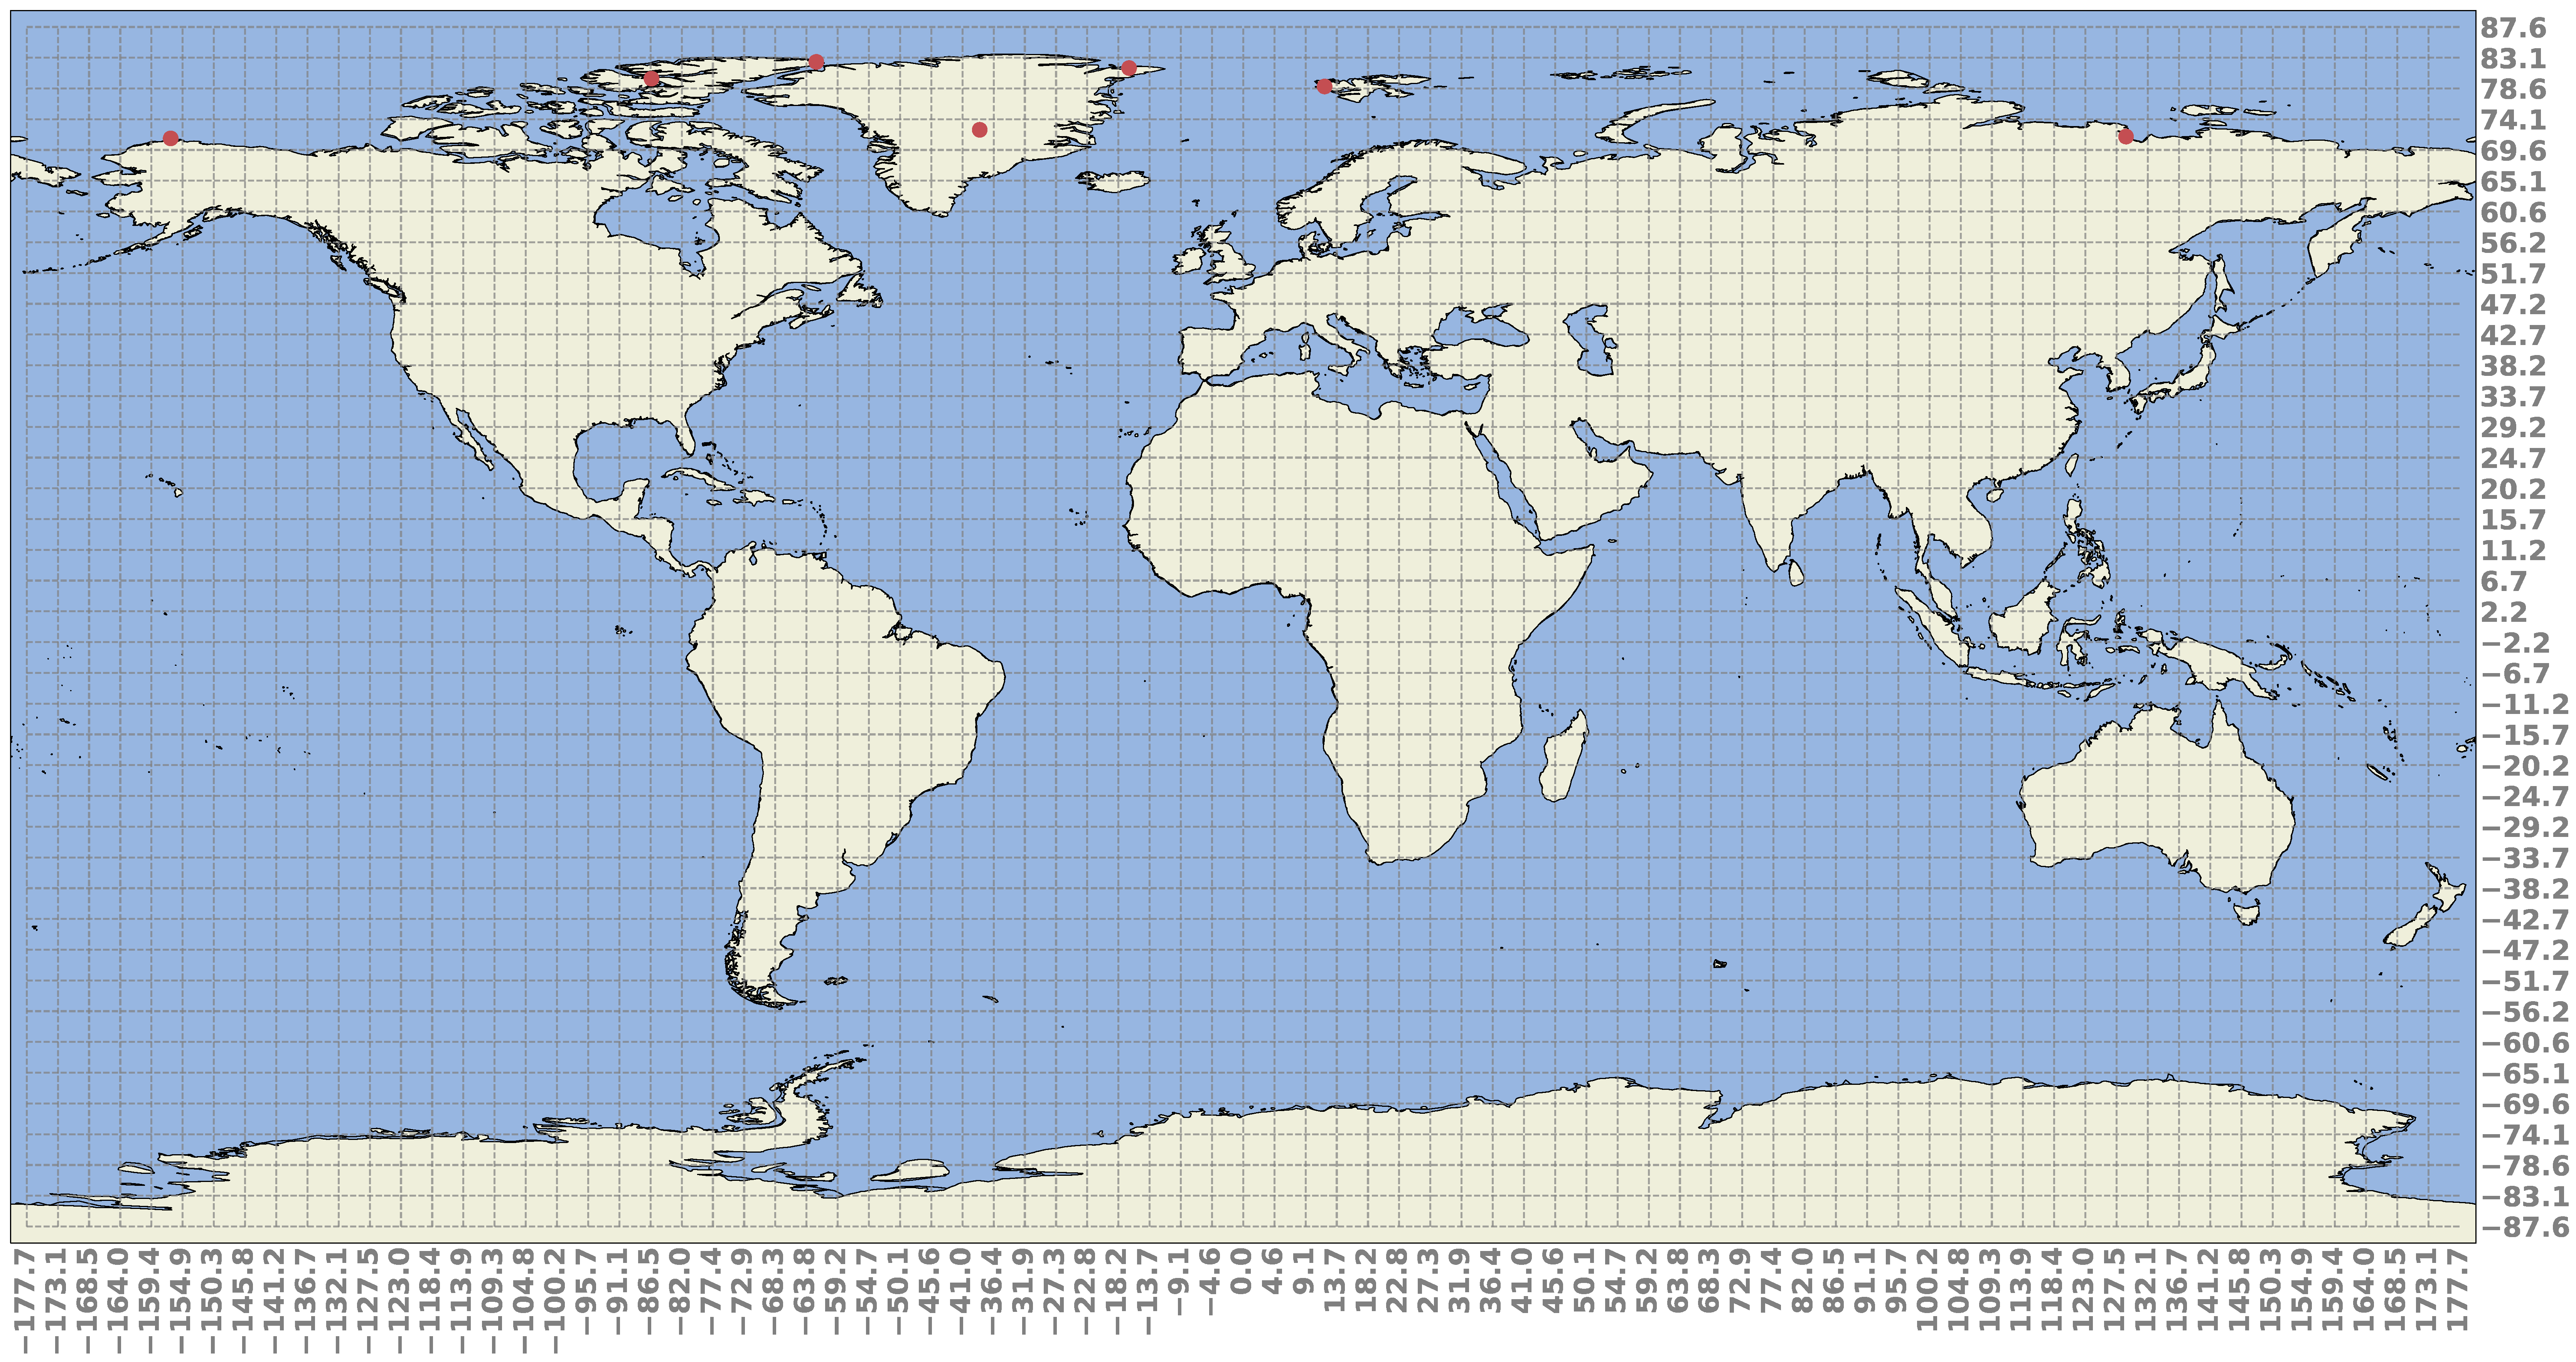
\includegraphics[width = \linewidth]{Appendix/images/resolution_map.pdf}
    \caption{Illustration of the grid coverage in the Oslo CTM3 globally at \texttt{HFOUR} $=$ 4.5$^o$x4.5$^o$ resolution. The red dots are the stations that were used for observational data}
    \label{fig:res_map_global}
\end{figure}

\clearpage
\section{Supporting Figures From Litterature}\label{app:supp_fig}

\begin{figure}
    \centering
    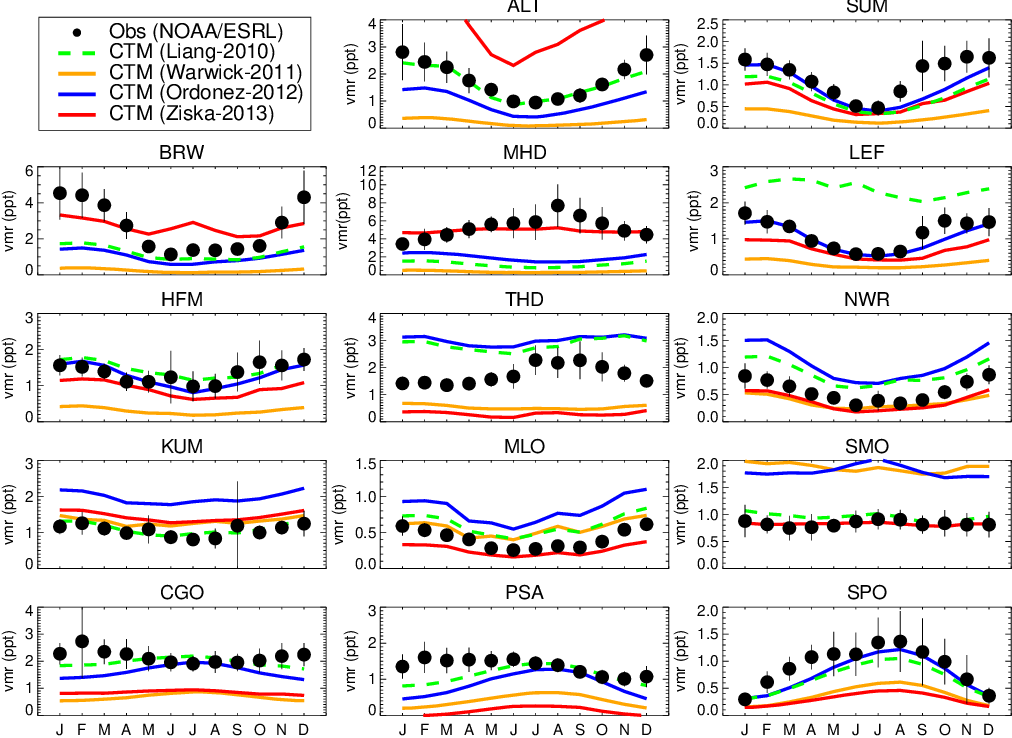
\includegraphics[width =0.7\linewidth]{Appendix/images/Hossaini2013_fig5_bromoform.png}
    \caption{Comparison of monthly mean mixing ratio (ppt) of $\chem{CHBr_3}$ output from \cite{Liang2010}, \cite{ziska}, warwick 2011, ordonez 2012}
    \label{fig:Hosaini_fig5}
\end{figure}

\begin{figure}
    \centering
    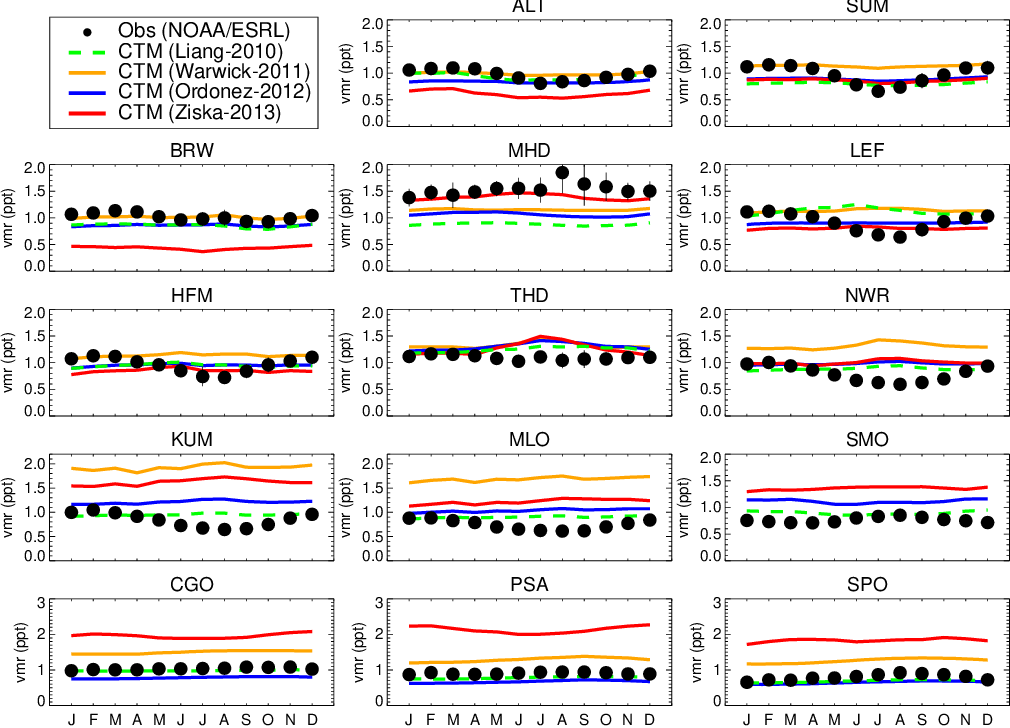
\includegraphics[width =0.9\linewidth]{Appendix/images/Hossaini2013_fig6_ch2br2.png}
    \caption{Comparison of monthly mean mixing ratio (ppt) of $\chem{CH_2Br_2}$ output from \cite{Liang2010}, \cite{ziska}, \cite{Warwick2006} and \cite{Ordonez2012}. The figure is adapted from \cite{Hossaini2013}}
    \label{fig:Hosaini_fig6}
\end{figure}


\begin{figure}[h]
    \centering
    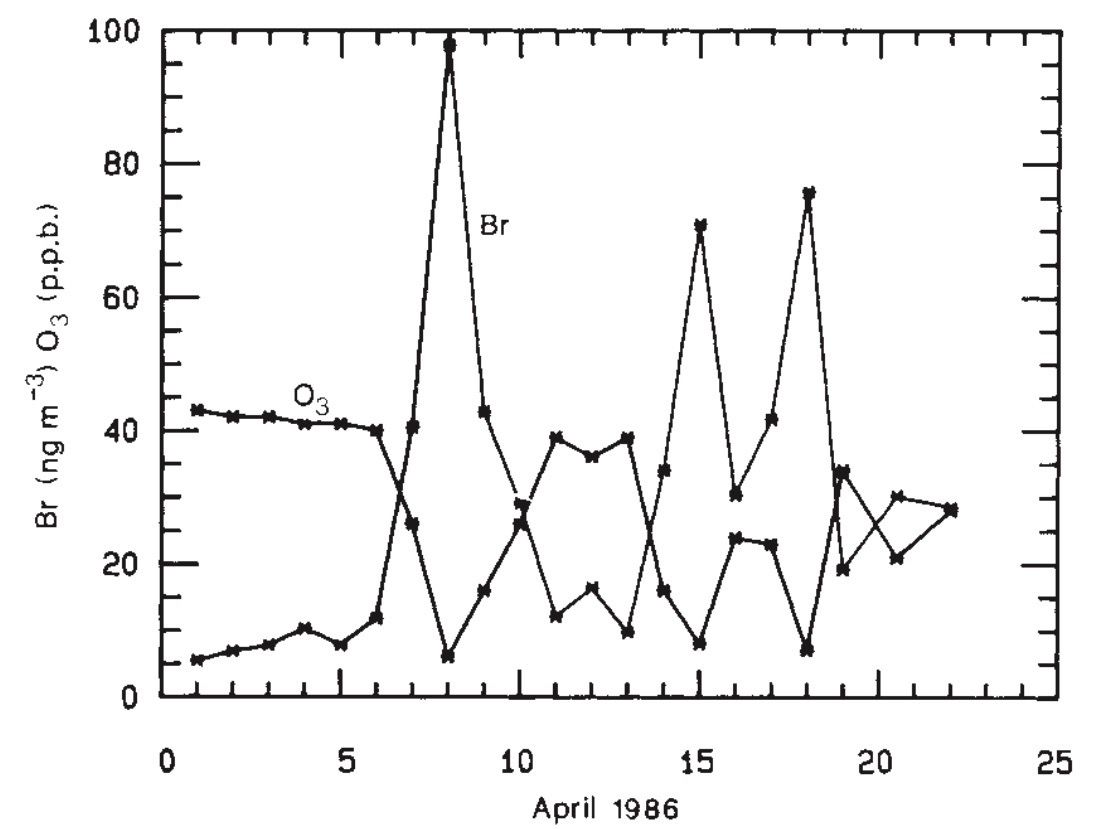
\includegraphics[width =0.8\linewidth]{Appendix/images/Barrie_1988.jpeg}
    \caption{Daily mean ground level $\chem{O_3}$ and filterable \chem{Br} (\chem{f-Br}) concentrations at Alert, Canada in April 1986. The figure is adapted from \cite{barrie}}
    \label{fig:Barrie_1988}
\end{figure}

\begin{figure}
    \centering
    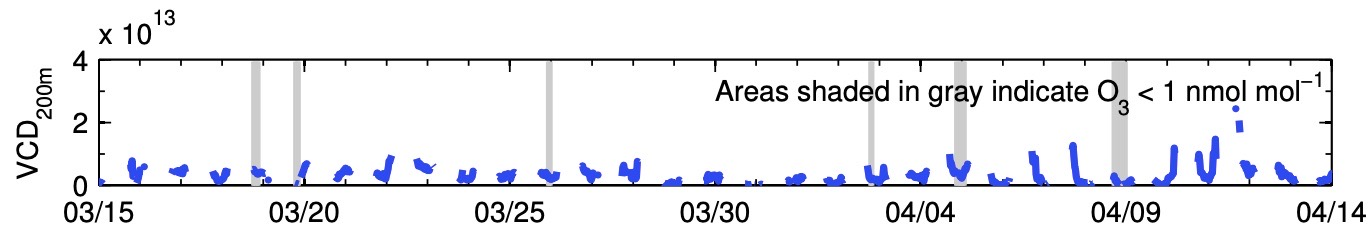
\includegraphics[width =0.9\linewidth]{Appendix/images/Peterson_2015.jpeg}
    \caption{\acrlong{vcd} ($molecules cm^{-2}$) of \chem{BrO} in the lowermost 200 m of the troposphere observed at Barrow, Alaska in 2012. The figure is adapted from \cite{Peterson2015}.}
    \label{fig:Peterson_2015}
\end{figure}

\cleardoublepage

\chapter{EBAS and NOAA Data}\label{app:ebas_noaa_data}


\section{Station Data}

Some key information about the station data obtained from ebas (\cite{EBAS}) is listed in Table \ref{tab:ebas_noaa_data_taken}. The chloride- and bromide- data were compared to the \chem{HBr}- and \chem{HCl}-concentration modelled as the measurements refers to filterable \chem{HBr} (the sum of particulate bromide and \chem{HBr} in the gas-phase). According to \cite{barrie}, these measurements contain about 50-93\% \chem{HBr}. 

\begin{table}[ht]
\centering
\resizebox{14cm}{!}{%
\begin{tabular}{|lllllll|}
\hline
\textbf{Station}  & \textbf{Variable}  & \textbf{Temporal res.} & \textbf{Timzone} & \textbf{Unit}  & \textbf{Instrument type} & \textbf{Year} \\ \hline
Alert            & $\chem{O_3}$ & 1h           & UTC              & $\mu$gm$^{-3}$  & uv\_abs                  & 2001               \\
Alert            & \chem{Cl}    & 1w           & UTC              & $\mu$gm$^{-3}$  & high\_vol\_sampler       & 2001, 2013         \\
Alert            & \chem{Br}    & 1w           & UTC              & $\mu$gm$^{-3}$  & high\_vol\_sampler       & 2001, 2013         \\
Barrow           & $\chem{O_3}$ & 1h           & UTC              & nmol/mol        & uv\_abs                  & 2001, 2013, 2018   \\
Eureka           & $\chem{O_3}$ & 1h           & UTC              & nmol/mol        & uv\_abs                  & 2018               \\
Summit           & $\chem{O_3}$ & 1h           & UTC              & nmol/mol        & uv\_abs                  & 2001, 2013, 2018   \\
Tiksi            & $\chem{O_3}$ & 1h           & UTC              & nmol/mol        & uv\_abs                  & 2013, 2018         \\
Villum           & $\chem{O_3}$ & 1h           & UTC              & $\mu$gm$^{-3}$  & uv\_abs                  & 2013               \\
Villum           & \chem{Cl}    & 1w           & UTC              & $\mu$gm$^{-3}$  & filter\_3pack            & 2013, 2017         \\
Villum           & \chem{Br}    & 1w           & UTC              & $\mu$gm$^{-3}$  & filter\_3pack            & 2017               \\
Zeppelin         & $\chem{O_3}$ & 1h           & UTC              & $\mu$gm$^{-3}$  & uv\_abs                  & 2001, 2013, 2018   \\ \hline
\end{tabular}
}
\caption{Key information about data taken from the different stations (\cite{EBAS}). The arithmetic mean value was used from all datasets. The temporal resolution, timezone and unit were given by each dataset. uv\_abs refers to the ultraviolet absorption method (For more information, see e.g. \cite{Galbally2013}). high\_vol\_sampler and filter\_3pack. The years were chosen according to when the model simulations were planned}
\label{tab:ebas_noaa_data_taken}
\end{table}


\section{Ozonosonde Data}

Ozonosonde measurements from Summit, Greenland, was obtained from \cite{NOAA} for the year 2013. The ozonosonde measures ozone by using an Electrochemical Concentration Cell Ozonosonde (For more information, visit \cite{ESRL}).  

\cleardoublepage

\chapter{Running the CTM3}\label{app:running_CTM3}

\section{The Supercomputer}\label{app:supercomputer}

\subsection{The Job File}

The job file is used to set up a run. The job file declares the job name, the input file, the project number and the wall clock limit, i.e. the max running time in the super computer and the number of nodes to use on the supercomputer when running the simulation. Also, it contains the path to the restart files (information about restart files can be found in Section \ref{subsec:restart_files}).

\subsubsection{Abel vs. Saga}

As the Oslo CTM3 was not optimized for Saga, the job file setup at Saga and Abel differed slightly. At Abel, the most efficient setup was the following: 

\begin{lstlisting}
#!/bin/bash
# Script for running on Abel.
# ----------------------------------------------
# Job name (enter your distinct job name):
#SBATCH --job-name=C3RUN_almost_BE
#
# Project (enter your noturn project number):
#SBATCH --account=geofag
#
# Wall clock limit (setting for one year 96:0:0):
#SBATCH --time=0:30:0
#
# Does your job exceed one week, use "--partition=long":
# ####SBATCH --partition=long
#
# Max memory usage:
#SBATCH --mem-per-cpu=3000M
#
# Number of cores:
#SBATCH --ntasks-per-node=16
#
# Number of nodes:
#SBATCH --nodes=1
#
#
## Set up job environment
source /cluster/bin/jobsetup
\end{lstlisting}

The number of nodes had to be different at Saga as it was slowed down by an increased number: 

\begin{lstlisting}
#!/bin/bash
# Script for running on Saga.
# ----------------------------------------------
# Job name (enter your distinct job name):
#SBATCH --job-name=C3RUN_BE_PI_HFOUR_MarchMay_2013
#
# Project (enter your noturn project number):
#SBATCH --account=nn9188k
#
# Wall clock limit (setting for one year 96:0:0):
#SBATCH --time=15:0:0
#
# Does your job exceed one week, use "--partition=long":
# ####SBATCH --partition=long
#
# Max memory usage:
#SBATCH --mem-per-cpu=3000M
#
# Number of cores:
#SBATCH --ntasks=1
#SBATCH --cpus-per-task=8
#
# Number of nodes:
#SBATCH --nodes=1
#
#
## Set up job environment:
#set -o errexit  # Exit the script on any error
set -o nounset  # Treat any unset variables as an error
\end{lstlisting}


\subsection{The Input File}

The input file consists of three parts, one that sets up the meteorological year, start day and end day. The second part lists some of the input file names, including the tracer lists. Information of the tracer list used here can be found in Section \ref{subsubsec:Ltracer_list} and \ref{subsubsec:tracer_list}. The third part covers information about the diagnostics. 

\medskip

In order to save CPU time and avoid conflicts regarding the use of stratospheric methyl bromide ($\chem{CH_3Br}$) as a designated species for $\chem{CHBr_3}$ and $\chem{CH_2Br_2}$ (explained further in Section \ref{sec:oceanic_emissions}), the stratosphere was turned off. How this was performed is explained in Section \ref{app:turning_off_the_stratosphere}.

\medskip

In the Pre-industrial setups are slightly different and explained in Section \ref{app:PI_run}

\section{Emission List - \texttt{Ltracer\_emis\_ceds17\_YEAR\_megan.d}}
\label{subsubsec:Ltracer_list}

The tracer list contains all the emission information that the model needs to be able to run. The emission inventory used in this thesis is the \acrlong{ceds} inventory and the \acrlong{megan}, version 2.10, inventory. 

\medskip

\acrshort{ceds} is a historical emission inventory for anthropogenic aerosol and precursor compounds (\cite{Lund2018}). The historical emissions are only available for the 1750-2014 period, which limits the possibilities for simulations after 2014 in this thesis. 

\medskip

\acrshort{megan} v2.10 is a framework used by the model to estimate biogenic fluxes between terrestrial ecosystems and the atmosphere (\cite{Guenther2012}). 



\section{Tracer List - \texttt{tracer\_list\_no\_stratosphere.d}}\label{subsubsec:tracer_list}

The tracer list contains all the tracers that the model need in the simulation, with names and molecular weights. It contains two parts - one with transported species and one with non-transported species. The total number of transported and non-transported must match the \texttt{NPAR} and \texttt{NOTRPAR} in \texttt{cmn\_size.F90} (see Section \ref{subsubsec:cmn_size}) (\cite{SovdeManual}). 

\medskip

The list \texttt{tracer\_list\_no\_stratosphere.d} was created in order to include some of the stratospheric chemistry components as well as the components mentioned above. The added components were: 

\begin{itemize}
    \item \textbf{Transported}: $\chem{Cl_x}$, $\chem{HCl}$, $\chem{Cl_y}$, $\chem{CH_3Br}$, $\chem{Br_y}$, $\chem{ClO}$, $\chem{Cl_2}$, $\chem{HBr}$, $\chem{BrONO_2}$, $\chem{OHBr}$, $\chem{Br_2}$, $\chem{BrCl}$, $\chem{Cl}$, $\chem{Br}$, $\chem{BrO}$
    \item \textbf{Non-transported}: $\chem{H_2}$
\end{itemize}

The three components $\chem{Cl}$, $\chem{Br}$, $\chem{BrO}$ were moved from non-transported in the \texttt{bromine\_explosion}-branches, in order to have transport for these species. They were left in non-transported in the \texttt{origCTM3\_noStrat}-branches, as the lack of chemistry for those species in the original CTM3-branches led to conflicts (for an overview of the branches, see Section \ref{sec:code_availability}). 




\section{Restart Files}\label{subsec:restart_files}


The restart file is a NetCDF file that contains the tracer distribution and moments for all species in a simulation. For the transported species, it has prefix \texttt{STT}, and \texttt{XSTT} for the non-transported species. The transported species are associated with their moments, which has the prefixes \texttt{SUT}, \texttt{SVT}, \texttt{SWT}, \texttt{SUU}, \texttt{SVV}, \texttt{SWW}, \texttt{SUV}, \texttt{SUW}, \texttt{SVW} (\cite{SovdeManual}). The restart file is used as an initial field for the production run, which requires a spin up, and it is therefore necessary to determine the length of the spin up (in model time) according to the lifetime of the chemical species of interest. 

\medskip

Restart files used in \cite{Falk_2019} was provided by Stefanie (\texttt{ctm3\_restart\_20010101.nc}) and used for my own spin-up. The provided restart file was spun-up over a 10 years transient run starting in 1990. It was necessary to make new restart files, as the code is changed and the stratosphere is turned off, which alters the chemistry. The restart files were thus based on the same emission inventory (MEGAN and CEDS17) except for biomass burning which was taken from CEDS17 instead of GFed. The reason for this is that the GFed files only exist until 2005, and my intent was to run the model in later years as well. 

\medskip


The dry-deposition scheme also differs, where I have used the old dry-deposition scheme instead of the mOSaic scheme (for more information, see \cite{Falk_2019} and references therein). The main difference between the dry-deposition schemes is that the dry deposition rate in the old scheme is lower over ice and snow surfaces, leading to a general overestimation of $\chem{O_3}$.


\medskip

The spin-up time is the time it takes for the simulated surface concentrations to be unaffected by initial conditions. \cite{Curci_AirPollution} found that the optimal model spin-up time in terms of ozone was 9 days. Although this study was based on a domain in the GEOS-Chem global model and a regional model, and had a different set-up than the Oslo CTM3, this estimate is applicable to my own spin-up. It also stated by \cite{SeinfeldSpyros} that the global mean lifetime of tropospheric ozone is 19 days. In order to be sure that the chemistry is indeed spun up properly, the restart files were ran for 3 months. 

\subsection{Pre-Industrial and Present-Day Restart Files}\label{sec:PI_and_PD_restart}

The pre-industrial and present-day restart files were made without moving the tracers \chem{Br}. \chem{BrO} and \chem{Cl} to transported species (for information about moving species from non-transported to transported, see Section \ref{subsubsec:tracer_list}). This became the solution to the problem that the original versions of the CTM3 (i.e. unaltered except for turning off the stratosphere in both cases and downscaling of the methane field in the case of the \acrshort{pi}-runs) had problems running. As there is no handling of these non-transported tracers in the troposphere in these branches. 

\cleardoublepage

\chapter{Turning Off the Stratosphere}\label{app:turning_off_the_stratosphere}

In order to save CPU time and avoid conflicts regarding the use of stratospheric methyl bromide ($\chem{CH_3Br}$) as a designated species for $\chem{CHBr_3}$ and $\chem{CH_2Br_2}$ (explained further in Section \ref{sec:oceanic_emissions}), the stratosphere was turned off. This is performed by modifying the following scripts: 

\section{Makefile}\label{subsubsec:makefile}

\texttt{Makefile} is the file that sets the user options for the CTM3. The resolution was either set to \texttt{HTWO} (2.25$^o$x2.25$^o$) or \texttt{HFOUR} (4.5$^o$x4.5$^o$). The following modules were also turned on or off (information about the different modules can be found in \cite{SovdeManual}):

\begin{itemize}
    \item \texttt{OSLOCHEM}: compilation with Oslo chemistry/physics, \textbf{turned on}
    \item \texttt{TROPCHEM}: compilation with Oslo tropospheric chemistry, \textbf{turned on}
    \item \texttt{STRATCHEM}: compilation with Oslo stratospheric chemistry, \textbf{turned off}
    \item \texttt{SULPHUR}: sulfur scheme, \textbf{turned on}
    \item \texttt{BCOC}: black carbon/organic matter scheme, \textbf{turned off}
    \item \texttt{NITRATE}: nitrate scheme (\texttt{SALT} and \texttt{SULPHUR} is required), \textbf{turned on}
    \item \texttt{SEA SALT}: sea salt scheme, \textbf{turned on}
    \item \texttt{DUST}: dust scheme, \textbf{turned off}
    \item \texttt{SOA}: secondary organic aerosols scheme, \textbf{turned off}
    \item \texttt{E90}: applies e90 tracer for STE flux calculations and produces the troposphere, \textbf{turned off}
    \item \texttt{LINOZ}: applies Linoz $\chem{O_3}$ for STE calculations (not set up yet to replace stratospheric chemistry in the Oslo CTM3), \textbf{turned off}
    \item \texttt{M7}: not implemented \textbf{turned off}
\end{itemize}


\section{Tropospheric Chemistry Parameters - \texttt{cmn\_size.f90}}\label{subsubsec:cmn_size}


The tropospheric chemistry parameters were adjusted in \texttt{cmn\_size.f90} in order to be able to include some of the originally stratospheric tracers without including the stratosphere. This was only done for the \texttt{bromine\_explosion}-branches (An overview of the branches can be seen in Section \ref{sec:code_availability}). 

\medskip

The non-transported species (\texttt{NPAR\_TROP}) were adjusted from 39 to 54 and the transported species (\texttt{NOTRPAR\_TROP}) were adjusted from 7 to 8 leaving the following amount of chemical parameters:

\begin{itemize}
    \item \texttt{TROPCHEM}: 54 transported, 8 non-transported
    \item \texttt{SULPHUR}: 5 transported
    \item \texttt{NITRATE}: 5 transported
    \item \texttt{SEA SALT}: 8 transported
\end{itemize}

The numbers of transported- and non-transported species must match the number of these species in the tracer list (see Section \ref{subsubsec:tracer_list}) 


\section{Component Output - \texttt{gmdump3hrs.f90}}\label{subsubsec:gmdump}

In the module \texttt{gmdump3hrs.f90}, selected tracer components are printed every hour. In this module, the tracer output was adjusted to dump 19 components instead of 7. To be able to do this, the components must be declared as "transported" in the tracer list (Described in Section \ref{subsubsec:tracer_list}) and in \texttt{cmn\_size.F90} (Described in Section \ref{subsubsec:cmn_size}).


\cleardoublepage

\chapter{Pre-Industrial Run}\label{app:PI_run}


The model was run with pre-industrial emissions, taken as the year 1850 in this thesis (\cite{IPCCchapter8}). In order to set up the CTM3 for this, a few steps has to be changed. Keep in mind that the approach was hard-coded in order to avoid having to make a 9 years spin up in the restart-file (due to the atmospheric lifetime of methane). 

\medskip

The tracer list,  \texttt{Ltracer\_emis\_ceds17\_1850\_megan.d}, was set for 1850. 

\medskip

In \texttt{ch4routines.f90}, the subroutine \texttt{ch4surface\_scale\_hymn} was activated along with \texttt{ch4surface\_hymn}, allowing scaling of the methane-surface field with 1850 values, taken as 808.25 ppm (value suggested by \cite{RagnhildPersonal}). The scaling was hard-coded to this value. 

\medskip

The subroutine \texttt{set\_ch4\_stt} (also in \texttt{ch4routines.f90}) was activated from \texttt{pmain.f90} to allow scaling of the entire field (lev, lon and lat) (not only the surface field). 

\cleardoublepage

\chapter{Chemical Unit Conversion}

The following appendix contains the conversion procedures concerning the CTM3 output as well as the conversion of station data to a mass mixing ratio. When analysing atmospheric data such as gases, it is most appropriate to use the mixing ratio (mol mol$^{-1}$), or mole fraction, as it is not dependent on pressure and temperature as the concentration (mol m$^{-3}$) is. It is defined as the ratio of the amount (or mass) of the substance in a given volume to the total amount (or mass) of all constituents in that volume (\cite{SeinfeldSpyros}). 

\medskip

The first section contains the formulas applied to the CTM3 data and the EBAS/NOAA data. The second section contains the \acrfull{cdo} procedure, which is a procedure for processing \acrshort{netcdf}-files. 

\section{Chemical Unit Conversion}

\subsection{Oslo CTM3}\label{sec:unit_conversion_CTM3}

The CTM3 data used were given in either monthly averages or tropospheric tracers (3-hour outputs). The monthly averages have units kg of species, and the 3-hour outputs have units g m$^{-3}$. 

\medskip

To obtain the mixing ratio from the monthly averages, the following was applied:

\begin{equation}
    \chem{X_{VMR}} = \frac{\chem{M_{air}}}{\chem{M_{X}}}\frac{\chem{X_{kg}}}{\chem{air_{kg}}}
    \label{eq:vmr_monthly_avg}
\end{equation}

In which $\chem{X_{VMR}}$ is the volume mixing ratio of the species, $\chem{M_X}$ and $\chem{M_{air}}$ are the molecular masses of the species of interest and air. $\chem{X_{kg}}$ and $\chem{air_{kg}}$ are the output data from CTM3 in kg of species. 

\medskip

In order to change the units of the tropospheric tracers (3-hour output), the following was performed: 

\begin{equation}
    \chem{X_{VMR}} = \frac{\chem{M_{air}}}{\chem{M_{X}}}\frac{\chem{X_{ g/cm^{3}}}}{\chem{\rho_{air}}}
    \label{eq:vmr_trop_tracer}
\end{equation}

In which  $\chem{X_{\mu g/m^{3}}}$ is the concentration of the species and $\chem{\rho_{air}}$ is the density of air (in $\mu g/m^{3}$). These are the output data from CTM3.


\subsection{EBAS/NOAA}\label{sec:unit_conversion_EBASNOAA}

The EBAS and NOAA data were provided in units $\mu g m^{-3}$, and were thus changes by: 

\begin{equation}
    \chem{X_{VMR}} = \frac{\chem{M_X}}{\chem{M_{air}}}\frac{\chem{X_{\mu g/cm^{3}}}}{\chem{\rho_{air}}}
\end{equation}

Density of air was taken as 1.204 kgm$^{-3}$ (at 293.15 K). 


\section{Unit Conversion Using cdo}\label{sec:cdo}

The \acrshort{cdo}-software is a collection of operators for standard processing of climate and forecast data (\cite{cdo}). CDO is ideal for processing of large \acrshort{netcdf} datasets. 


\medskip

The \acrshort{cdo}-scripts were adapted from scripts provided by \cite{StefaniePersonal}. 



\begin{itemize}
    \item Load cdo by \texttt{module load cdo}
    \item \texttt{chmod +x "cdo file"} if there has been changes
    \item \texttt{./"cdo file" "Full path"} 
\end{itemize}


%\addcontentsline{toc}{chapter}{Appendix B: Additional figures}
\cleardoublepage

\chapter{Additional Results}\label{chap:add_res}

\section{CTM3 Developement}\label{app:CTM3_dev}

\begin{figure}[ht]
    \centering
    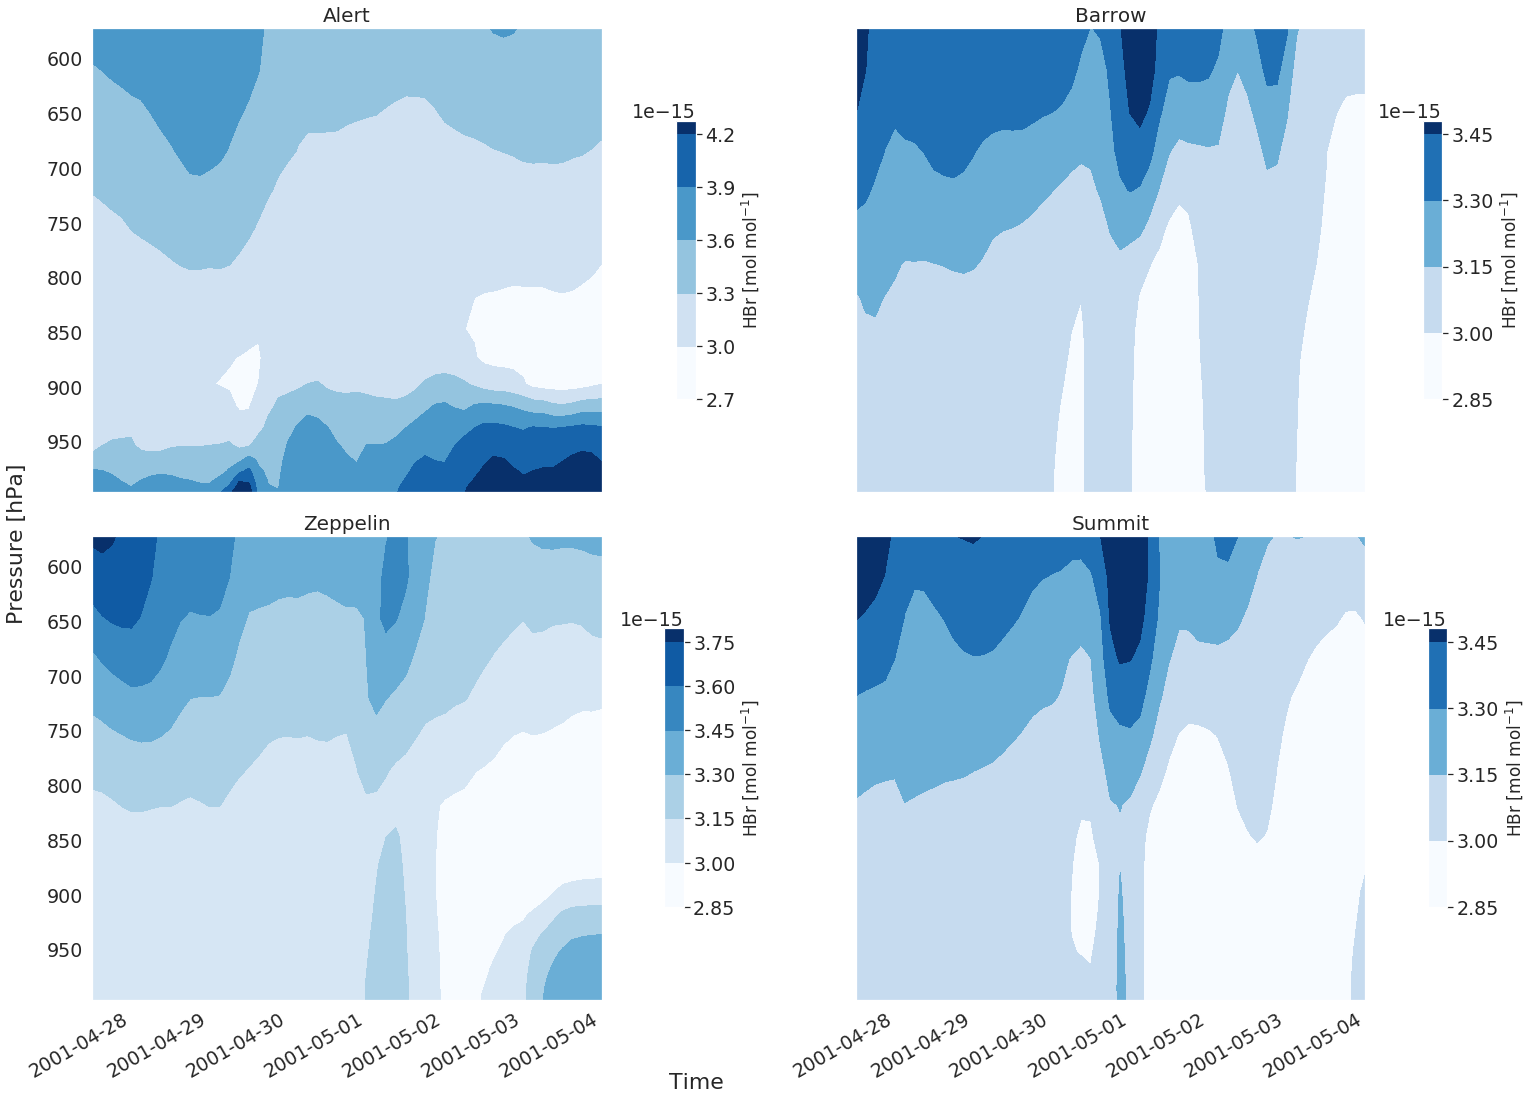
\includegraphics[width = \linewidth]{Chapter6_Results/images/Vert_StationComp_2001/vertHBr_noCl.png}
    \caption{Mixing ratio ($mol mol^{-1}$) of \chem{HBr} in the model layers up to $\sim 600 hPa$ at the four different stations Alert (top left), Barrow (top right), Zeppelin (lower left) and Summit (lower right) in April-May, 2001. The result is from Branch \ref{def:BE_PD_noCl}}
    \label{fig:vertHBr_noCl}
\end{figure}

\begin{figure}[h]
    \centering
    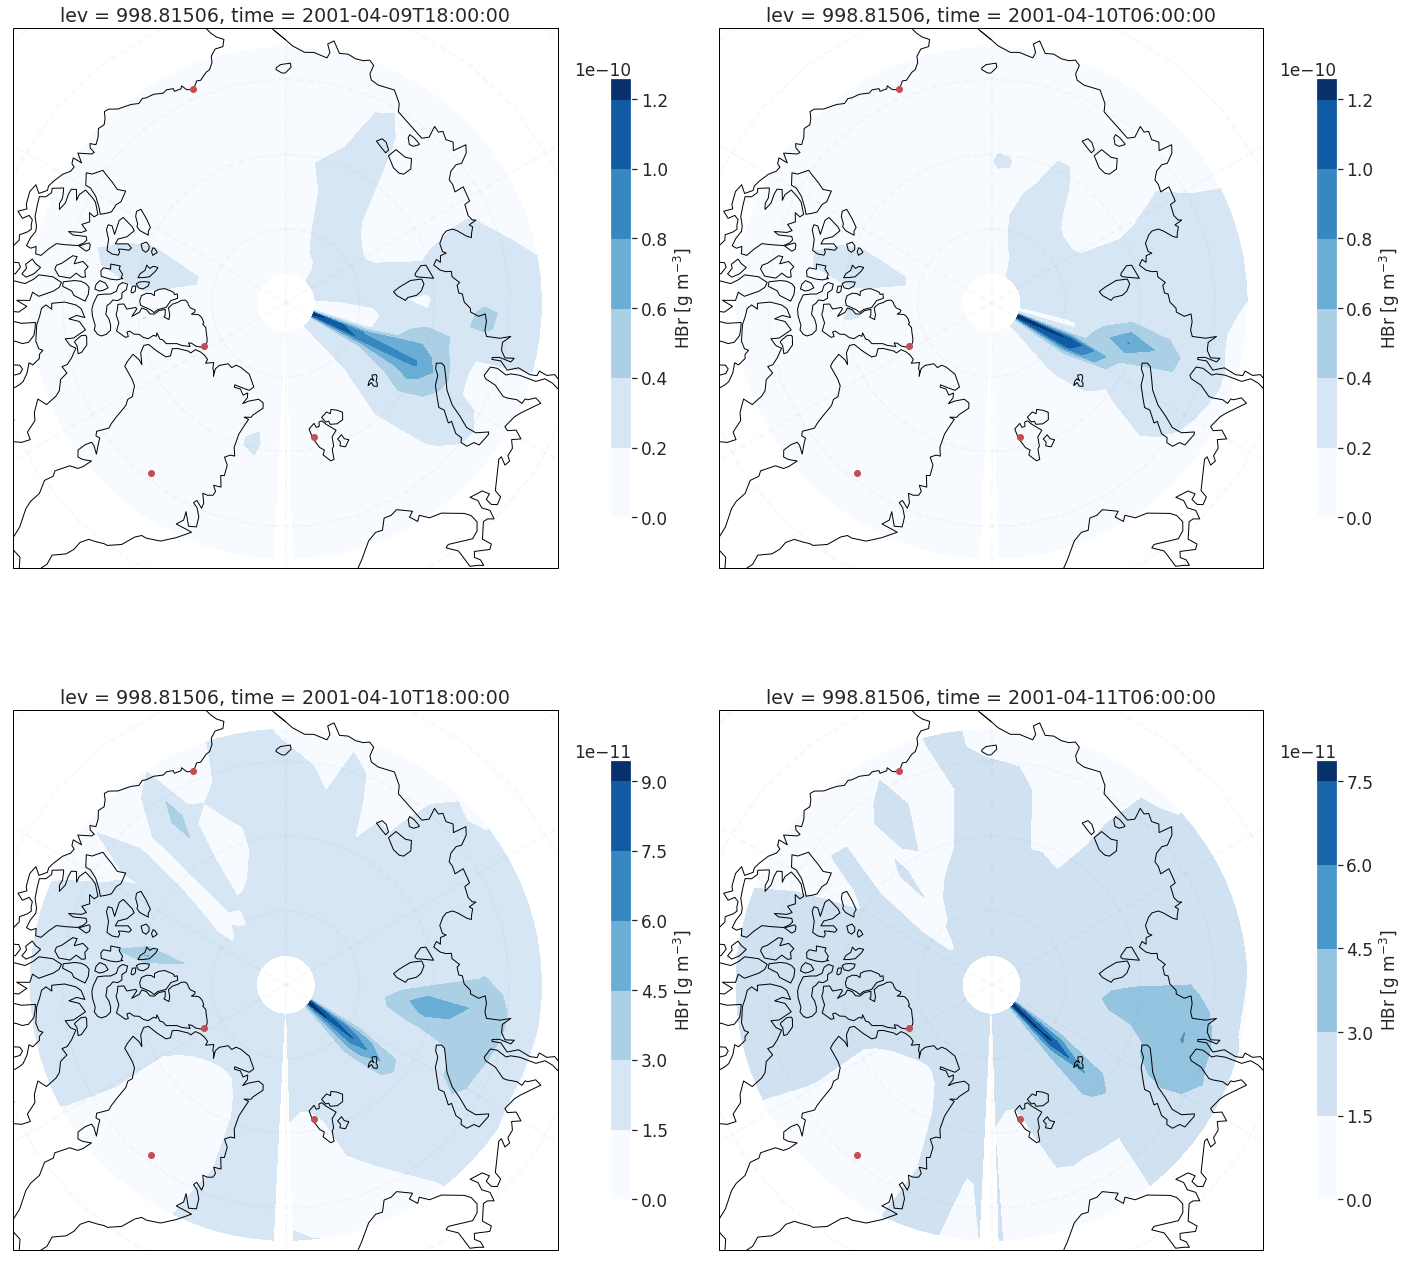
\includegraphics[width = \linewidth]{Chapter6_Results/images/Polar_StationComp_2001/HBr/polarHBr_noCl.png}
    \caption{Concentration ($g m^{-3}$) of \chem{HBr} in the first model layer the Arctic at 18:00 and 06:00 (UTC) of the 9th, 10th and 11th of April, 2001. The result is from Branch \ref{def:BE_PD_noCl} The red dots are the positions of the stations with observations in 2001 (see the map in Figure \ref{fig:stns} for reference)}
    \label{fig:polarHBr_noCl}
\end{figure}

\begin{figure}[h]
    \centering
    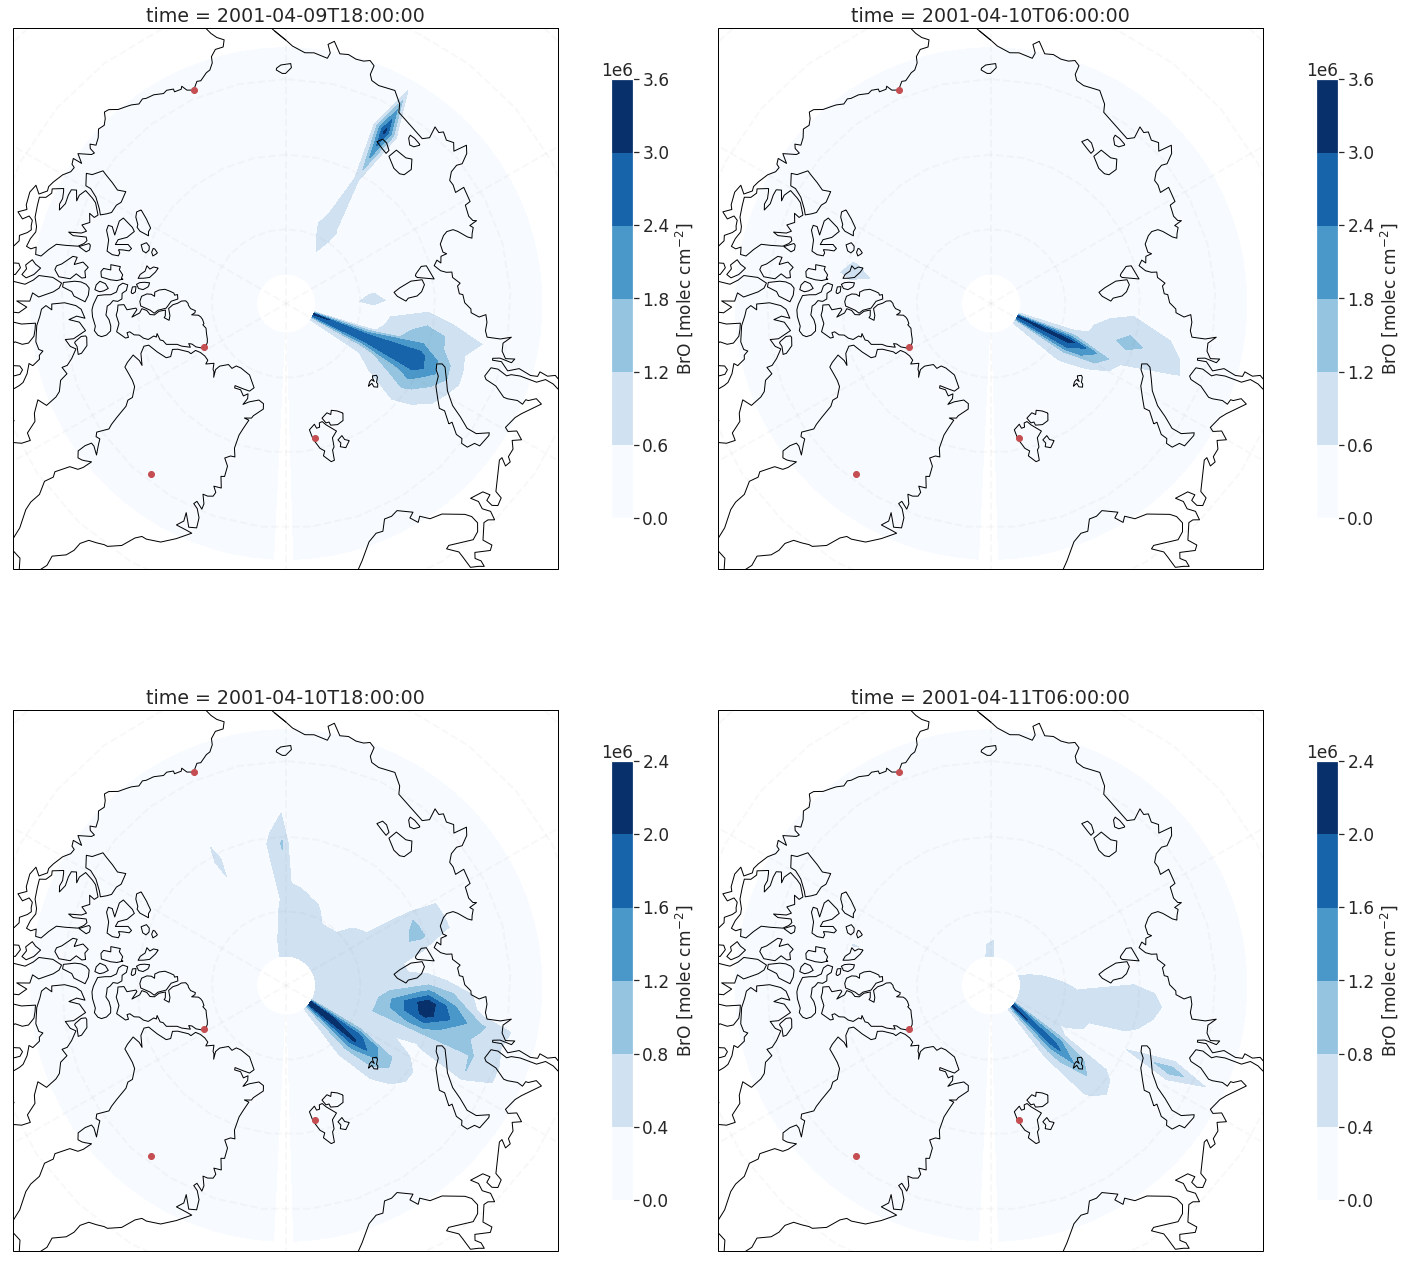
\includegraphics[width = \linewidth]{Chapter6_Results/images/Polar_StationComp_2001/BrO/polarBrO_noCl.png}
    \caption{Vertical column density ($molecules cm^{-2}$) of \chem{BrO} in the lowermost $\sim 250 m$ at 18:00 and 06:00 (UTC) on the 9th, 10th and 11th of April, 2001. The result is from Branch \ref{def:BE_PD_noCl}. The red dots are the positions of the stations with observations in 2001 (see the map in Figure \ref{fig:stns} for reference)}
    \label{fig:polarBrO_noCl}
\end{figure}

\begin{figure}[h]
    \centering
    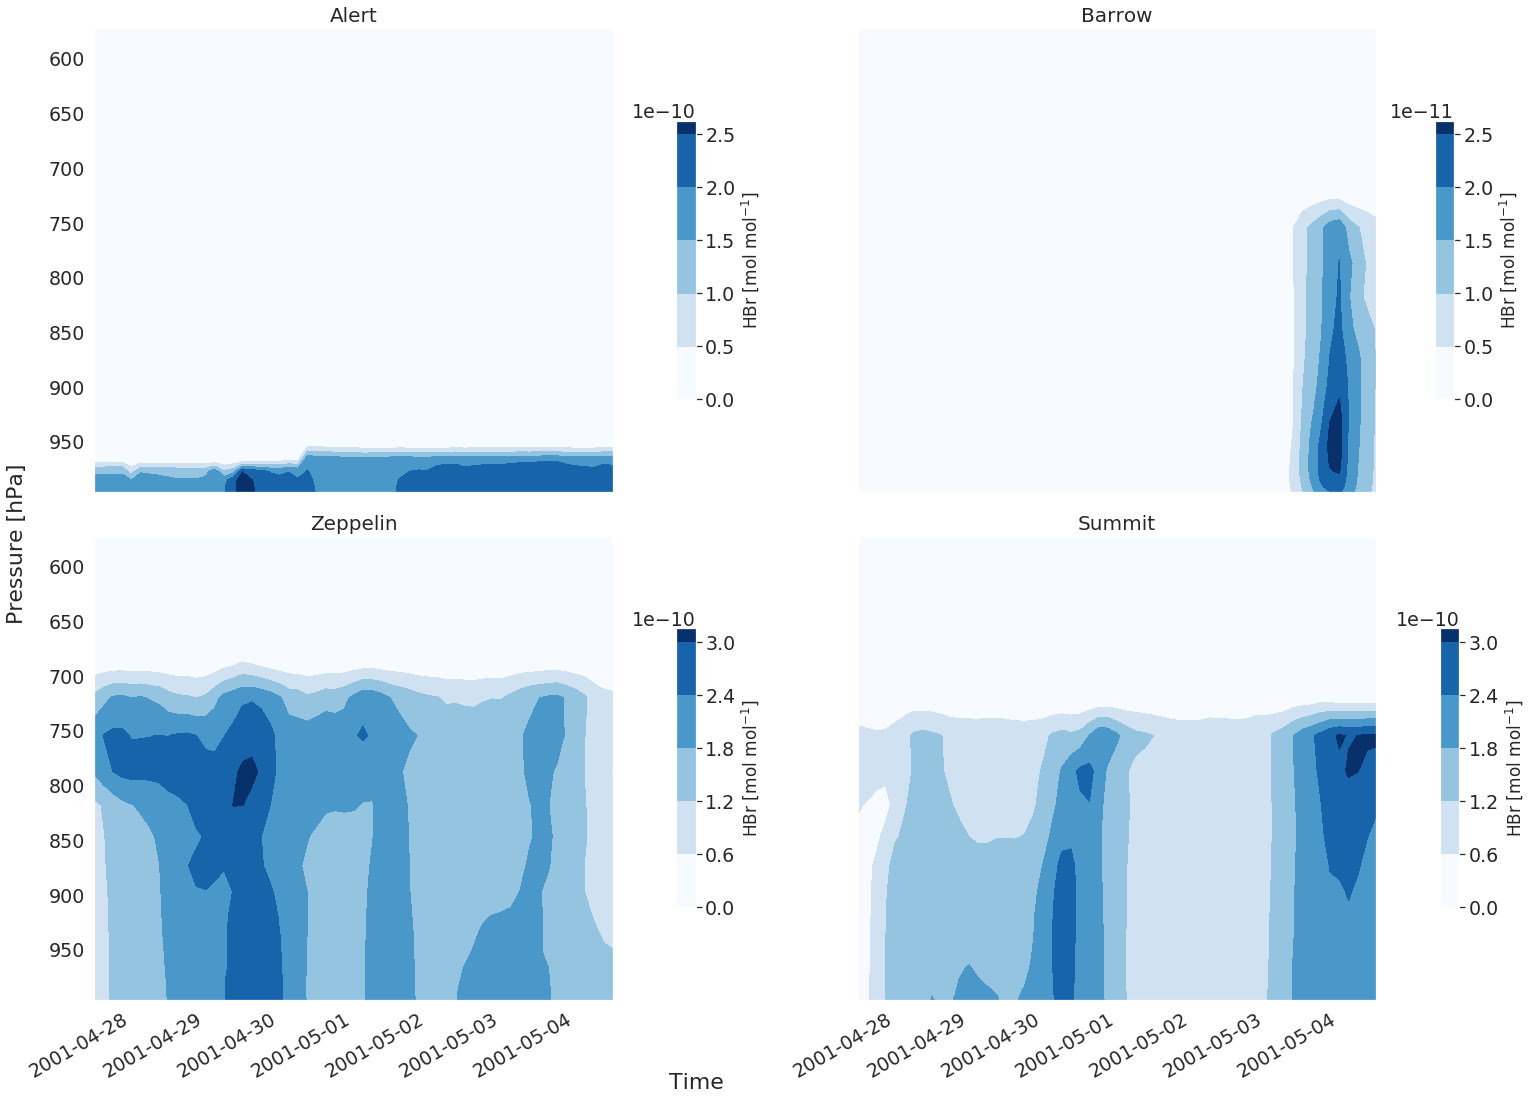
\includegraphics[width=\linewidth]{Chapter6_Results/images/Vert_StationComp_2001/vertHBr_newRestart.png}
    \caption{Mixing ratio ($mol mol^{-1}$) of \chem{HBr} in the model layers up to $\sim 600 hPa$ at the four different stations Alert (top left), Barrow (top right), Zeppelin (lower left) and Summit (lower right) in April-May, 2001. The result is from Branch \ref{def:BE_PD_noCl} initialized with a new restart file with a \chem{HBr} concentration of 10 ppt}
    \label{fig:vertHBr_newRestart}
\end{figure}

\begin{figure}[h]
    \centering
    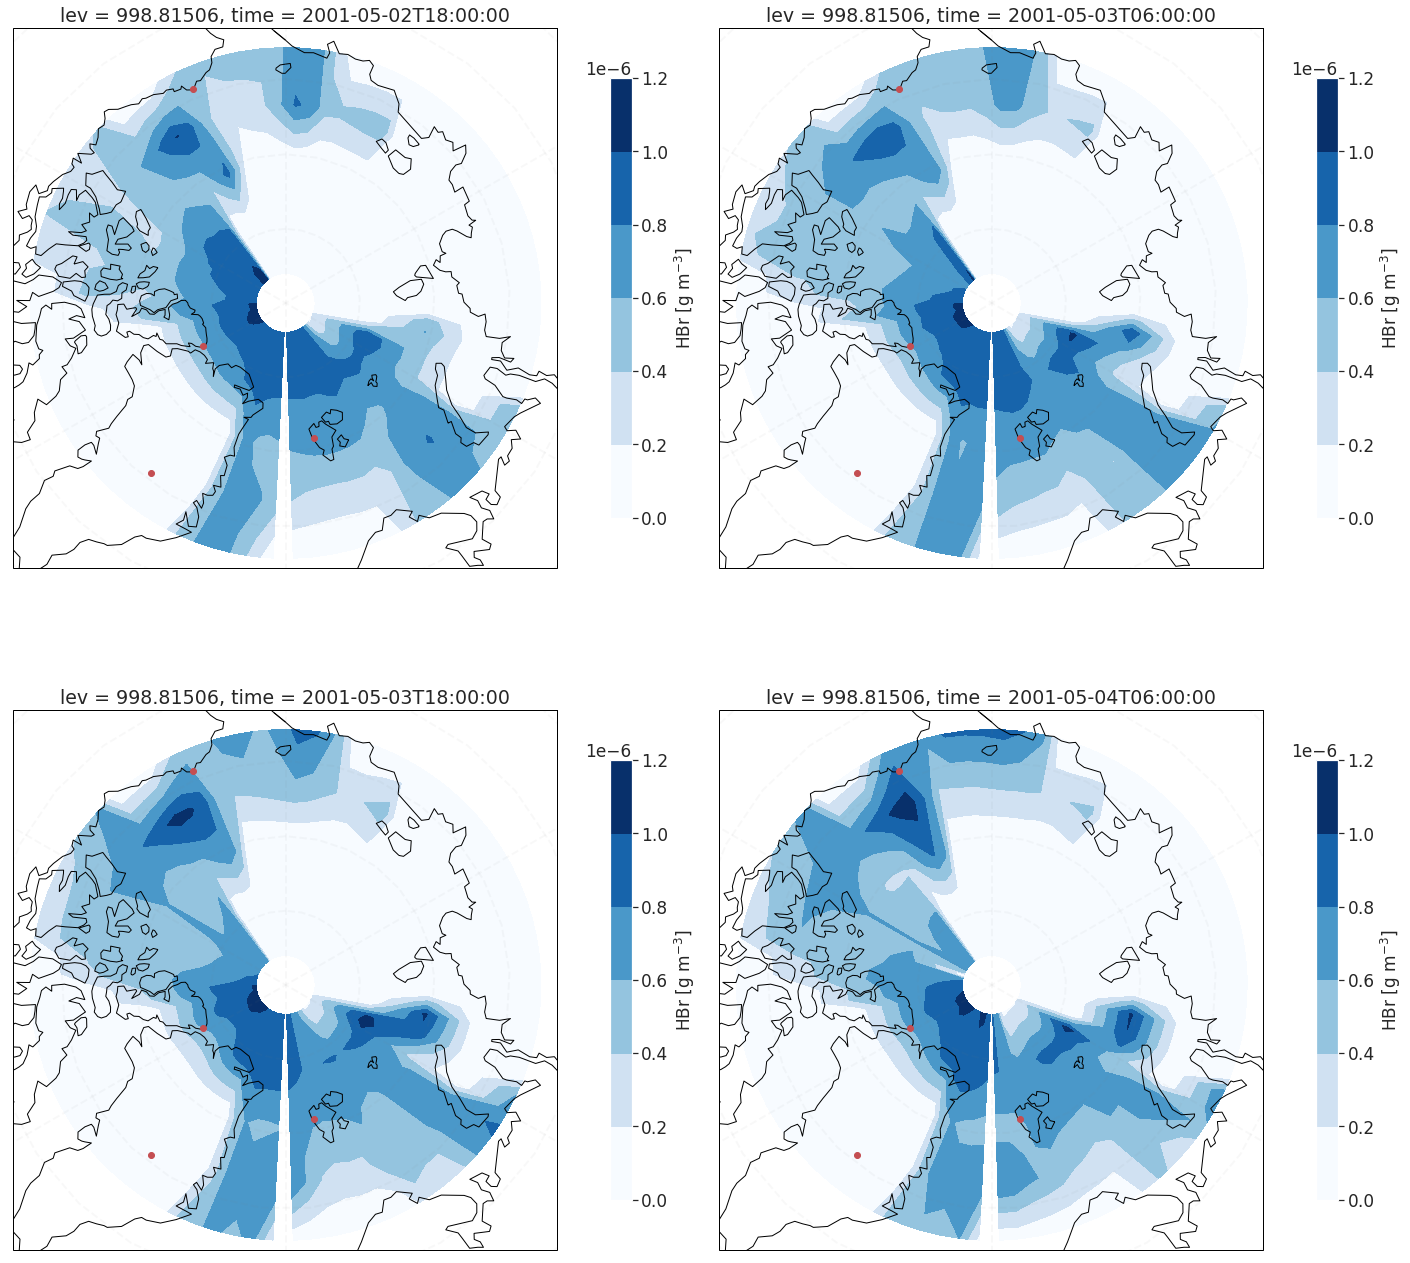
\includegraphics[width=\linewidth]{Chapter6_Results/images/Polar_StationComp_2001/HBr/polarHBr_newRestart.png}
    \caption{Concentration ($g m^{-3}$) of \chem{HBr} in the first model layer the Arctic at 18:00 and 06:00 (UTC) of the 2nd, 3rd and 4th of May, 2001. The result is from Branch \ref{def:BE_PD_noCl} initialized with a new restart file with a \chem{HBr} concentration of 10 ppt. The red dots are the positions of the stations with observations in 2001 (see the map in Figure \ref{fig:stns} for reference)}
    \label{fig:polarHBr_newRestart}
\end{figure}

\begin{figure}[h]
    \centering
    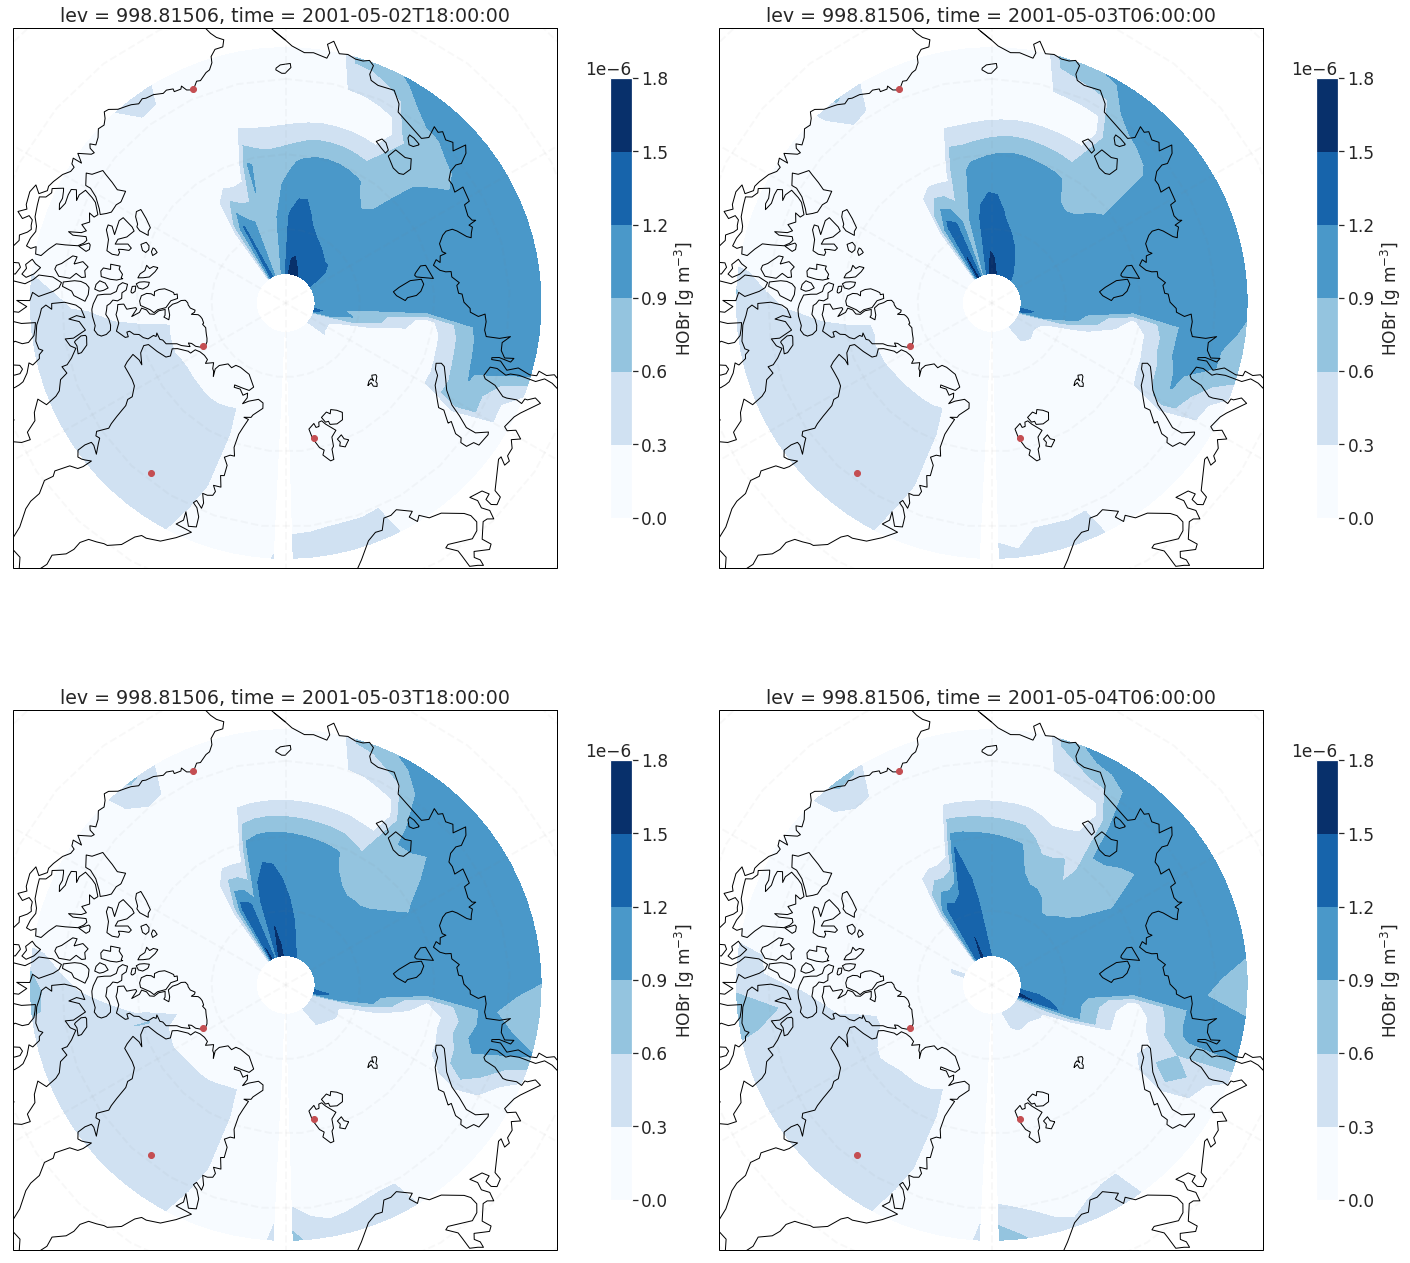
\includegraphics[width=\linewidth]{Chapter6_Results/images/Polar_StationComp_2001/HOBr/polarHOBr_newRestart.png}
    \caption{Concentration ($g m^{-3}$) of \chem{HOBr} in the first model layer the Arctic at 18:00 and 06:00 (UTC) of the 2nd, 3rd and 4th of May, 2001. The result is from Branch \ref{def:BE_PD_noCl} initialized with a new restart file with a \chem{HBr} concentration of 10 ppt. The red dots are the positions of the stations with observations in 2001 (see the map in Figure \ref{fig:stns} for reference)}
    \label{fig:polarHOBr_newRestart}
\end{figure}

\begin{figure}[h]
    \centering
    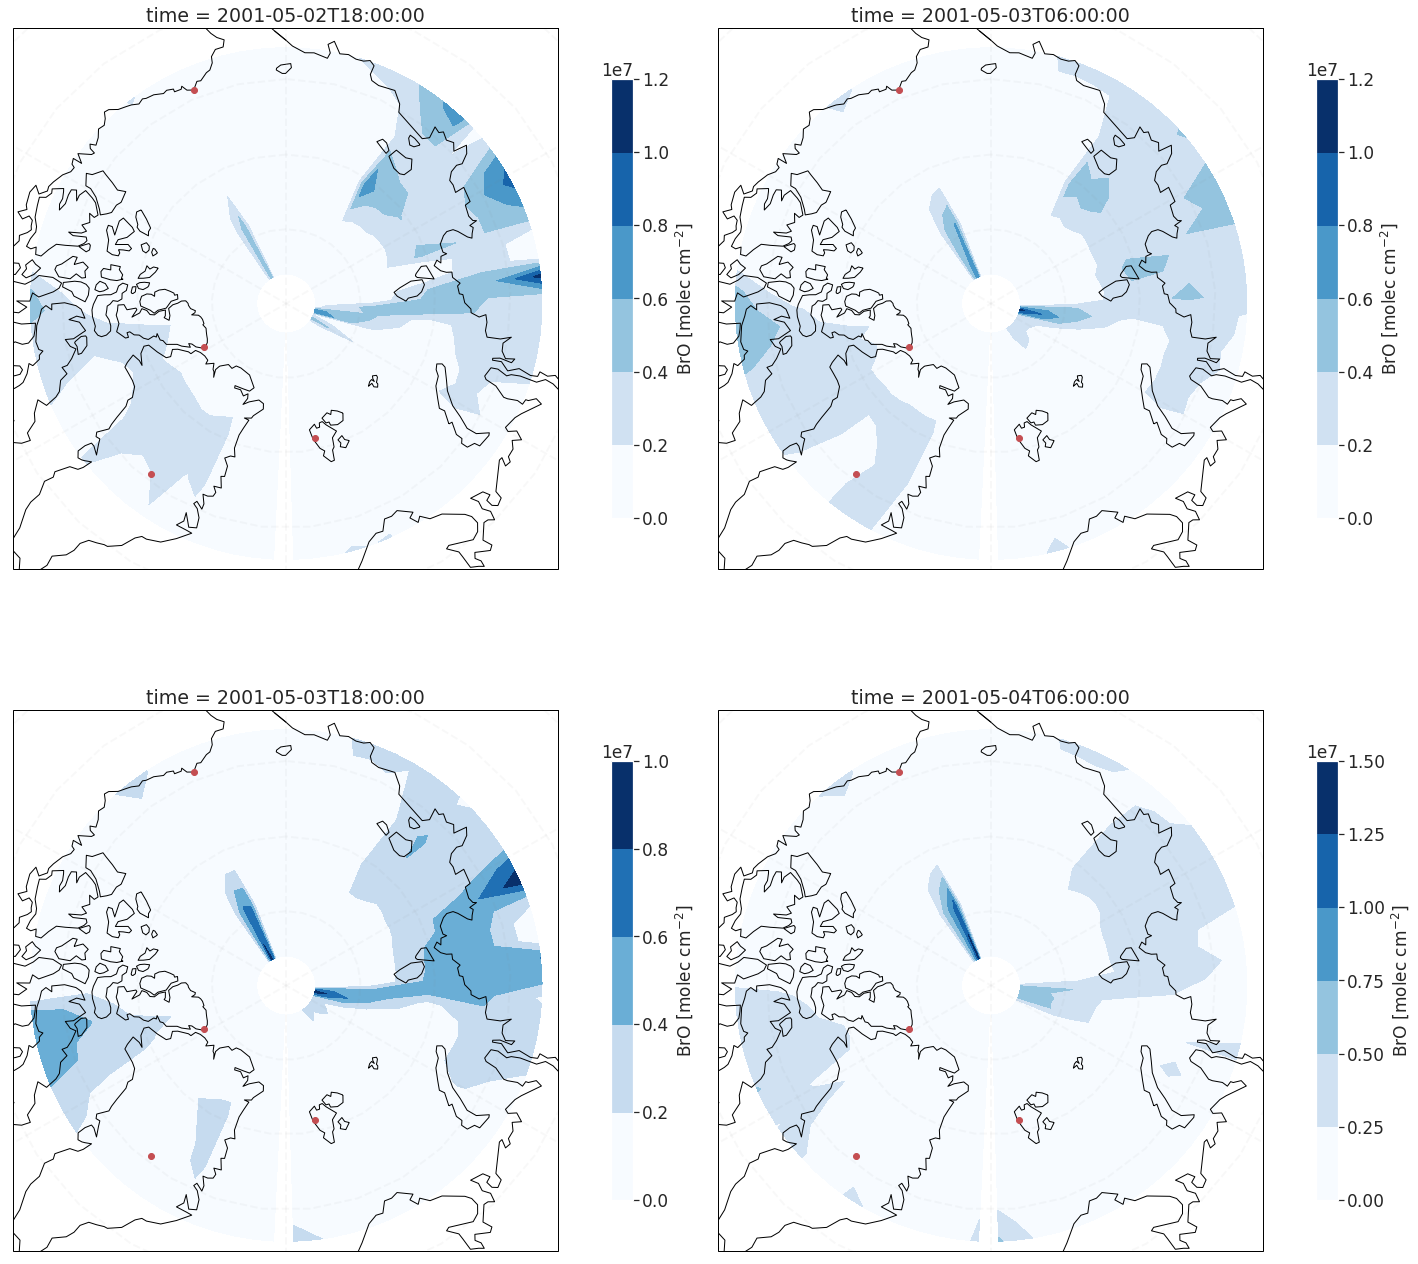
\includegraphics[width=\linewidth]{Chapter6_Results/images/Polar_StationComp_2001/BrO/polarBro_newRestart.png}
    \caption{Vertical column density ($molecules cm^{-2}$) of \chem{BrO} in the lowermost $\sim 250 m$ at 18:00 and 06:00 (UTC) on the  2nd, 3rd and 4th of May, 2001. The result is from Branch \ref{def:BE_PD_noCl} initialized with a new restart file with a \chem{HBr} concentration of 10 ppt. The red dots are the positions of the stations with observations in 2001 (see the map in Figure \ref{fig:stns} for reference)}
    \label{fig:polarBro_newRestart}
\end{figure}

%\begin{figure}[h]
    \centering
    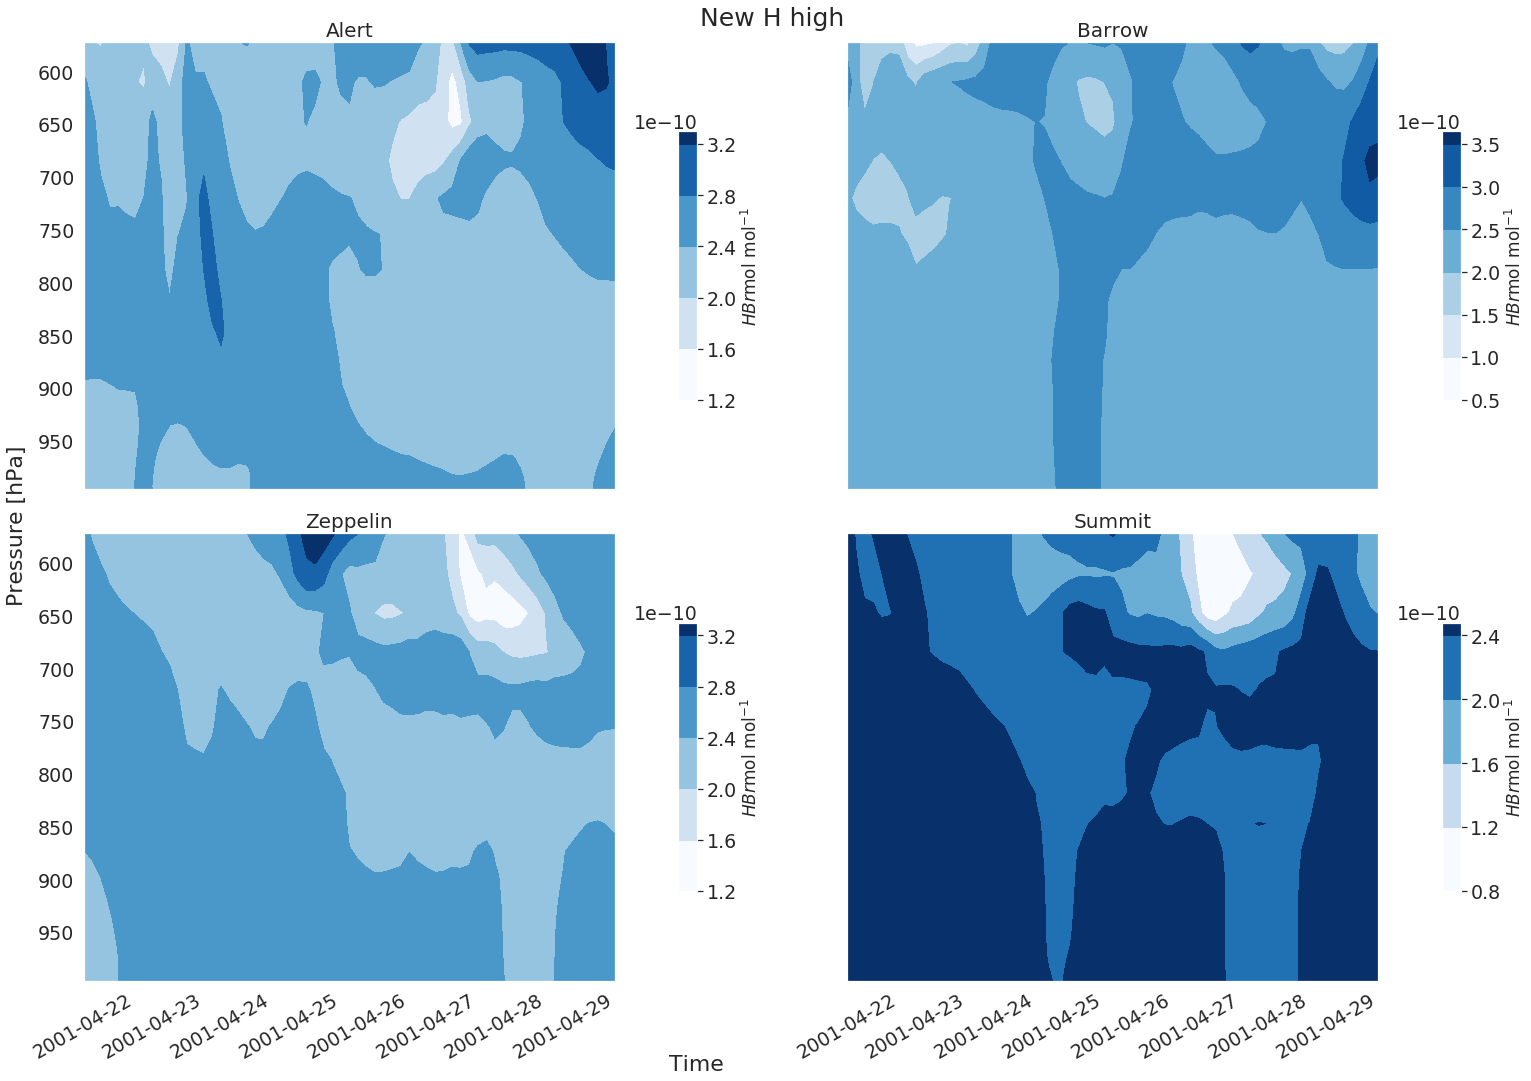
\includegraphics[width=\linewidth]{Chapter6_Results/images/vertHBr_HFOUR_step3.png}
    \caption{Mixing ratio ($mol mol^{-1}$) of \chem{HBr} in the model layers up to $\sim 600 hPa$ at the four different stations Alert (top left), Barrow (top right), Zeppelin (lower left) and Summit (lower right) in April, 2001. The result is from the test including hard-coded photodissociation rates as well as a new (high) Henry-coefficient at HFOUR resolution}
    \label{fig:vertHBr_HFOUR_step3}
\end{figure}
\begin{figure}[h]
    \centering
    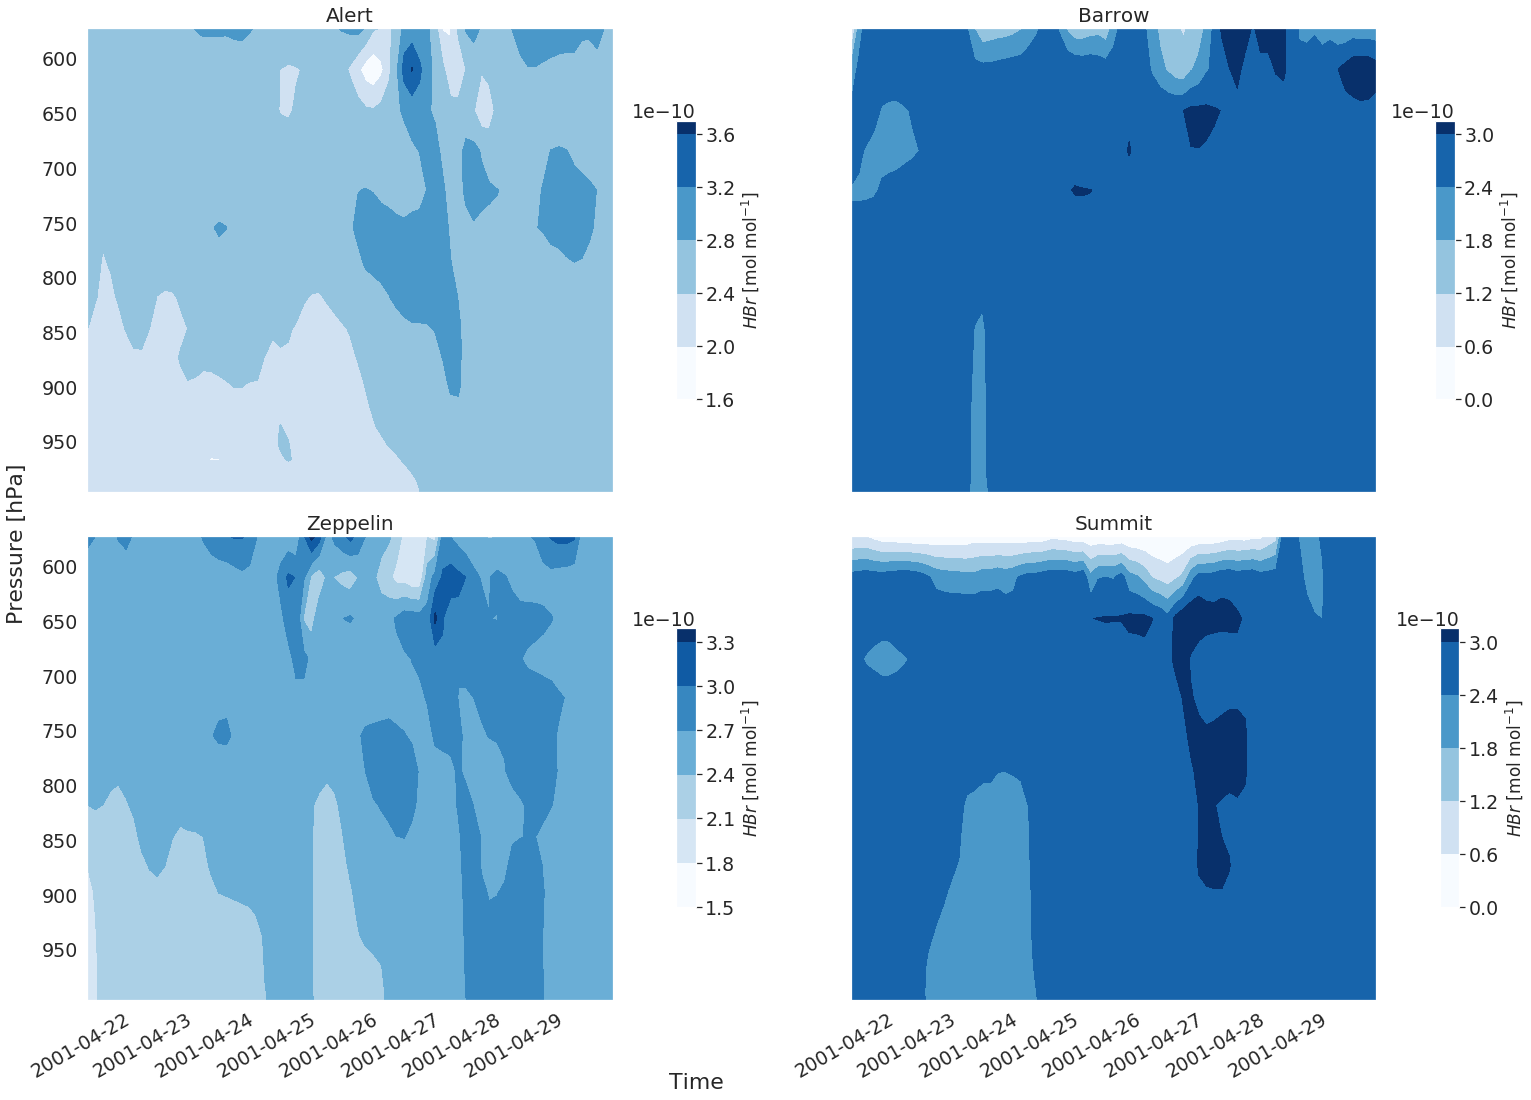
\includegraphics[width=\linewidth]{Chapter6_Results/images/Vert_StationComp_2001/vertHBr_HTWO_step3.png}
    \caption{Mixing ratio ($mol mol^{-1}$) of \chem{HBr} in the model layers up to $\sim 600 hPa$ at the four different stations Alert (top left), Barrow (top right), Zeppelin (lower left) and Summit (lower right) in April, 2001. The result is from Branch \ref{def:BE_PD_noCl} including hard-coded photodissociation rates as well as a new (high) Henry-coefficient at HTWO resolution}
    \label{fig:vertHBr_HTWO_step3}
\end{figure}

%\begin{figure}[h]
    \centering
    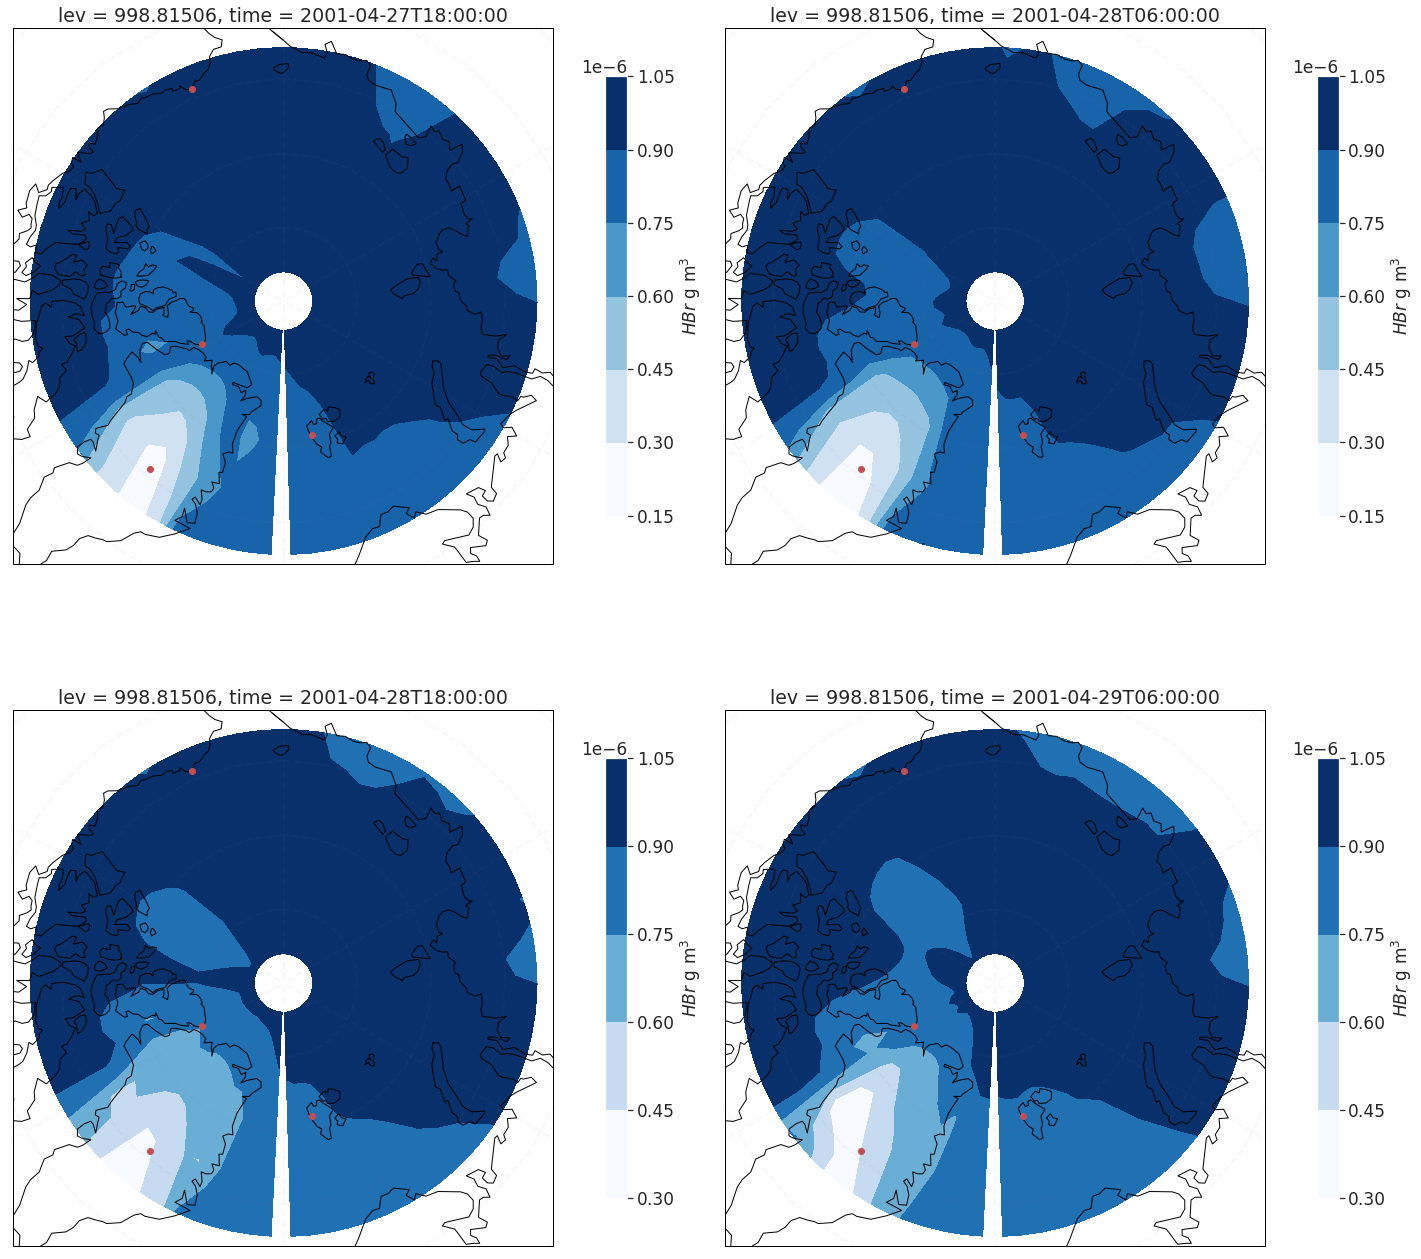
\includegraphics[width=\linewidth]{Chapter6_Results/images/polarHBr_HFOUR_step3.png}
    \caption{Concentration ($g m^{-3}$) of \chem{HBr} in the first model layer the Arctic at 18:00 and 06:00 (UTC) of the 27th, 28th and 29th of April, 2001. The result is from the test including hard-coded photodissociation rates as well as a new (high) Henry-coefficient at HFOUR resolution. The red dots are the positions of the stations with observations in 2001 (see the map in Figure \ref{fig:stns} for reference)}
    \label{fig:polarHBr_HFOUR_step3}
\end{figure}
\begin{figure}[h]
    \centering
    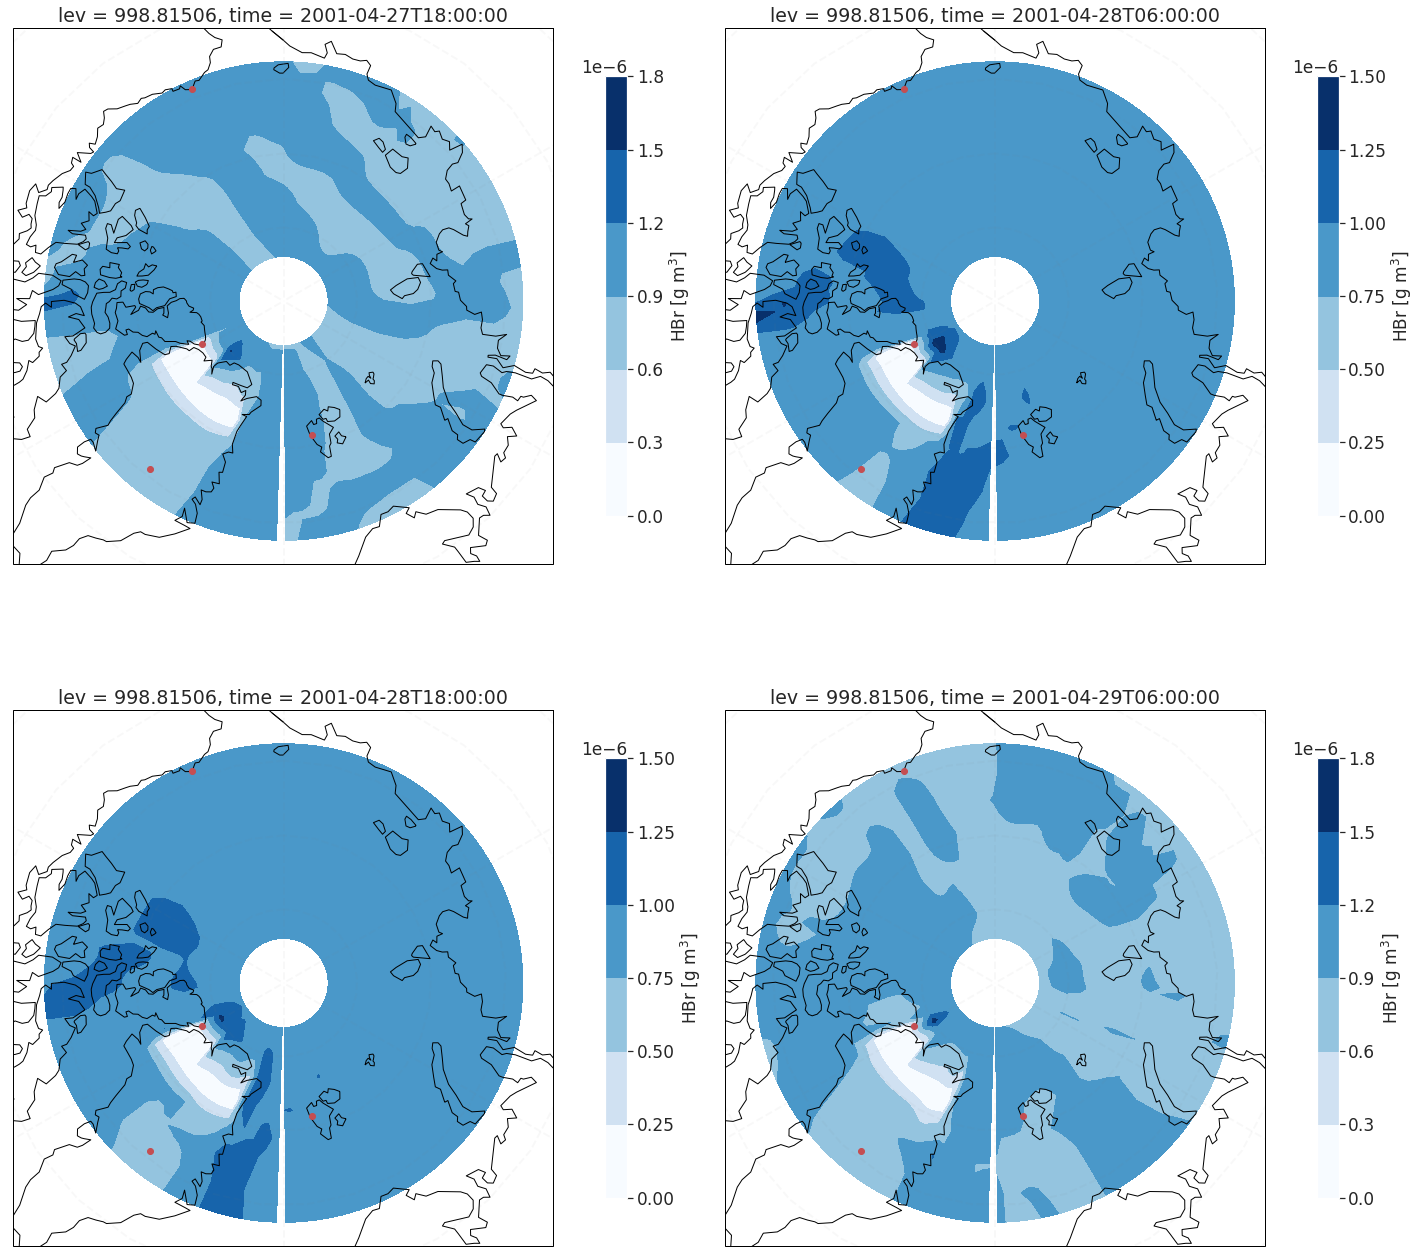
\includegraphics[width=\linewidth]{Chapter6_Results/images/Polar_StationComp_2001/HBr/polarHBr_HTWO_step3.png}
    \caption{Concentration ($g m^{-3}$) of \chem{HBr} in the first model layer the Arctic at 18:00 and 06:00 (UTC) of the 27th, 28th and 29th of April, 2001. The result is from Branch \ref{def:BE_PD_noCl} including hard-coded photodissociation rates as well as a new (high) Henry-coefficient at HTWO resolution. The red dots are the positions of the stations with observations in 2001 (see the map in Figure \ref{fig:stns} for reference)}
    \label{fig:polarHBr_HTWO_step3}
\end{figure}

\begin{figure}[h]
    \centering
    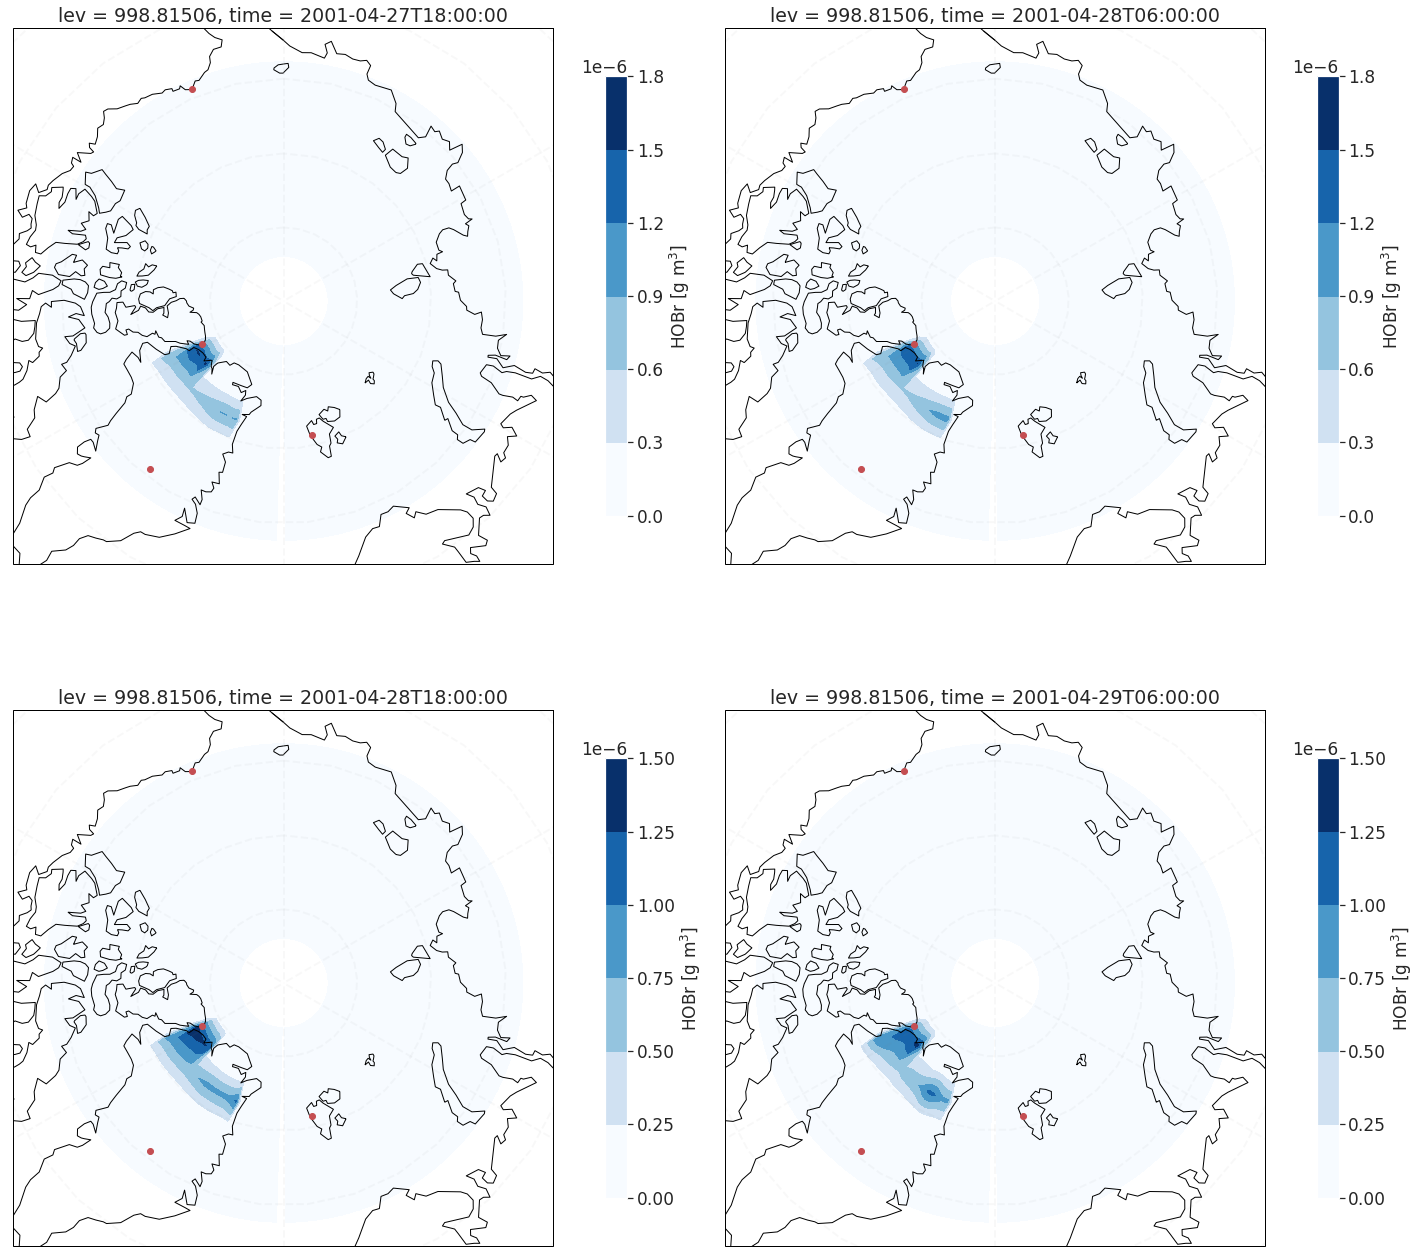
\includegraphics[width=\linewidth]{Chapter6_Results/images/Polar_StationComp_2001/HOBr/polarHOBr_HTWO_step3.png}
    \caption{Concentration ($g m^{-3}$) of \chem{HOBr} in the first model layer the Arctic at 18:00 and 06:00 (UTC) of the 27th, 28th and 29th of April, 2001. The result is from  Branch \ref{def:BE_PD_noCl} including hard-coded photodissociation rates as well as a new (high) Henry-coefficient at HTWO resolution. The red dots are the positions of the stations with observations in 2001 (see the map in Figure \ref{fig:stns} for reference)}
    \label{fig:polarHOBr_HTWO_step3}
\end{figure}
%\begin{figure}[h]
    \centering
    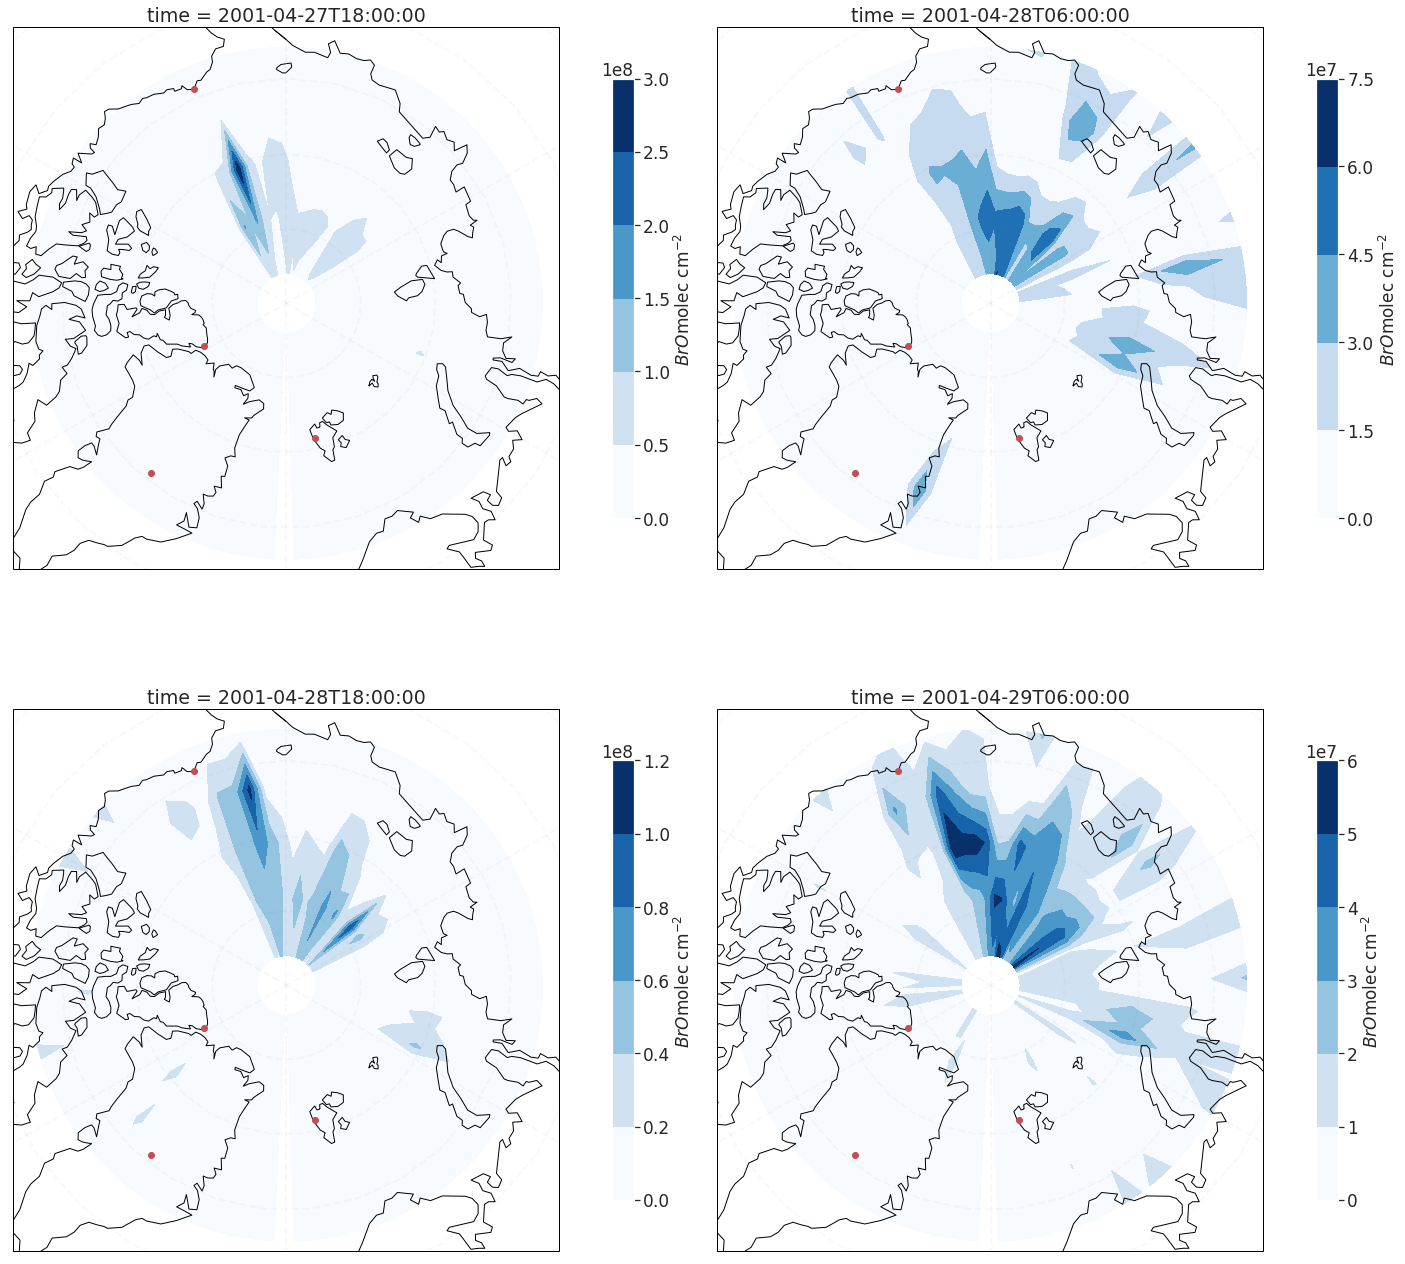
\includegraphics[width=\linewidth]{Chapter6_Results/images/polarBrO_HFOUR_step3.png}
    \caption{Vertical column density ($molecules cm^{-2}$) of \chem{BrO} in the lowermost $\sim 250 m$ at 18:00 and 06:00 (UTC) of the 27th, 28th and 29th of April, 2001. The result is from the test including hard-coded photodissociation rates as well as a new (high) Henry-coefficient at HFOUR resolution. The red dots are the positions of the stations with observations in 2001 (see the map in Figure \ref{fig:stns} for reference)}
    \label{fig:polarBrO_HFOUR_step3}
\end{figure}
\begin{figure}[h]
    \centering
    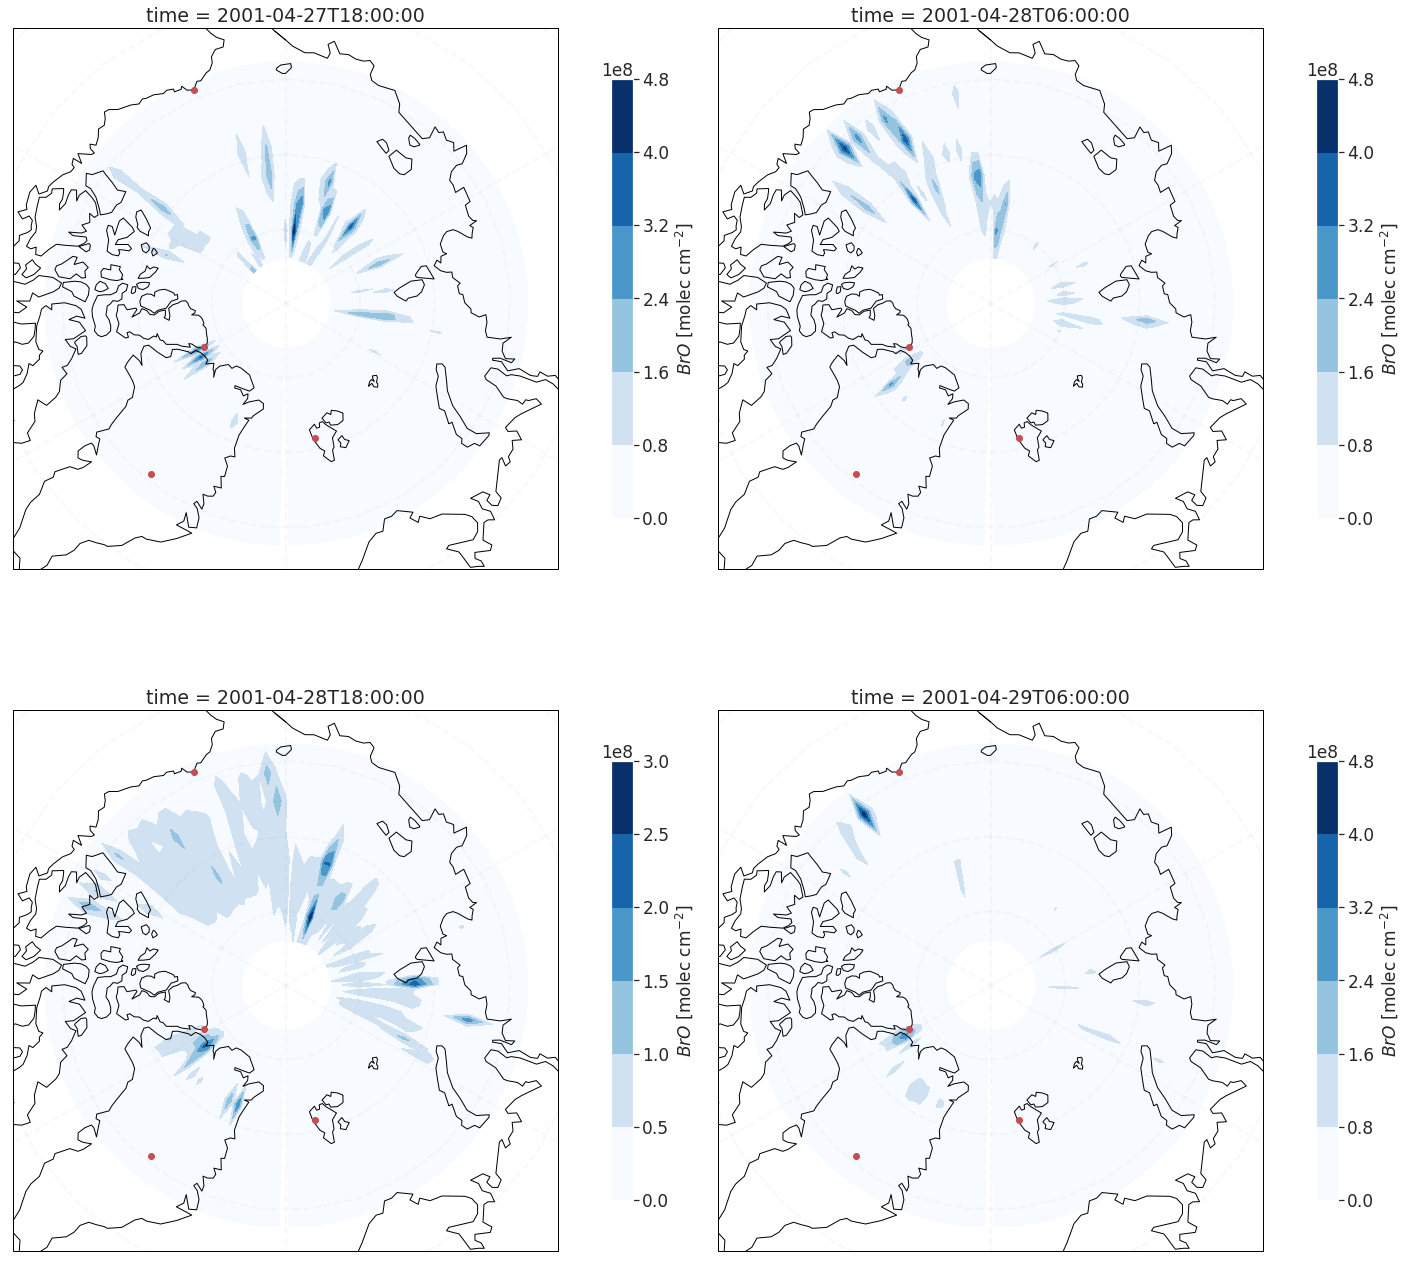
\includegraphics[width=\linewidth]{Chapter6_Results/images/Polar_StationComp_2001/BrO/polarBrO_HTWO_step3.png}
    \caption{Vertical column density ($molecules cm^{-2}$) of \chem{BrO} in the lowermost $\sim 250 m$ at 18:00 and 06:00 (UTC) of the 27th, 28th and 29th of April, 2001. The result is from  Branch \ref{def:BE_PD_noCl} including hard-coded photodissociation rates as well as a new (high) Henry-coefficient at HFOUR resolution. The red dots are the positions of the stations with observations in 2001 (see the map in Figure \ref{fig:stns} for reference)}
    \label{fig:polarBrO_HTWO_step3}
\end{figure}

\clearpage
\section{Analysis of the Final Version of the Halogen Branch}\label{app:final_version}

\begin{figure}[h]
    \centering
    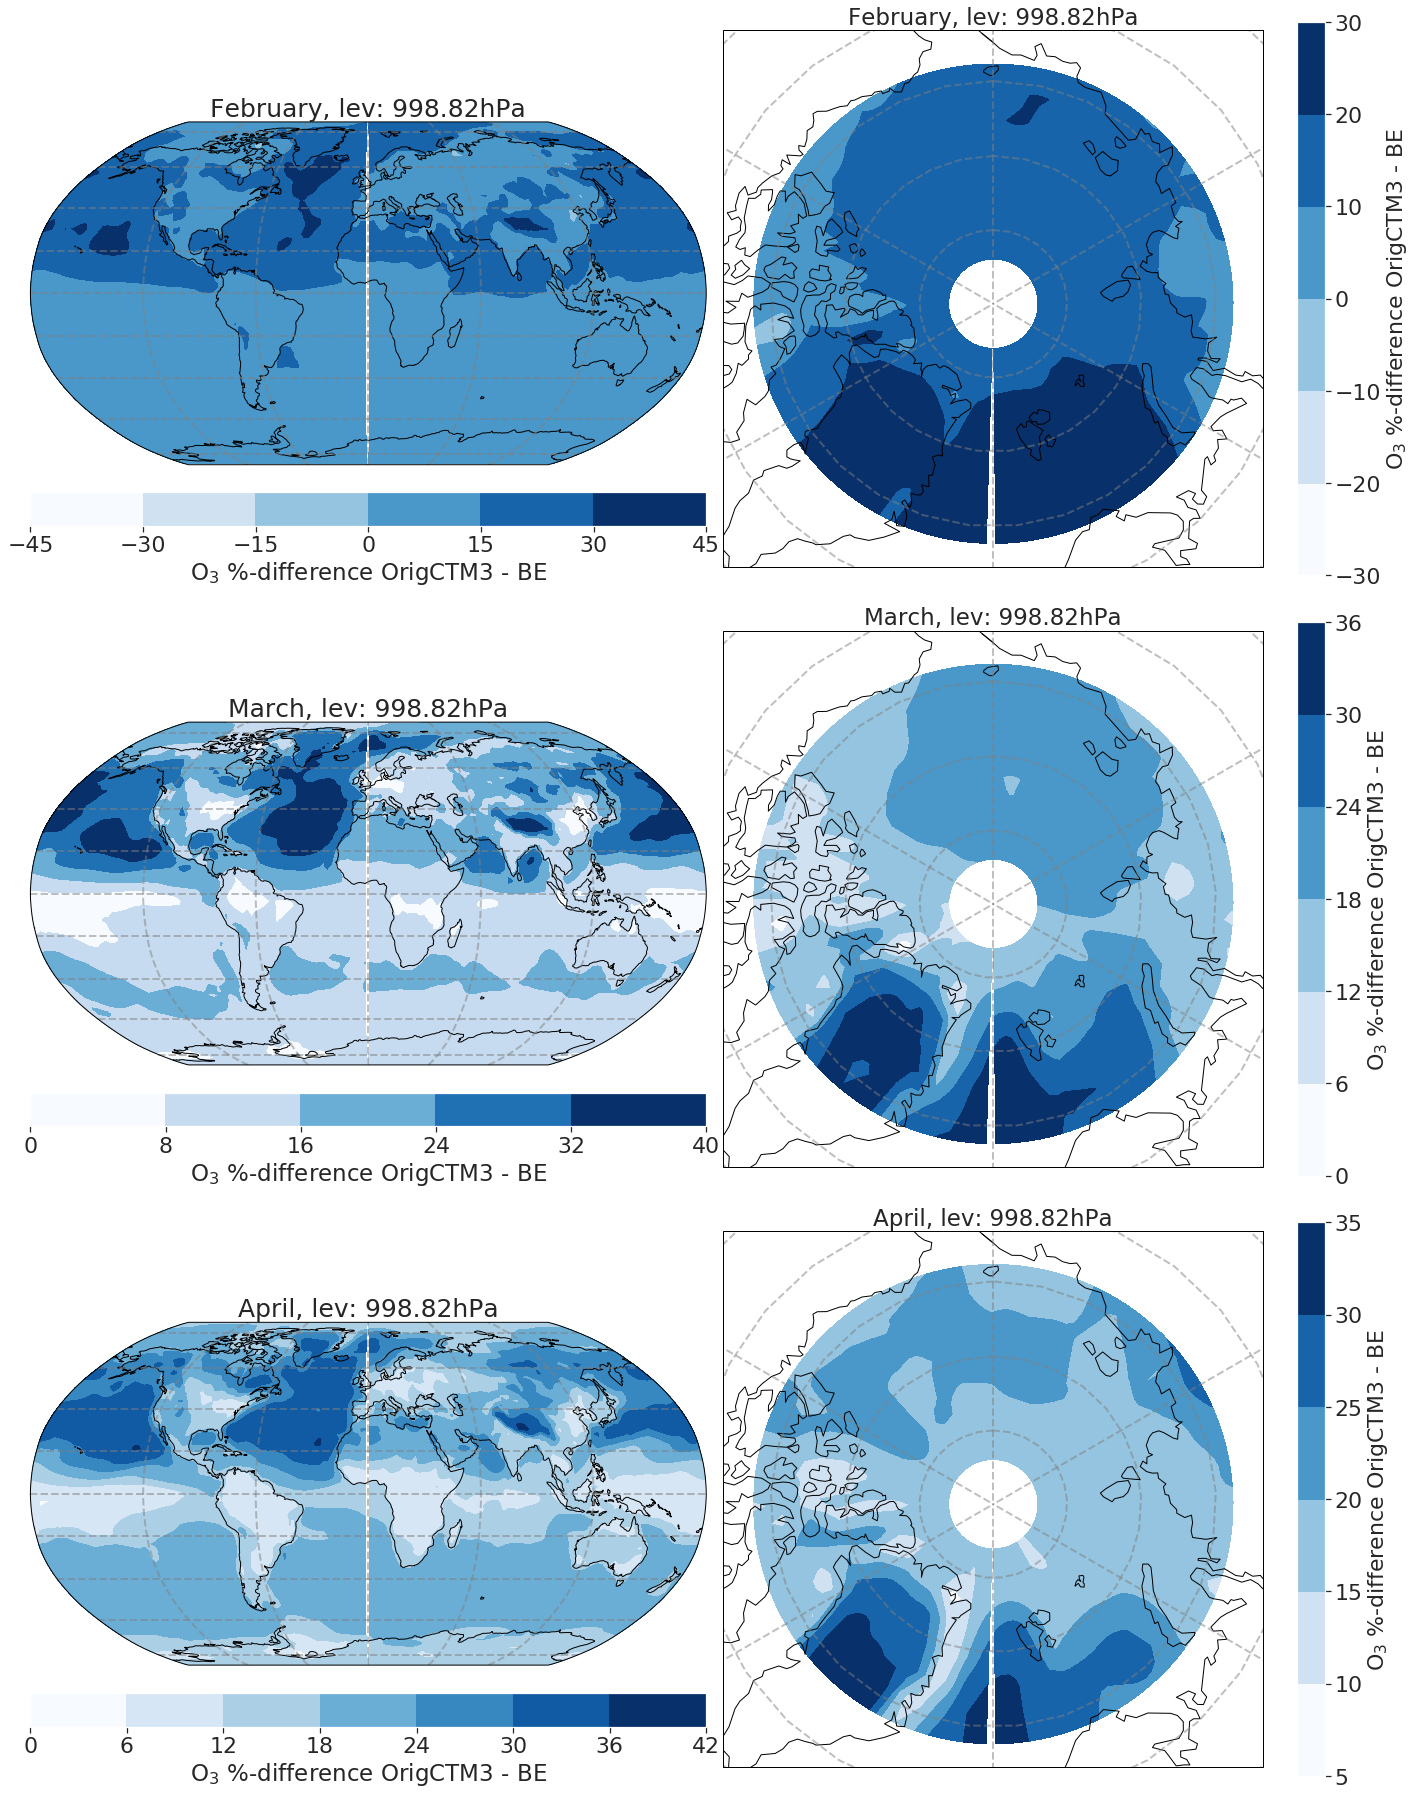
\includegraphics[width = \linewidth]{Chapter6_Results/images/Orig_BE_comp/BE_origPD_vmr_lev0_FebApr_2001.png}
    \caption{Difference in ozone monthly mean volume mixing ratio (in ppb) in the first model layer between the original CTM3 and the BE-branch globally (left columns) and in the Arctic (right columns) in the months February (top figures), March (middle figures) and April (bottom figures) in 2001. \textbf{Note:} the colorbar axis are not equal}
    \label{fig:BE_origPD_vmr_FebApr}
\end{figure}


%%% SKAL TIL APPENDIX

\begin{figure}[h]
    \centering
    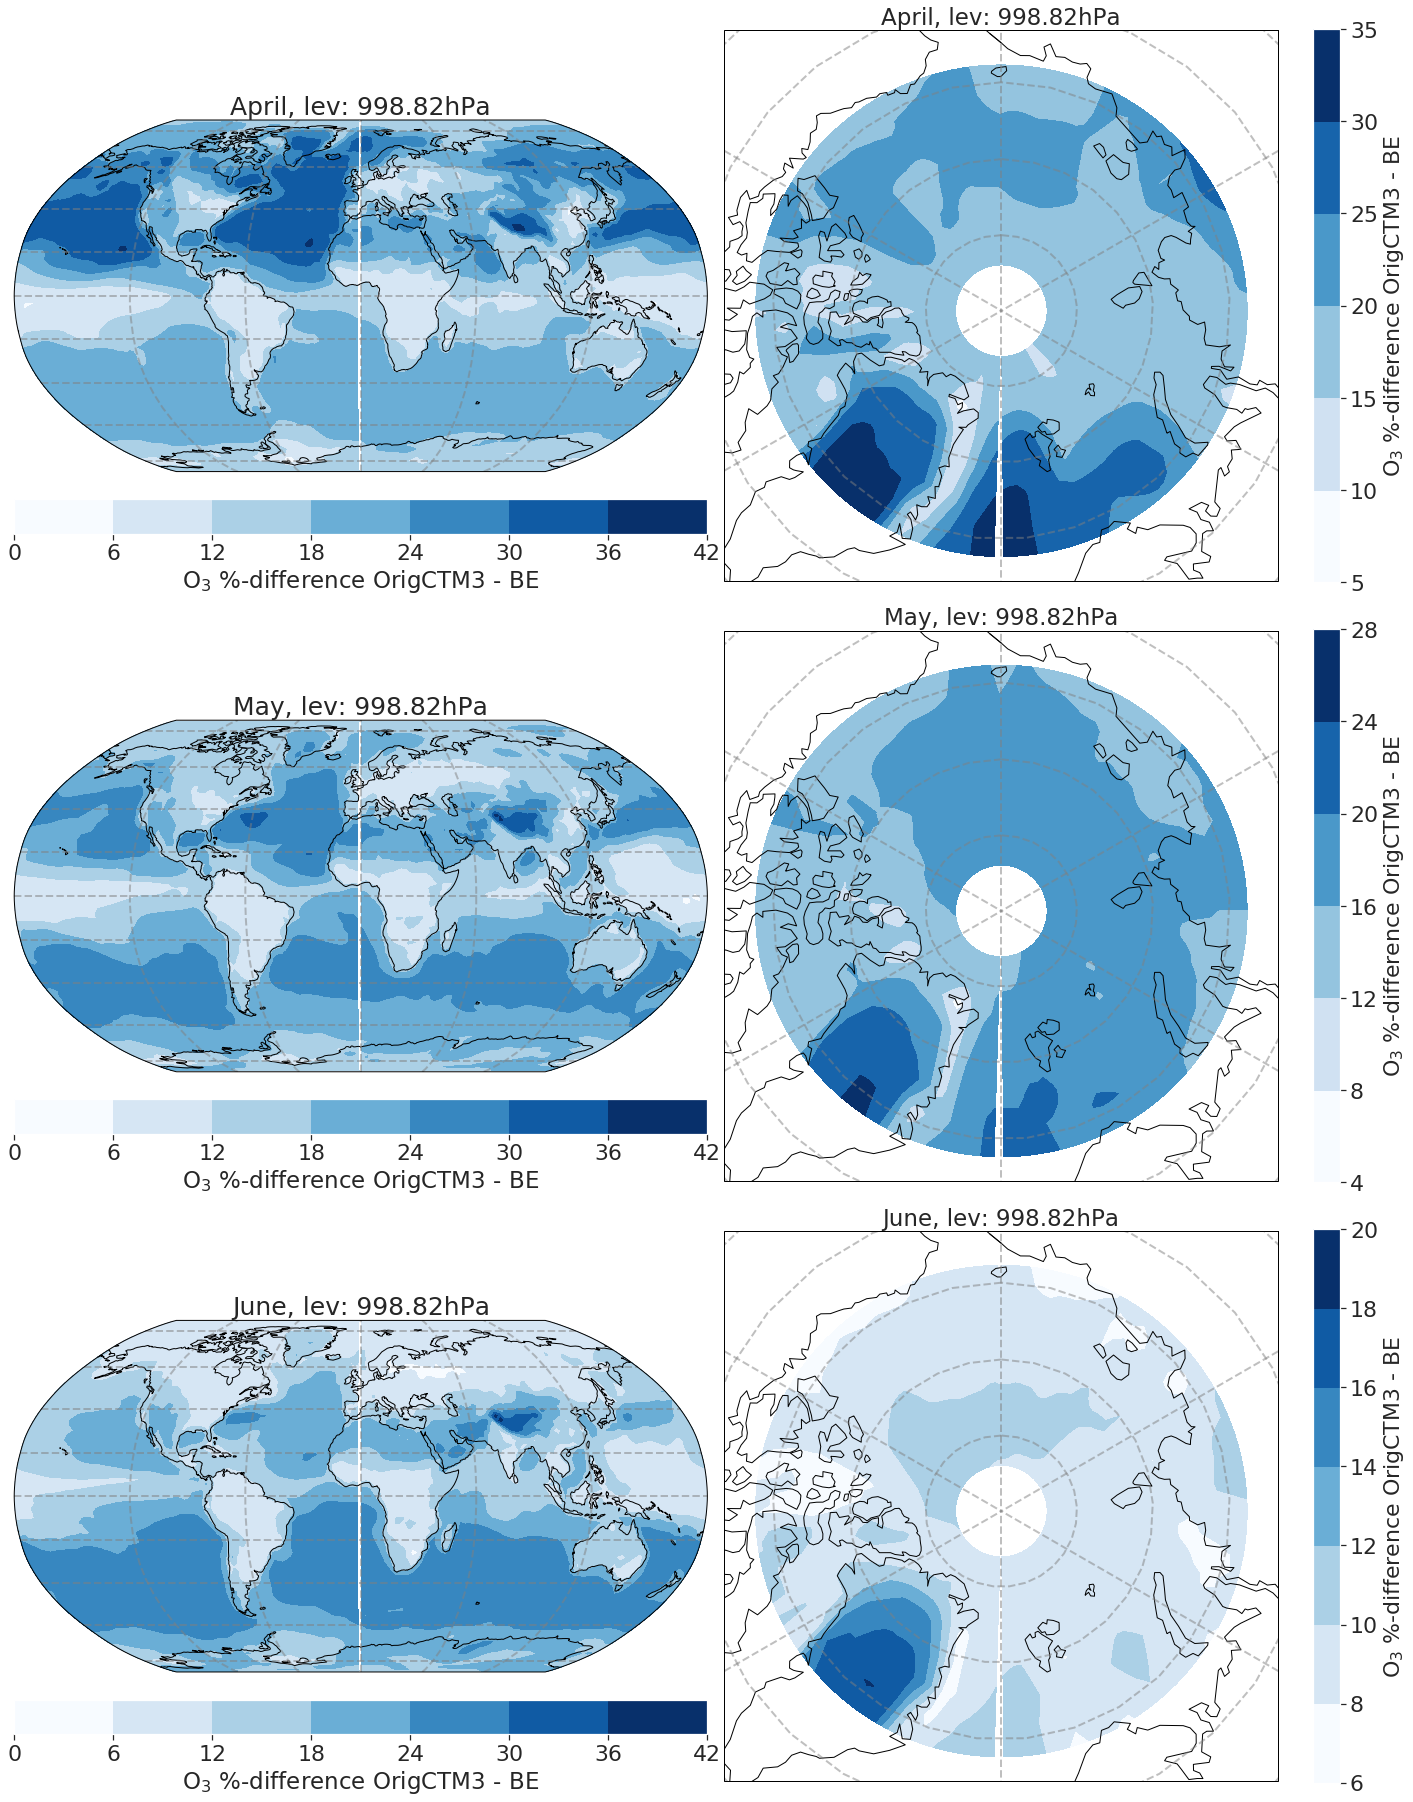
\includegraphics[width = \linewidth]{Chapter6_Results/images/Orig_BE_comp/BE_origPD_vmr_lev0_AprJune_2001.png}
    \caption{Difference in ozone monthly mean volume mixing ratio (in ppb) in the first model layer between the original CTM3 and the BE-branch globally (left columns) and in the Arctic (right columns) in the months April (top figures), May (middle figures) and June (bottom figures) in 2001 \textbf{Note:} the colorbar axis are not equal}
    \label{fig:BE_origPD_vmr_AprJun}
\end{figure}


%%% SKAL TIL APPENDIX

\begin{figure}[h]
    \centering
    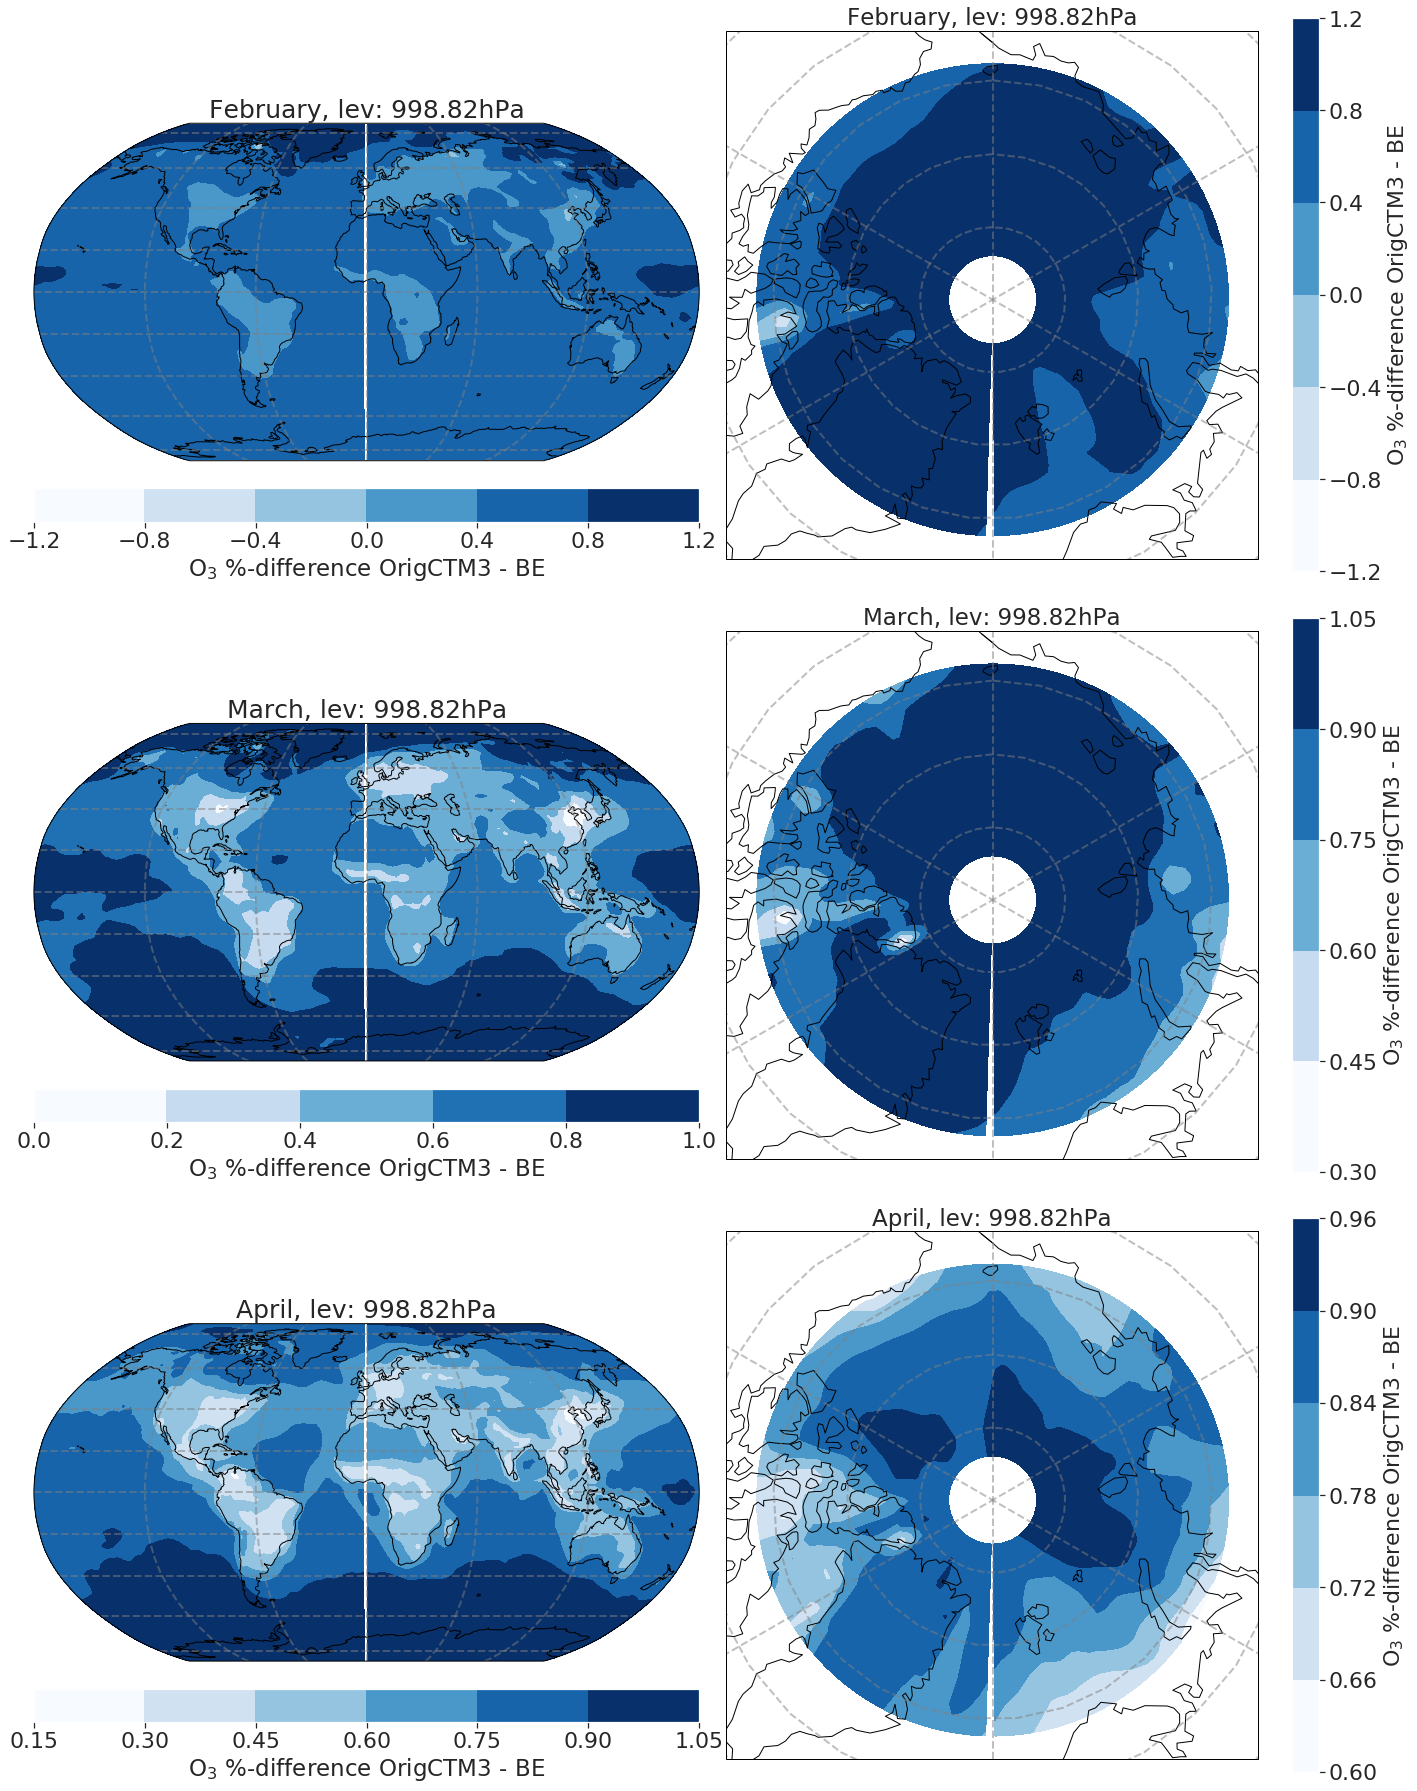
\includegraphics[width = \linewidth]{Chapter6_Results/images/Orig_BE_comp/BE_origPD_percent_lev0_FebApr_2001.png}
    \caption{Percentage difference in ozone monthly mean in the first model layer between the original CTM3 and the BE-branch globally (left columns) and in the Arctic (right columns) in the months February (top figures), March (middle figures) and April (bottom figures) in 2001 \textbf{Note:} the colorbar axis are not equal}
    \label{fig:BE_origPD_percent_FebApr}
\end{figure}


%%% SKAL TIL APPENDIX

\begin{figure}[h]
    \centering
    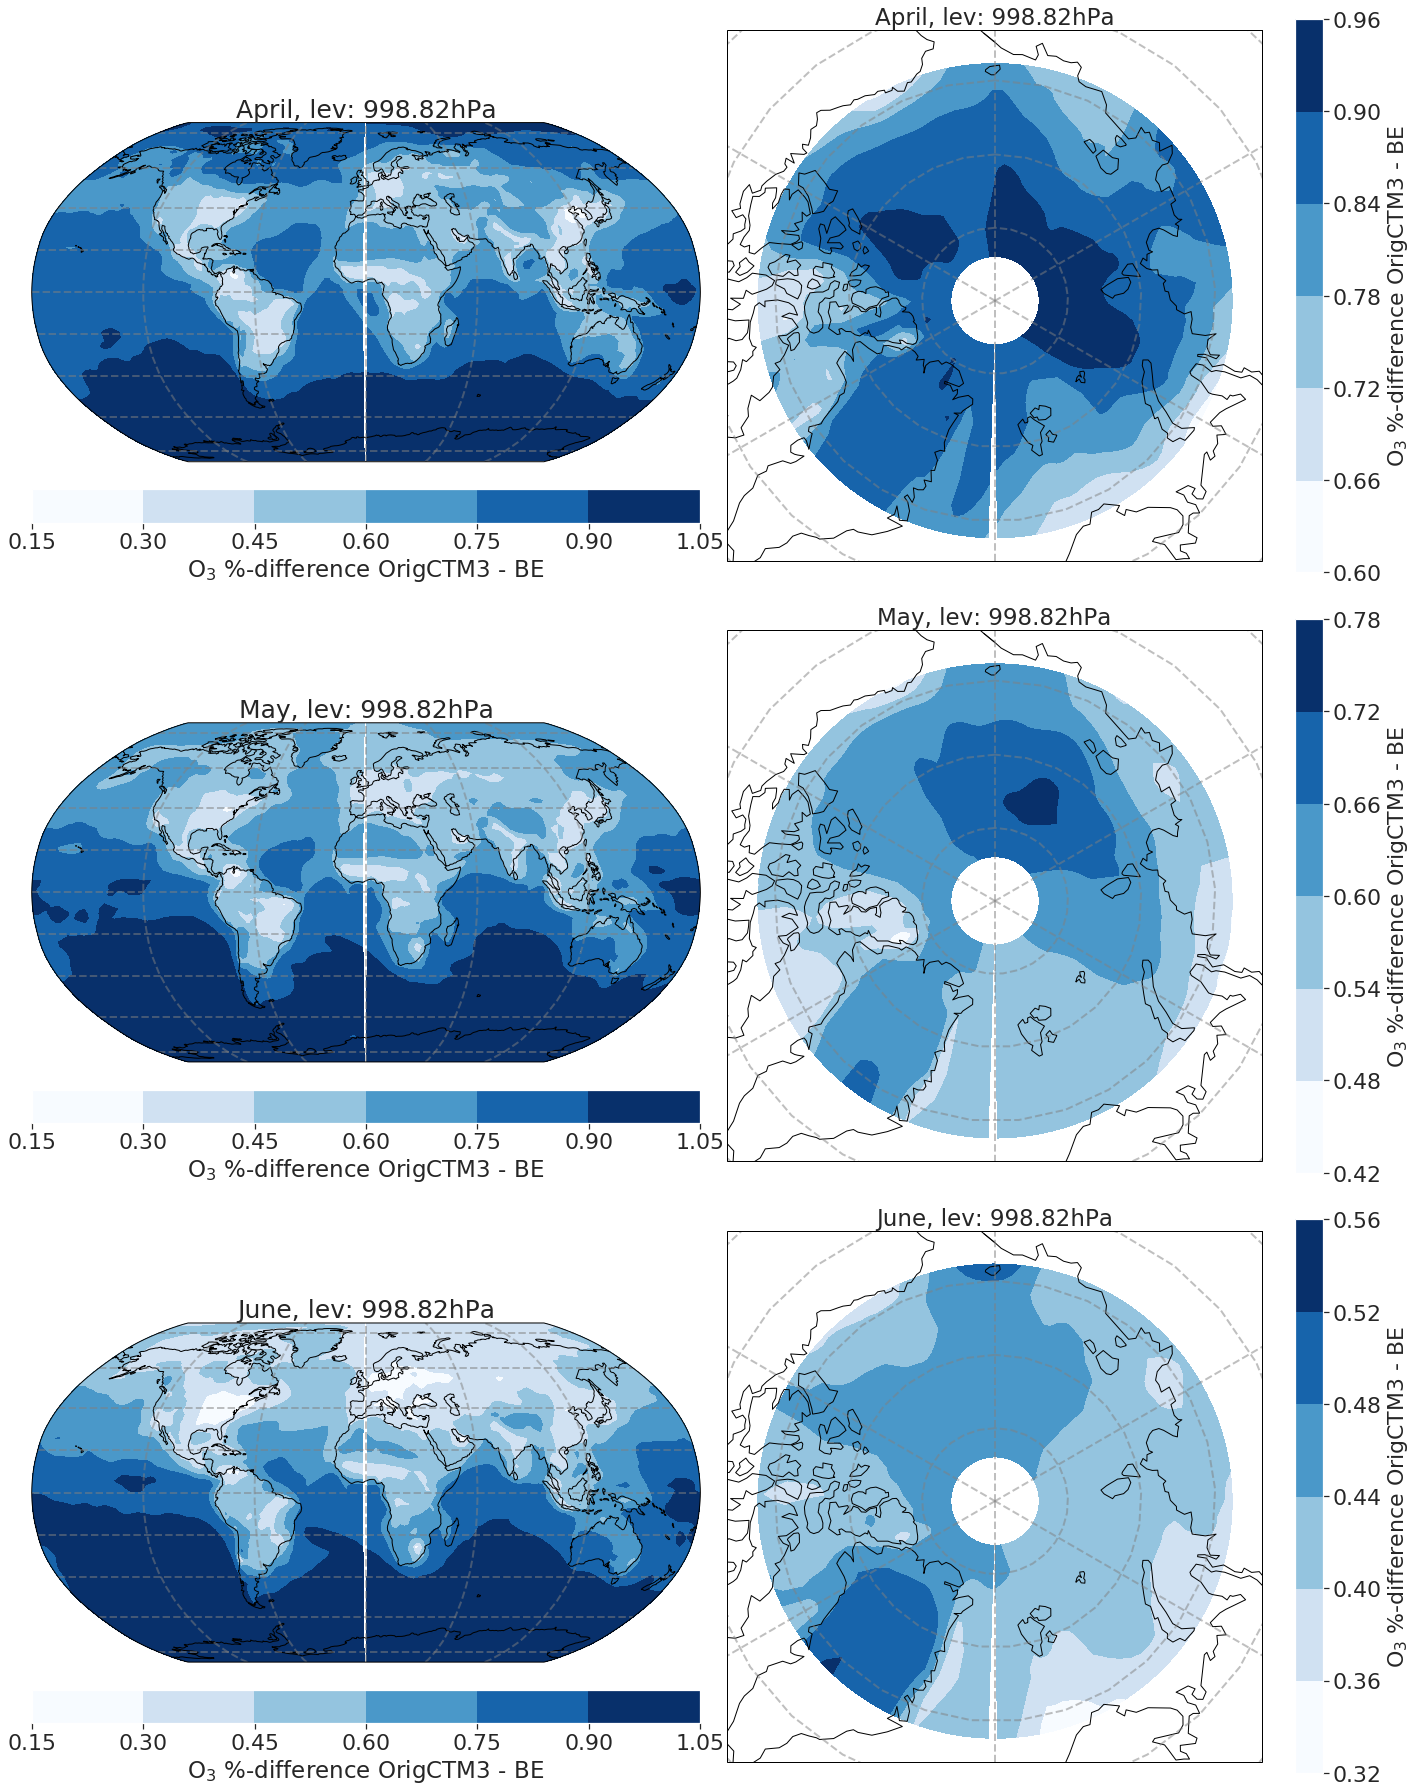
\includegraphics[width = \linewidth]{Chapter6_Results/images/Orig_BE_comp/BE_origPD_percent_lev0_AprJune_2001.png}
    \caption{Percentage difference in ozone monthly mean in the first model layer between the original CTM3 and the BE-branch globally (left columns) and in the Arctic (right columns) in the months April (top figures), May (middle figures) and June (bottom figures) in 2001 \textbf{Note:} the colorbar axis are not equal}
    \label{fig:BE_origPD_percent_AprJun}
\end{figure}

%%% SKAL TIL APPENDIX

\clearpage
\section{Radiative Forcing}\label{app:RF}

%%% SKAL TIL APPENDIX

\begin{figure}[ht]
    \centering
    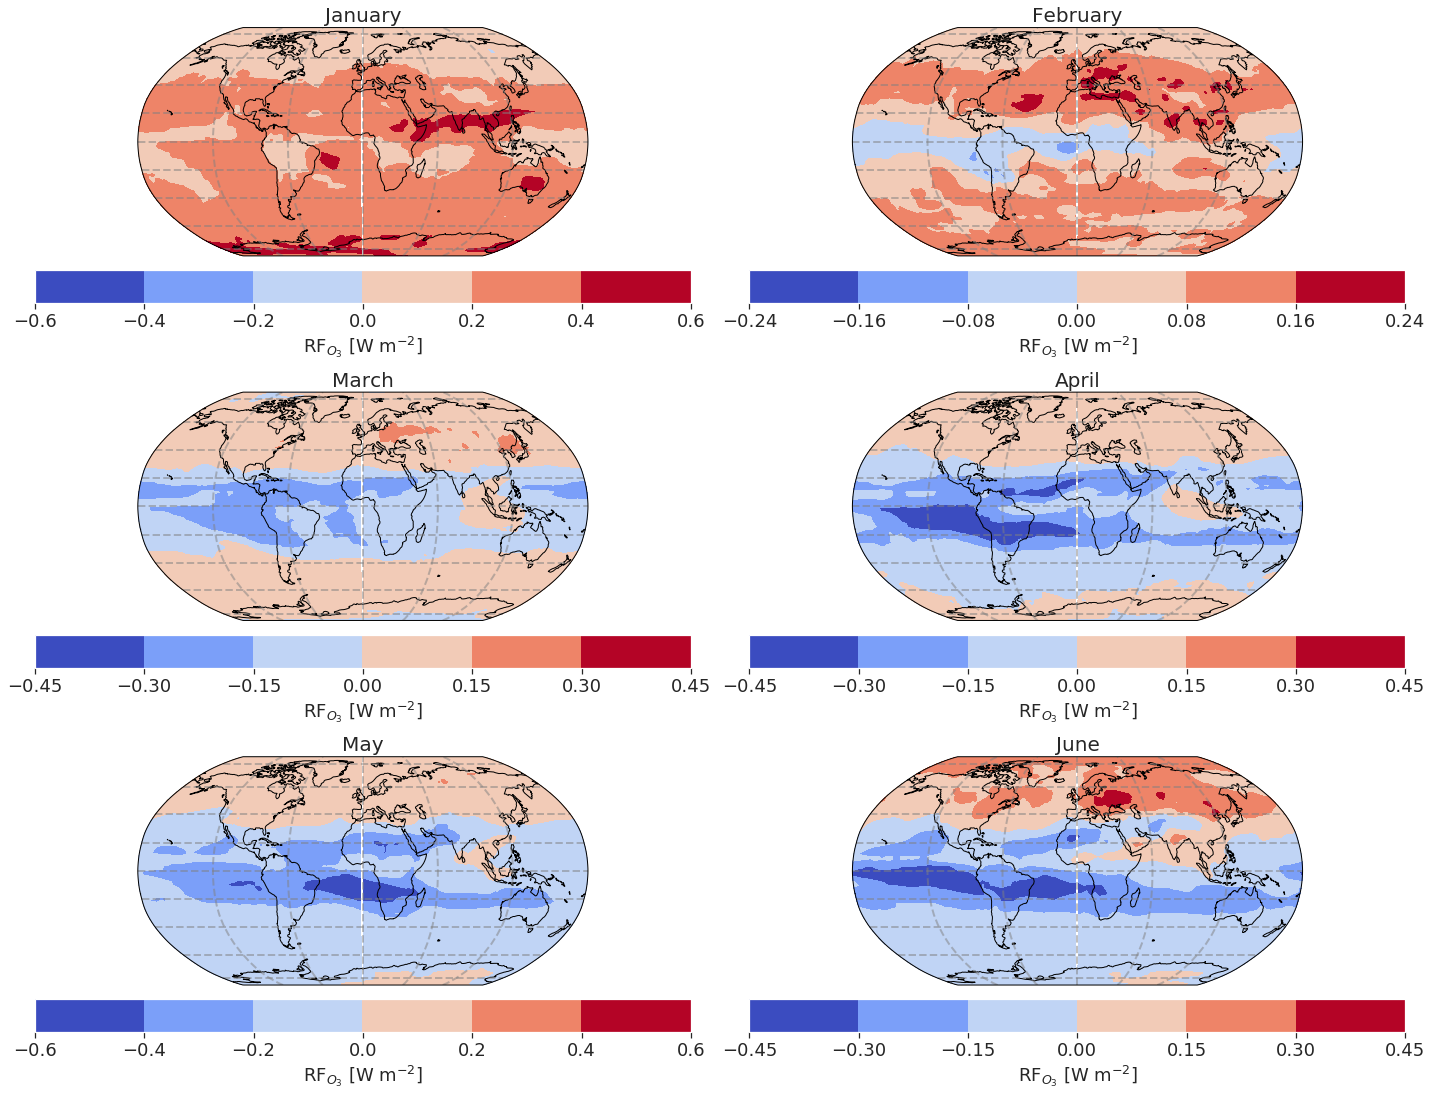
\includegraphics[width = \linewidth]{Chapter6_Results/images/RF/BE_RF_global_2001.png}
    \caption{Global RF-field (in Wm$^{-2}$) for the total tropospheric column up to the tropopause, produced using the BE-branch in 2001}
    \label{fig:BE_RF_global_2001}
\end{figure}

\begin{figure}[ht]
    \centering
    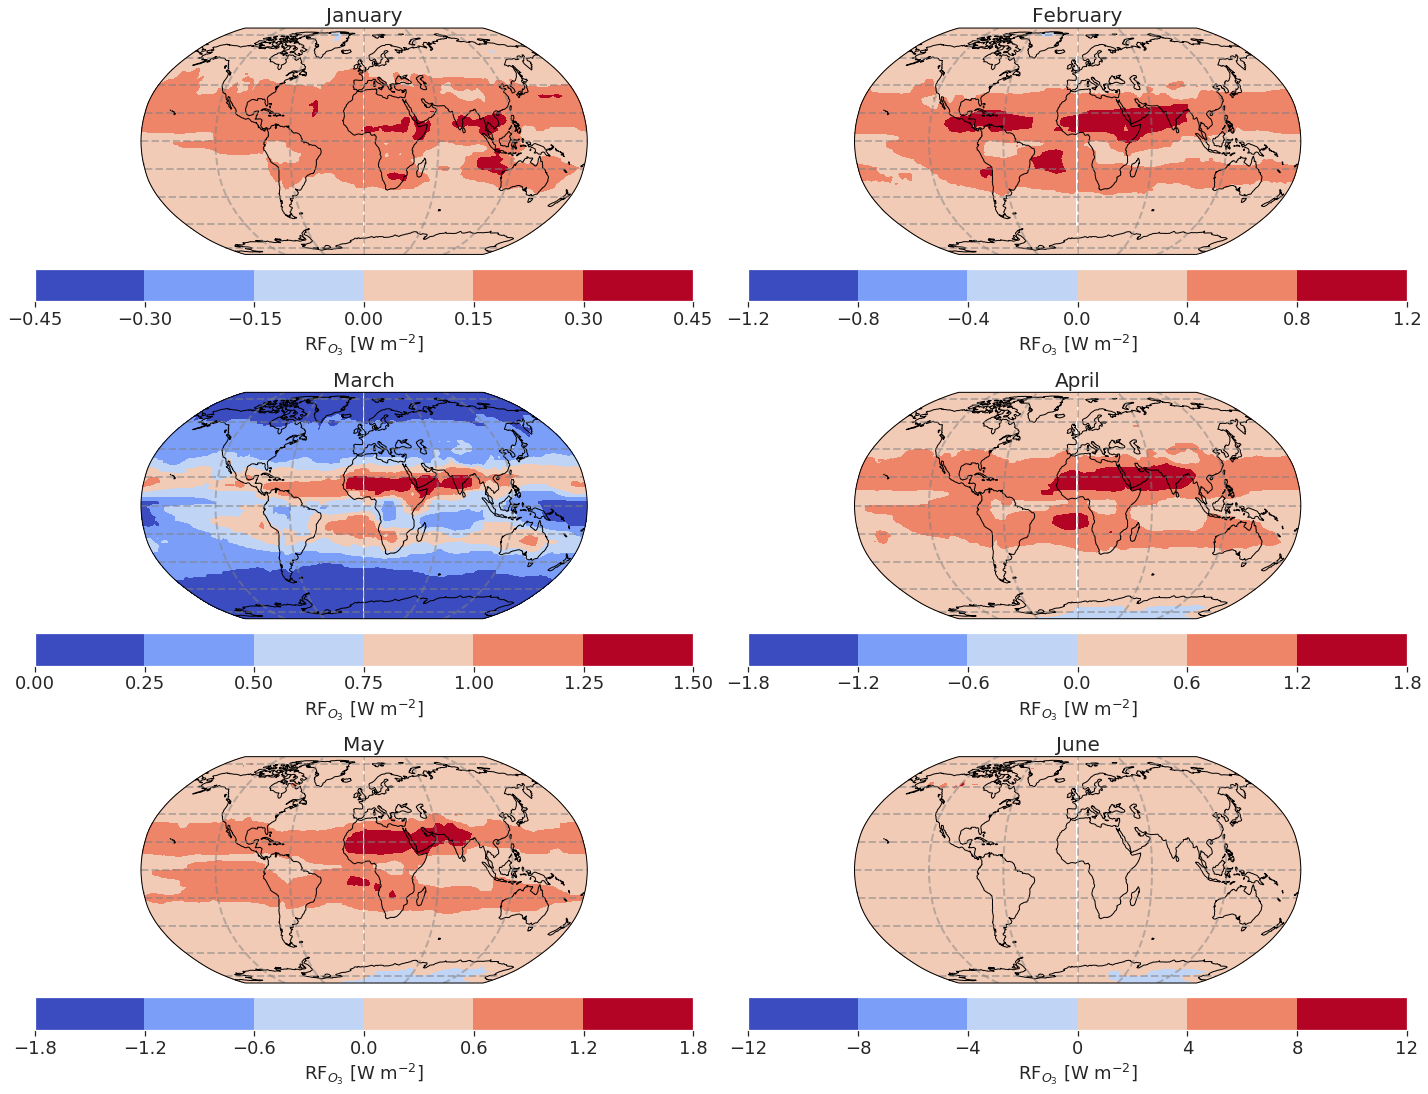
\includegraphics[width = \linewidth]{Chapter6_Results/images/RF/RF_USE/Appendix/BE_RF_global_2013.png}
    \caption{Global RF-field (in Wm$^{-2}$) for the total tropospheric column up to the tropopause, produced using the BE-branch in 2013}
    \label{fig:BE_RF_global_2013}
\end{figure}

\begin{figure}[ht]
    \centering
    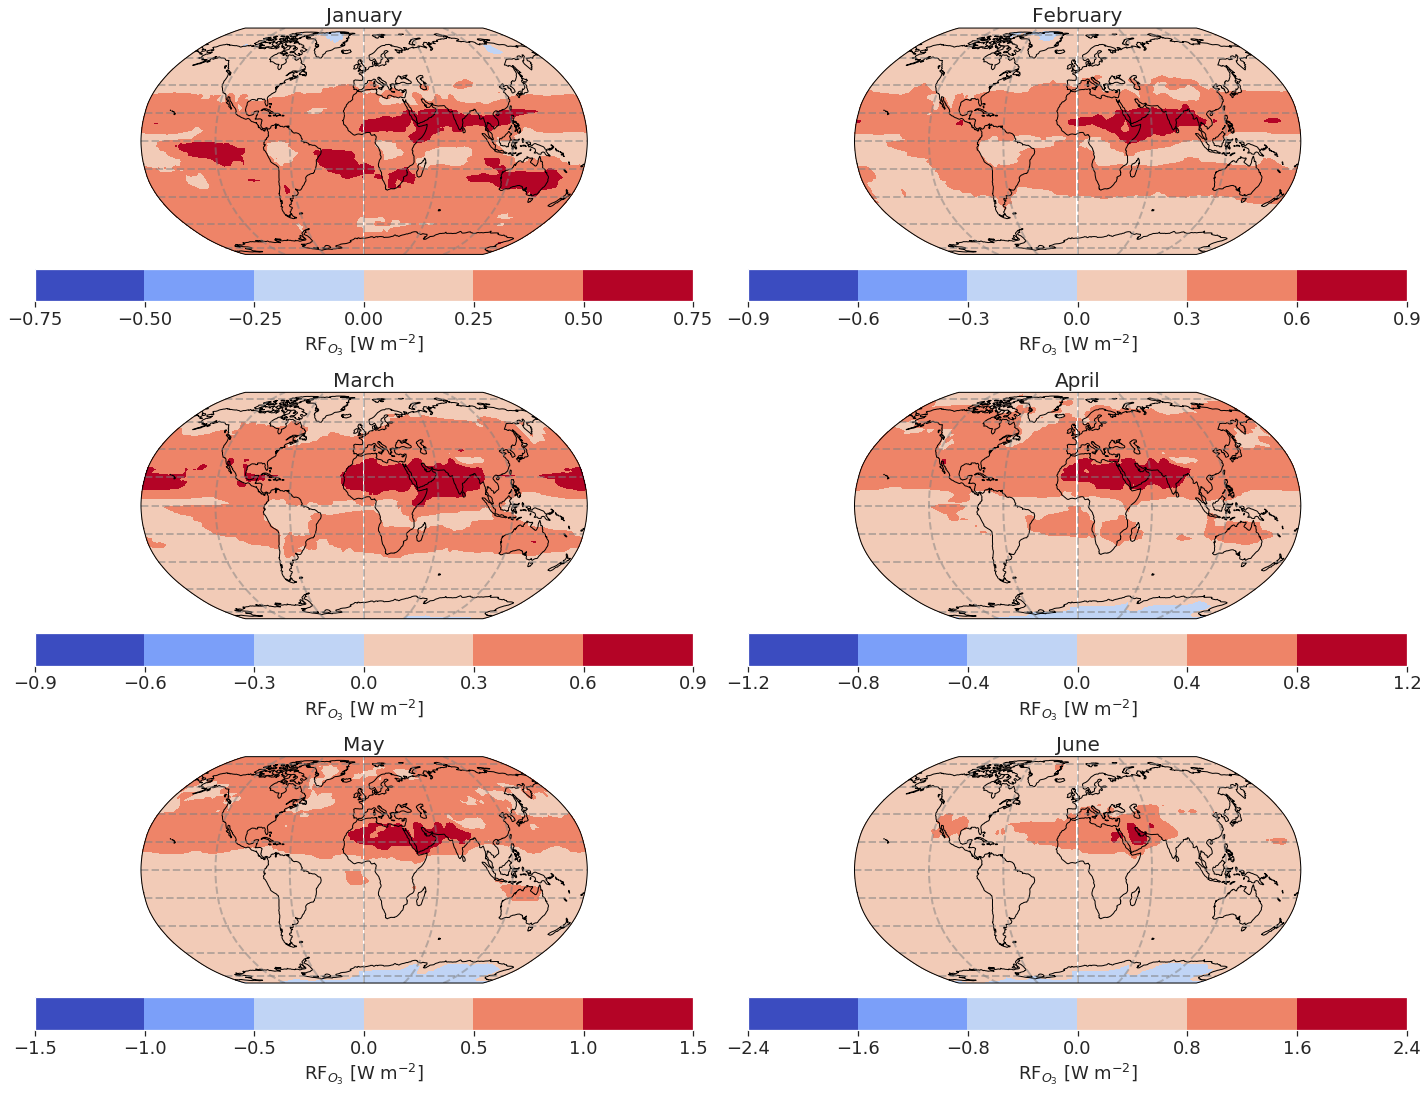
\includegraphics[width = \linewidth]{Chapter6_Results/images/RF/RF_USE/Appendix/Orig_RF_global_2001.png}
    \caption{Global RF-field (in Wm$^{-2}$) for the total tropospheric column up to the tropopause, produced using the Original CTM3 in 2001}
    \label{fig:orig_RF_global_2001}
\end{figure}
\begin{figure}[ht]
    \centering
    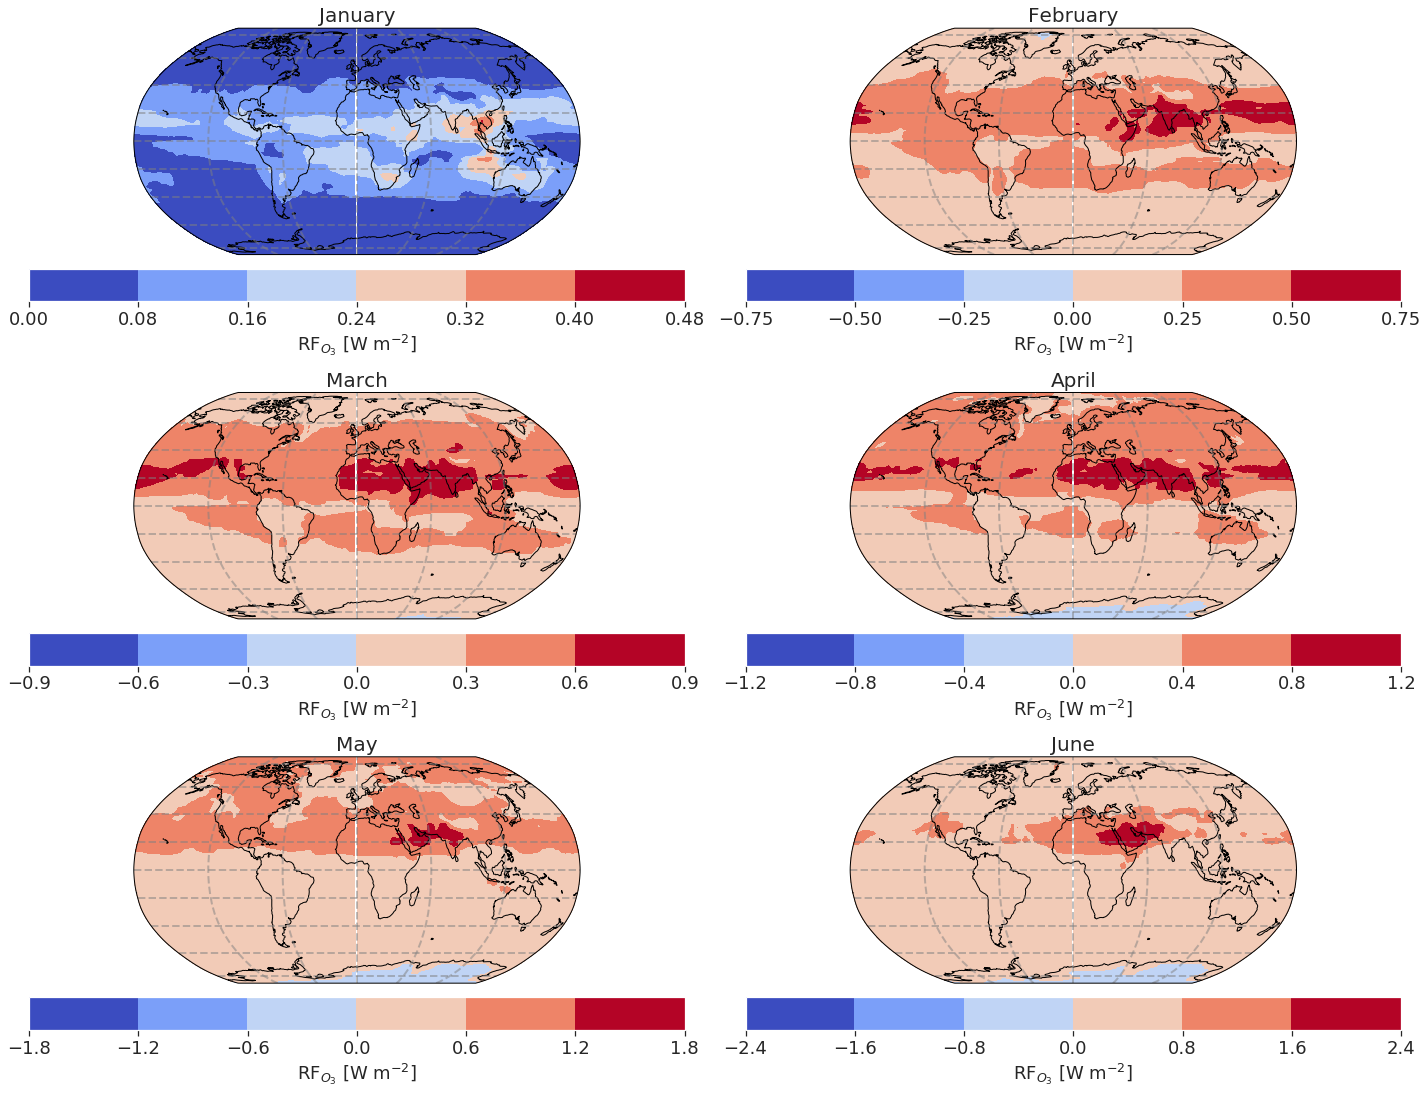
\includegraphics[width = \linewidth]{Chapter6_Results/images/RF/RF_USE/Appendix/Orig_RF_global_2013.png}
    \caption{Global RF-field (in Wm$^{-2}$) for the total tropospheric column up to the tropopause, produced using the Original CTM3 in 2013. \textbf{Note:} the colorbar axis are not equal}
    \label{fig:orig_RF_global_2013}
\end{figure}

\cleardoublepage

\printbibliography
\cleardoublepage

\end{document}
